 % The main file for CAMP reports
 % Don't put any content in here. 
 % Don't even include content files by using \input or \inlcude. 
 % Put your content to TEXT.TEX or include it there using \input.
 % Uses:
 %		SETTINGS.TEX	contains the settings for this document
 %		COMMANDS.TEX	contains commands which can be used while writing
 %		INFO.TEX			contains the author, title and so on for the cover
 %		COVER.TEX			formats\documentclass[10pt]{?} the front cover of the document
 %		ABSTRACT.TEX	contains the abstract to be included (if needed)
 %		TEXT.TEX			contains the actual content of the document
 %		BIB.BIB				containt the BibTeX entries for the document
 
 
%% Draft document mode
%% Final document
\documentclass[11pt,a4paper,bibtotoc,idxtotoc,headsepline,footsepline,footexclude,BCOR12mm,DIV13]{scrbook}


%\documentclass[11pt,a4paper,bibtotoc,idxtotoc,headsepline,footsepline,footexclude,BCOR20mm,DIV10]{scrbook}

% KOMA-Optionen:
%  bibtotoc: include bibliography in table of contents
%  idxtotoc: include index in table of contents
%  headsepline: use horizontalline under heading
%  BCOR: binding correcion (Bindungskorrektur) (e.g.: BCOR5mm)
%  DIV: Number of sheet sections (used for layout) (e.g.: DIV12) 


% include title and author information for the cover
% Set here the title, authors and other stuff to be used for the cover
% This file is used by MAIN.TEX

% set title, authors and stuff for the cover
\def\doctype{Master's Thesis in Informatics}
\def\title{Materialized views with Apache Spark}
\def\titleGer{Materialisierte views mit Apache Spark}
\def\author{Saroj Gautam}
\def\date{August 15th, 2016}

% text to appear in the footer
\def\footertext{}

% include settings
% Included by MAIN.TEX
% Defines the settings for the CAMP report document

\renewcommand{\sectfont}{\normalfont \bfseries}        % Schriftart der Kopfzeile

% manipulate footer
\usepackage{scrpage2}
\pagestyle{scrheadings}
\ifoot[\footertext]{\footertext} % \footertext set in INFO.TEX
%\setkomafont{pagehead}{\normalfont\rmfamily}
\setkomafont{pagenumber}{\normalfont\rmfamily}

%% allow sophisticated control structures
\usepackage{ifthen}

% use Palatino as default font
\usepackage{palatino}

% enable special PostScript fonts
\usepackage{pifont}

% make thumbnails
\usepackage{thumbpdf}

%to use the subfigures
%\usepackage{subfigure}
\usepackage{caption}
\usepackage{subcaption}


\usepackage{colortbl}


%% show program code\ldots
%\usepackage{verbatim}
%\usepackage{program}

\usepackage{listings}


%% enable TUM symbols on title page
\usepackage{styles/tumlogo}


\usepackage{multirow}

%% use colors
\usepackage{color}

%% make fancy math
\usepackage{amsmath}
\usepackage{amsfonts}
\usepackage{amssymb}
\usepackage{textcomp}
\usepackage{yhmath} % f�r die adots 
%% mark text as preliminary
%\usepackage[draft,german,scrtime]{prelim2e}

%% create an index
\usepackage{makeidx}

% for the program environment
\usepackage{float}

%% load german babel package for german abstract
%\usepackage[german,american]{babel}
\usepackage[german,english]{babel}
\selectlanguage{english}

% use german characters as well
\usepackage[latin1]{inputenc}       % allow Latin1 characters

% use initals dropped caps - doesn't work with PDF
%\usepackage{dropping}

% Load the package
\usepackage{glossaries}

\usepackage{styles/shortoverview}
%----------------------------------------------------
%      Graphics and Hyperlinks
%----------------------------------------------------

%% check for pdfTeX
\ifx\pdftexversion\undefined
 %% use PostScript graphics
 \usepackage[dvips]{graphicx}
 \DeclareGraphicsExtensions{.eps,.epsi}
 \graphicspath{{figures/}{figures/review}} 
 %% allow rotations
 \usepackage{rotating}
 %% mark pages as draft copies
 %\usepackage[english,all,light]{draftcopy}
 %% use hypertex version of hyperref
 \usepackage[hypertex,hyperindex=false,colorlinks=false]{hyperref}
\else %% reduce output size \pdfcompresslevel=9
 %% declare pdfinfo
 %\pdfinfo { 
 %  /Title (my title) 
 %  /Creator (pdfLaTeX) 
 %  /Author (my name) 
 %  /Subject (my subject	) 
 %  /Keywords (my keywords)
 %}
 %% use pdf or jpg graphics
 \usepackage[pdftex]{graphicx}
 \DeclareGraphicsExtensions{.jpg,.JPG,.png,.pdf,.eps}
 \graphicspath{{figures/}} 
 
 %% Load float package, for enabling floating extensions
 \usepackage{float}
 
 %% allow rotations
 \usepackage{rotating}
 %% use pdftex version of hyperref
 \usepackage[pdftex,colorlinks=true,linkcolor=black,citecolor=black,%
 anchorcolor=black,urlcolor=black,bookmarks=true,%
 bookmarksopen=true,bookmarksopenlevel=0,plainpages=false%
 bookmarksnumbered=true,hyperindex=false,pdfstartview=%
 ]{hyperref}
%
%\usepackage[pdftex,colorlinks=false,linkcolor=red,citecolor=red,%
% anchorcolor=red,urlcolor=red,bookmarks=true,%
% bookmarksopen=true,bookmarksopenlevel=0,plainpages=false%
% bookmarksnumbered=true,hyperindex=false,pdfstartview=%
% ]{hyperref}
\fi




%% Fancy chapters
%\usepackage[Lenny]{fncychap}
%\usepackage[Glenn]{fncychap}
%\usepackage[Bjarne]{fncychap}

%\usepackage[avantgarde]{quotchap}

% set the bibliography style
%\bibliographystyle{styles/bauermaNum}
%\bibliographystyle{alpha}
\bibliographystyle{plain}

% include commands
% Commands to be used within the TUM report document
% Included by MAIN.TEX
% Please include your own cool commands here. 
% Be only sure to comment it sufficiently so others can use it.

%-------------------------------------------------------------
%                      Own Commands
%-------------------------------------------------------------


%-------------------------------------------------------------
% math stuff -------------------------------------------------

% nice R, N, C
\newcommand{\nat}{\mathbb{N}}
\newcommand{\real}{\mathbb{R}}
\newcommand{\compl}{\mathbb{C}}



% norm
\newcommand{\norm}[1]{\left\| #1 \right\|}

% un demi
\newcommand{\half}{\frac{1}{2}}

% parantheses
\newcommand{\parenth}[1]{ \left( #1 \right) }
\newcommand{\bracket}[1]{ \left[ #1 \right] }
\newcommand{\accolade}[1]{ \left\{ #1 \right\} }
%\newcommand{\angle}[1]{ \left\langle  #1 \right\rangle }

% partial derivative: %#1 function, #2 which variable
% simple / single line version
\newcommand{\pardevS}[2]{ \delta_{#1} f(#2) }
% fraction version
\newcommand{\pardevF}[2]{ \frac{\partial #1}{\partial #2} }

% render vectors: 3 and 4 dimensional
\newcommand{\veciii}[3]{\left[ \begin{array}[h]{c} #1 \\ #2 \\ #3	\end{array} \right]}
\newcommand{\veciv}[4]{\left[ \begin{array}[h]{c} #1 \\ #2 \\ #3 \\ #4	\end{array} \right]}

% render matrices: 3  dimensional (arguments in row first order)
\newcommand{\matiii}[9]{\left[ \begin{array}[h]{ccc} #1 & #2 & #3 \\ #4 & #5 & #6 \\ #7 & #8 & #9	\end{array} \right]}
%DOESN'T WORK,DON'T KNOW WHY \newcommand{\mativ}[16]{\left[ \begin{array}[h]{cccc} #1 & #2 & #3 & #4 \\ #5 & #6 & #7 & #8 \\ #9 & #10 & #11 & #12 \\ #13 & #14 & #15 & #16 \end{array} \right]}


%-------------------------------------------------------------
%-------------------------------------------------------------


%-------------------------------------------------------------
% some abreviations ------------------------------------------
\newcommand{\Reg}{$^{\textregistered}$}
\newcommand{\reg}{$^{\textregistered}$ }
\newcommand{\Tm}{\texttrademark}
\newcommand{\tm}{\texttrademark~}
\newcommand {\bsl} {$\backslash$}

%-------------------------------------------------------------
%-------------------------------------------------------------


%-------------------------------------------------------------
% formating --------------------------------------------------

% Theorem & Co environments and counters
\newtheorem{theorem}{Theorem}[chapter]
\newtheorem{lemma}[theorem]{Lemma}
\newtheorem{corollary}[theorem]{Corollary}
\newtheorem{remark}[theorem]{Remark}
\newtheorem{definition}[theorem]{Definition}
\newtheorem{equat}[theorem]{Equation}
\newtheorem{example}[theorem]{Example}
\newtheorem{algorithm}[theorem]{Algorithm}

% inserting figures
\newcommand{\insertfigure}[4]{ % Filename, Caption, Label, Width percent of textwidth
	\begin{figure}[htbp]
		\begin{center}
			\includegraphics[width=#4\textwidth]{#1}
		\end{center}
		\vspace{-0.4cm}
		\caption{#2}
		\label{#3}
	\end{figure}
}




% referecing figures

\newcommand{\refFigure}[1]{ %label
	figure \ref{#1}
}
\newcommand{\refChapter}[1]{ %label
	chapter \ref{#1}
}

\newcommand{\refSection}[1]{ %label
	section \ref{#1}
}

\newcommand{\refParagraph}[1]{ %label
	paragraph \ref{#1}
}

\newcommand{\refEquation}[1]{ %label
	equation \ref{#1}
}

\newcommand{\refTable}[1]{ %label
	table \ref{#1}
}




\newcommand{\rigidTransform}[2]
{
	${}^{#2}\!\mathbf{H}_{#1}$
}

%code, in typewriter
\newcommand{\code}[1]
 {\texttt{#1}}

% comment that appears on the border - very practical !!!
\newcommand{\comment}[1]{\marginpar{\raggedright \noindent \footnotesize {\sl #1} }}

% page clearing
\newcommand{\clearemptydoublepage}{%
  \ifthenelse{\boolean{@twoside}}{\newpage{\pagestyle{empty}\cleardoublepage}}%
  {\clearpage}}


%-------------------------------------------------------------
%-------------------------------------------------------------


\newcommand{\etAl}{\emph{et al.}\mbox{ }}


%\makeindex
	%% inter line spacing
%\linespread{1.0}

\makeglossary

\begin{document}

	\frontmatter
	
	
	% The front cover for the TUM report document.
% Included by MAIN.TEX


%--------------------------------------------------
% The Front Cover
%--------------------------------------------------

% The front cover for the TUM document.
% Included by MAIN.TEX


%--------------------------------------------------
% The Front Cover
%--------------------------------------------------

% correct BCOR - undo at the end !!!
\def\bcorcor{0.15cm}
\addtolength{\hoffset}{\bcorcor}

\thispagestyle{empty}

 \vspace{4cm}
\begin{center}
	       \oTUM{4cm}
	   
	   \vspace{5mm}     
	   \huge FAKULT{\"A}T F{\"U}R INFORMATIK\\ 
	   \vspace{0.5cm}
	 \large DER TECHNISCHEN UNIVERSIT{\"A}T M{\"U}NCHEN\\
    \vspace{1mm}
        
	\end{center}
		

\vspace{15mm}
\begin{center}

   {\Large \doctype}

  \vspace{20mm}
  
  {\huge\bf \title}\\%[3ex]
  
  
  \vspace{15mm}
  
  
  {\LARGE  \author}
  
  \vspace{10mm}
  
  \begin{figure}[h!]
  \centering
   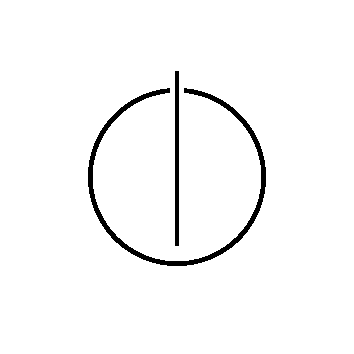
\includegraphics[width=4cm]{styles/informat.png}
  \end{figure}
  
  \end{center}
%	\clearemptydoublepage
	
	%% The titlepage for the CAMP report document.
% Included by MAIN.TEX


%--------------------------------------------------
% The title page
%--------------------------------------------------

% correct BCOR - undo at the end !!!
\def\bcorcor{0.15cm}
\addtolength{\hoffset}{\bcorcor}

\thispagestyle{empty}

 \vspace{10mm}
\begin{center}
	       \oTUM{4cm}
	   
	   \vspace{5mm}     
	   \huge FAKULT{\"A}T F{\"U}R INFORMATIK\\ 
	   \vspace{0.5cm}
	 \large DER TECHNISCHEN UNIVERSIT{\"A}T M{\"U}NCHEN\\
        
	\end{center}
		

\vspace{10mm}
\begin{center}

   {\Large \doctype}

  \vspace{10mm}
  
  {\LARGE \title}\\
  
  
  \vspace{10mm}
  
  
  {\LARGE  \titleGer}\\
  
  
  \vspace{10mm}

    %\hfill
    \begin{tabular}{ll}
	   \Large Author:     & \Large \author \\[2mm]
	   \Large Supervisor:    & \Large Prof. Dr. Hans-Arno Jacobsen \\[2mm]				
	   \Large Advisor:	& \Large M. Sc. Jan Adler\\[2mm]
	   \Large Date:       & \Large August 15, 2016
	 \end{tabular}
	 
	 \vspace{5mm}
	 
	 \begin{figure}[h!]
  \centering
   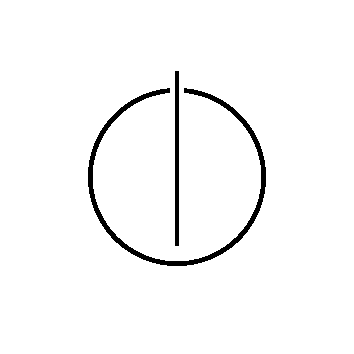
\includegraphics[width=4cm]{styles/informat.png}
  \end{figure}
   

\end{center}

% undo BCOR correction
\addtolength{\hoffset}{\bcorcor}
	
	
%	\input{components/cover_maschmeyer}
	\clearemptydoublepage
	
	% The titlepage for the CAMP report document.
% Included by MAIN.TEX


%--------------------------------------------------
% The title page
%--------------------------------------------------

% correct BCOR - undo at the end !!!
\def\bcorcor{0.15cm}
\addtolength{\hoffset}{\bcorcor}

\thispagestyle{empty}

 \vspace{10mm}
\begin{center}
	       \oTUM{4cm}
	   
	   \vspace{5mm}     
	   \huge FAKULT{\"A}T F{\"U}R INFORMATIK\\ 
	   \vspace{0.5cm}
	 \large DER TECHNISCHEN UNIVERSIT{\"A}T M{\"U}NCHEN\\
        
	\end{center}
		

\vspace{10mm}
\begin{center}

   {\Large \doctype}

  \vspace{10mm}
  
  {\LARGE \title}\\
  
  
  \vspace{10mm}
  
  
  {\LARGE  \titleGer}\\
  
  
  \vspace{10mm}

    %\hfill
    \begin{tabular}{ll}
	   \Large Author:     & \Large \author \\[2mm]
	   \Large Supervisor:    & \Large Prof. Dr. Hans-Arno Jacobsen \\[2mm]				
	   \Large Advisor:	& \Large M. Sc. Jan Adler\\[2mm]
	   \Large Date:       & \Large August 15, 2016
	 \end{tabular}
	 
	 \vspace{5mm}
	 
	 \begin{figure}[h!]
  \centering
   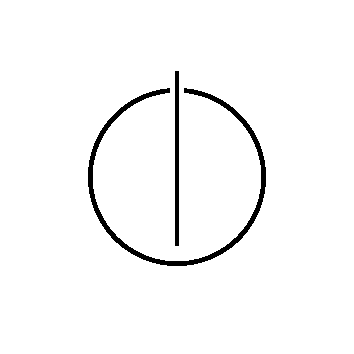
\includegraphics[width=4cm]{styles/informat.png}
  \end{figure}
   

\end{center}

% undo BCOR correction
\addtolength{\hoffset}{\bcorcor}
	
	
	\clearemptydoublepage


\thispagestyle{empty}
\selectlanguage{english}
	\vspace*{0.8\textheight}
	\noindent
	I assure the single handed composition of this master's thesis, only supported by declared resources.
	\newline
	\newline
	\newline
	\noindent
	M{\"u}nchen, August 15th, 2016 \hspace{5cm} \author
\selectlanguage{english}
\newpage
	
	\clearemptydoublepage
\phantomsection
\addcontentsline{toc}{chapter}{Acknowledgements}	


%\chapter*{Acknowledgements}

\vspace*{2cm}

\begin{center}
{\Large \bf Acknowledgments}
\end{center}

\vspace{1cm}

I would first like to thank my advisor Jan Adler for providing me the opportunity to work on an interesting topic and supervising me throughout the research. 
\newline

I thank Prof. Dr. Hans-Arno Jacobsen for providing me an opportunity to write my thesis under the Chair of Distributed Systems. I thank my advisor for providing me valuable feedbacks and suggestion from the start to the end of the thesis.
\newline

I would like to thank my family for giving me the motivation and moral support. I would also like to thank my friends Suvash Sedhain and Niroj Sapkota for their constant support and motivation. And special thanks to my friends for creating a positive environment by cracking jokes and taking off the pressure during coffee breaks.

	
	% Abstract for the TUM report document
% Included by MAIN.TEX


\clearemptydoublepage
\phantomsection
\addcontentsline{toc}{chapter}{Abstract}	





\vspace*{2cm}
\begin{center}
{\Large \bf Abstract}
\end{center}
\vspace{1cm}

% In today's world where billions of people exchange information online, service providers like Facebook, Twitter, Whatsapp store and process tremendous amount of data. Those service providers need distributed scalable storage systems to store and process big volume of data. Even though data are stored in a distributed storage systems, still the huge size of data are bottleneck for performance optimization. Scanning tens of millions rows and few million columns each time are expensive in terms of execution time and processing power. $Materialized$ $Views$ solve this problem by precomputing expensive queries and storing result in a physical table or disk. One of the bottleneck for this approach is constantly maintaining consistency between base table and view table. We propose a $Incremental$ $View$ $Maintenance$ approach to maintain consistency between base table and view table.


In today's world, billions of people exchange information online. Service providers like Facebook, Twitter, Whatsapp store and process tremendous amount of data. Those service providers need distributed scalable storage systems to store and process a big volume of data. Even though data are stored in a distributed storage systems, still the huge size of data can be a bottleneck regarding performance optimization. Scanning tens of millions of rows and few million columns each time are expensive regarding execution time and processing power. $Materialized$ $Views$ solve this problem by pre-computing expensive queries and storing the result in a physical table or disk. One of the bottlenecks for this approach is constantly maintaining consistency between the base table and the view table. In this thesis, we propose a $Incremental$ $View$ $Maintenance$ approach to maintain consistency between the base table and the view table.

	\tableofcontents
  
 % \clearemptydoublepage

\phantomsection
\addcontentsline{toc}{chapter}{Outline of the Thesis}

\begin{center}
	\huge{Outline of the Thesis}
\end{center}




%--------------------------------------------------------------------
\section*{Part I: Introduction and Theory}

\noindent {\scshape Chapter 1: Introduction}  \vspace{1mm}

\noindent  This chapter presents an overview of the thesis and it purpose. Furthermore, it will discuss the sense of life in a very general approach.  \\

\noindent {\scshape Chapter 2: Theory}  \vspace{1mm}

\noindent  No thesis without theory.   \\

%--------------------------------------------------------------------
\section*{Part II: The Real Work}

\noindent {\scshape Chapter 3: Overview}  \vspace{1mm}

\noindent  This chapter presents the requirements for the process.

	\mainmatter
	
	



\chapter{Introduction}
\label{chap:introduction}

Whenever we see our friends posting pictures on Facebook or Instagram, we like them or comment on them. Whenever we feel like sharing our thoughts, we either update status on Facebook or just tweet about it. If we need some relevant information, we just google it. The amount of data generated in such a fashion has to be stored somewhere. Companies like Facebook stores 500 TB of data each day\cite{daniel:datastats}, including 2.7 billion likes and 300 million photos. As of 2012, Facebook already has 100 petabytes of photos\cite{daniel:datastats}. Google, on the other hand, processes 3.5 billion requests per day \cite{daniel:datastats}. In the early 2000s, where there were fewer data shared on social media, data were stored in a relational database. Relational databases were designed in such a fashion to store a small amount of data and maintain integrity between them\cite{matt:rdb}. The amount of information we share on social media is expected to grow from 4.4 zettabytes in 2013 to 44 zettabytes in 2020(1 zettabyte is 1 trillion gigabytes)\cite{matt:rdb}. The scaling in RDBMS depends on adding more powerful CPU's and memory, i.e. only the vertical scaling is possible which is rather expensive.  One of the advantages of the big data storage system is that it can be scaled horizontally and is also useful for storing unstructured or semi-structured data. 

HBase is an open source sortedMap Datastore from Apache Software Foundation which is used as a database to store huge volume of data. HBase supports horizontal scalability, i.e. parts of a table can be put on several machines. This way a table is broken down into multiple pieces, thus making computation fast. But when we are talking about petabytes of data, scanning each part of the table for a single user query is still considered to be expensive regarding processing time. There are several techniques to reduce this effort, but we will be talking about $Materialized$ $Views$ approach. 



%In Chapter \ref{chap:background}, we analyse the fundamentals of views and view maintenance. In Chapter \ref{chap:relatedwork}, we present research, that is related to this thesis. In Chapter \ref{chap:analysis}, we define the requirements of the View Maintenance System and discuss possible alternatives.  In Chapter \ref{chap:architecture}, we align the architecture of the system and define its functionalities. In Chapter \ref{chap:viewconsistency}, we discuss threats to consistency and apply consistency techniques. In Chapter \ref{chap:loadbalancing}, we show how load balancing can be accomplished in the View Maintenance System. In Chapter \ref{chap:failuredetection}, we take counter measures to component failure. In Chapter \ref{chap:implementation}, we show challenges of the implementation. Finally, we evaluate and interpret the behaviour of the system in Chapter \ref{chap:evaluation}.\\%


\chapter{Background}
\label{chap:background}

In this chapter we will first discuss about the fundamentals of $Materialized$ $Views$ and $View$ $Types$. We will further explain about the technologies used widely in today's Distributed Storage Databases. 

\section{Materialized Views}

Materialized views are defined as the database object that stores the result of a query in a table or a disk. Materialized views are widely used for gaining performance advantage, i.e. to speed up query processing time over large datasets. The need for Materialized view addresses the problem of having to query large datasets that often needs joins and aggregations between multiple tables. These kind of queries are very expensive regarding execution time and processing power. Materialized views speed up the query processing time by pre-computing joins and aggregations before execution and stores these results in a table or disk\cite{materializedview:oracle}. 

\section{View Maintenance}
Once the Materialized views are created, our query is redirected to Materialized View table rather than base table. Whenever there is an update in the base table, the Materialized View table also has to be updated accordingly. One of the solutions would be recomputing the entire Materialized View from the scratch or using the heuristic of inertia\cite{maintenance:materializedviews} approach i.e. incremental maintenance with respect to the base table.

\section{Incremental Maintenance of Materialized View}
"A view V is considered consistent with the database DB if the evaluation of the view specification S over the database yields the view instance (V = S(DB)). Therefore, when the database DB is updated to DB0 , we need to update the view V to V0 = S(DB0) in order to preserve its consistency"\cite{incrementalmaintenance:materializedviews}. 

Recomputing Materialized view from scratch every time there is an update on base table is expensive. The other approach is to update the part of Materialized view table with respect to the update in Base Table. Our target is to maintain consistency between Materialized views and base table whenever there is an update on the base table.


\subsection{Aggregation}
In Aggregation view type, the data from the base table is merged on the basis of a particular key. In our implementation, we've implemented basic aggregation functions like sum, count, min and max. All these operations are carried out based on a particular key. So a unique key has sum, count, min and max operations. Whenever an update is triggered to update value for a particular key in the base table, in this case, count remains same and sum, min and max has to be recalculated. If a delete is triggered for a particular key in the base table, each of the aggregation functions has to be recalculated. 


\subsection{Join and Aggregation}
In Join and Aggregation case, we have at least two base tables. Joins being one of the complex structure itself, incremental view maintenance implementation involves a lot of complex cases. Here, to reduce complexity, we join two base tables on the basis of $key$ to form a new intermediate table. We group all the values of both base tables based on their keys. This way, for any update or delete trigger, the complexity of scanning whole base table is reduced to a single row. In our intermediate table, each of the base table is merged to a column family, join is applied and then result is stored in the view table. 

In the intermediate table, the unique keys from both the base tables act as the row key, both column families from base table are merged in the intermediate table. Now for a particular row key, the values are selected from base table and plotted in the intermediate table. Now join is applied between both column families of a particular row key, and sum of the join is inserted in the view table.  


\subsection{Join and Selection}
Join and Selection case is similar to the Join and Aggregation case, the only difference is instead of applying aggregation function, the join is applied for a particular row key and value is selected and inserted into the view table.

\newpage
\section{HBase}
\label{sec:hbase}

Before the evolution of HBase, Relational database systems were used particularly for storing and processing of data. Relational database systems have been used widely over a decade and are considered to be successful. In a relational database, multiple tables are used to store different types of data, this segregation of data gives more clear and systematic view of the data\cite{relational:dbs}. However, one of the biggest drawbacks in Relational database is the difficulty of scaling horizontally. The major disadvantage of relational database design is the performance if the number of tables between which the relationships has to be defined is large, i.e. more operation power needed for computation\cite{relational:dbs}. 

HBase is an open source sortedMap Datastore from Apache Software Foundation. HBase is modelled after Google's BigTable framework. It is a Hadoop database that is used for storing and retrieving data with random access. HBase architecture is designed to run on a cluster of computers rather than a single machine \cite{coprocessor:detail}. HBase aims to scale horizontally by adding more machines to the cluster. HBase runs on top of HDFS(Hadoop Distribution File System) that provides the functionality alike of Google's Big Table and provides a fault-tolerant way of storing a large volume of semi-structured and unstructured data\cite{bigdata:analysis}.

HBase is built on top of Hadoop and Zookeeper\cite{coprocessor:detail}. Both Hadoop and Zookeeper are open source projects from Apache Software Foundation. Apache Hadoop is an open source framework that facilitates storing and processing large dataset in a distributed fashion. Zookeeper, which was developed under Apache software foundations, as a sub-project of Hadoop, is an open source distributed configuration service for large distributes applications. A basic table structure of HBase consists of Row Key, which is similar to the primary key in a relational database table, Column Family and Column Qualifier. The figure below describes a HBase table and it's mapping to the relational database table.


\begin{figure}
	\centering
	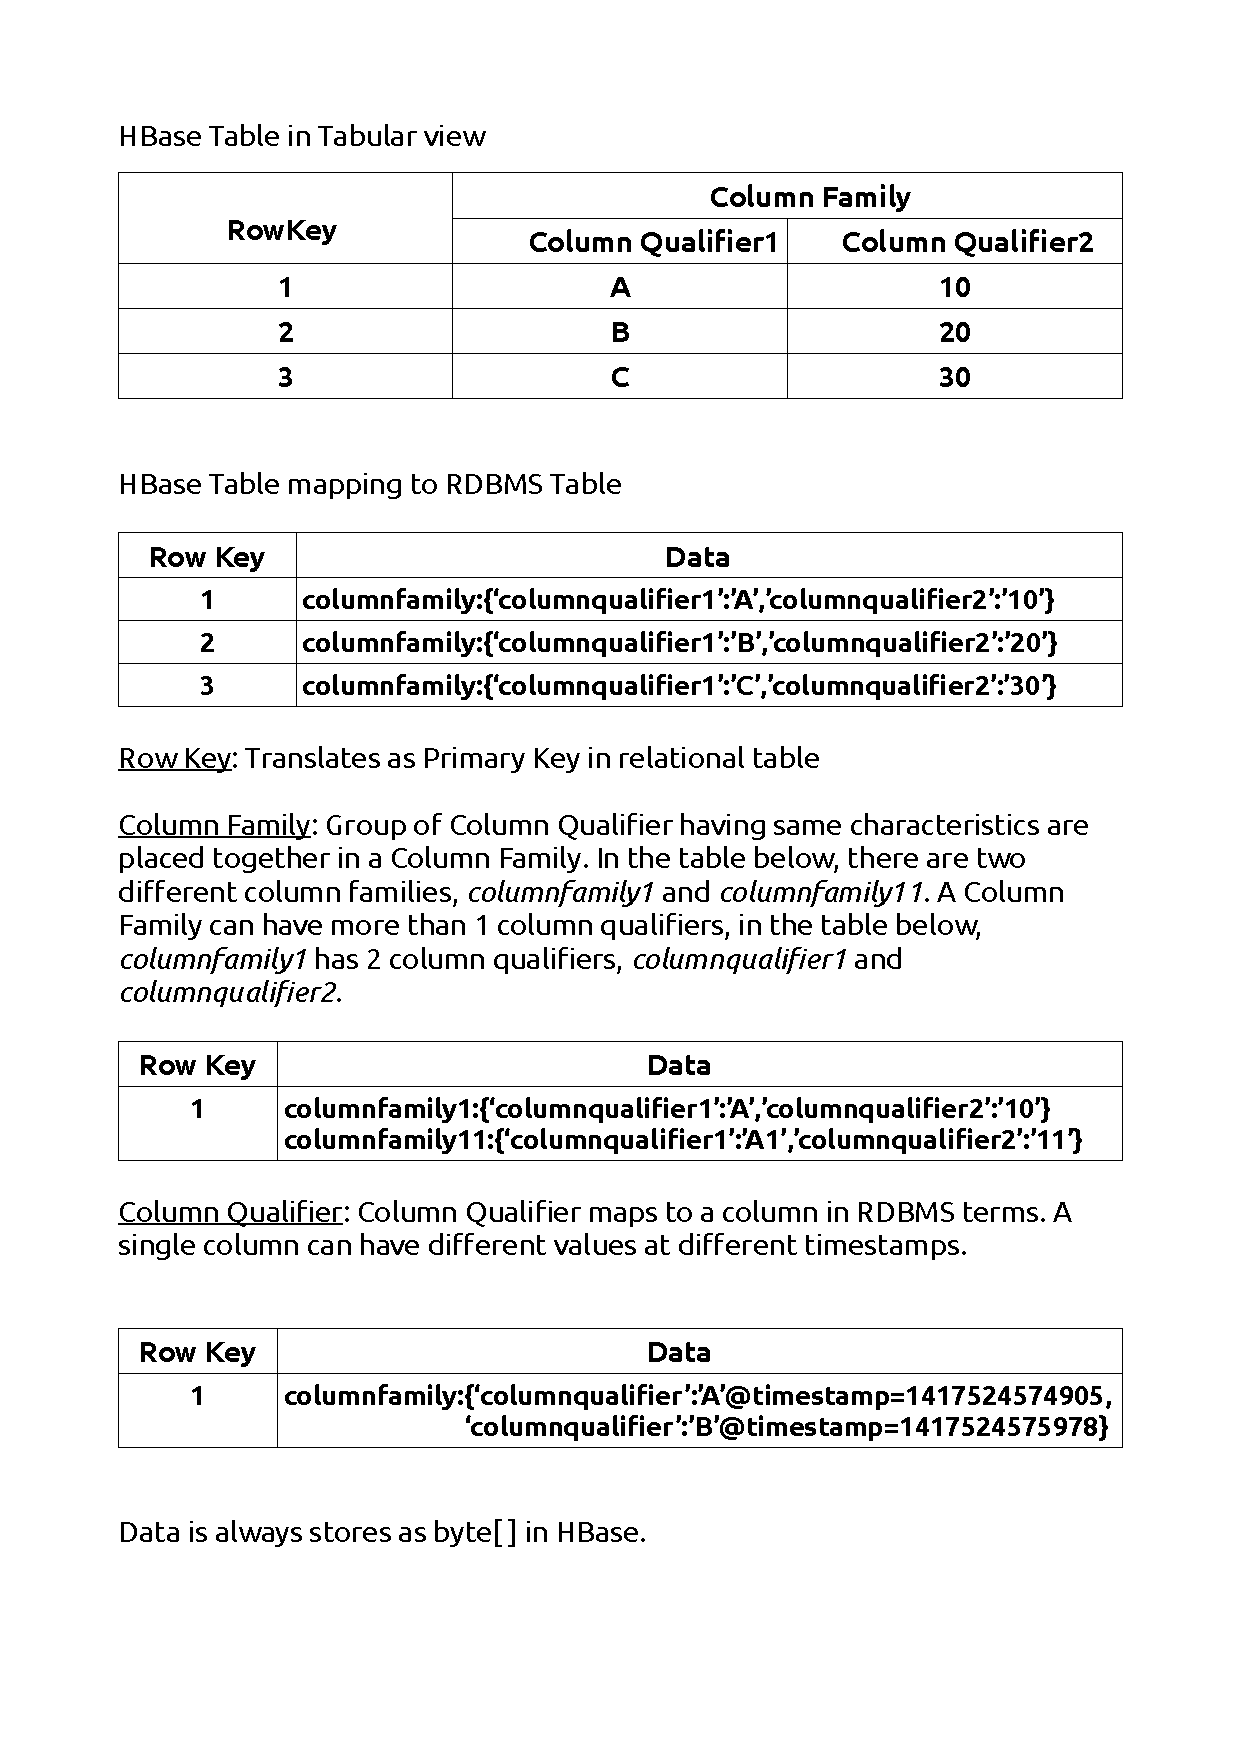
\includegraphics[width=\linewidth]{HBase}
	\caption{HBase Table}
	\label{fig:hbasetable}
\end{figure}

\newpage
\subsection{HBase Architecture}
\label{HBase Architecture}
HBase architecture consists of three major components and three sub components. The major components are Master, Region server and zookeeper. The three sub components are Write-Ahead-Log(WAL), HFile and Memstore\cite{hbase:insights}. HBase architecture is based on Master-Slave architecture, where the Master is known as HMaster, is the master node and Region Servers are the slave nodes. Whenever the write request is sent, HMaster receives the request and forwards it to the respective Region Server\cite{hbase:insights}. 

\subsubsection{HMaster}
\label{hmaster}
HBase Master is mainly responsible for region assignments within the region servers and DDL operations like creating and deleting tables\cite{hbase:architecture}. Apart from these roles, HMaster is also responsible for assigning the regions and re-assigning of the regions for recovery or load balancing\cite{hbase:architecture}. HMaster also monitors all the instances of Region Servers in the cluster\cite{hbase:architecture} and mainly provides administrative operations.

\subsubsection{Region Servers}
\label{region serves}
Region servers are systems within HBase that acts like a data node\cite{hbase:insights}. When a HMaster receives a write request, it forwards the request to the Region Server. Region server can have multiple regions within it, and it directs the request to the specific region. Region servers are mainly responsible for handling data related operations and communication. Region servers handle the read/write request for all the regions within it. 
A Region Server runs on data node and it has four sub components as described below\cite{hbase:architecture}
\begin{description}
	\item[$\bullet$]  Write Ahead Log(WAL): Write Ahead Log is basically a log file. Region server adds each request to WAL first before sending that request to the appropriate region. It is mainly used for recovery in case of failure\cite{hbase:insights}. If the request is not written in the WAL file, there is a possibility of data loss in case of Region Server failure.
\end{description}

\begin{description}
	\item[$\bullet$]  BlockCache: BlockCache is the read cache that is used to store frequently read data\cite{hbase:insights}. When the cache is full, last read data is removed from the cache.
\end{description}

\begin{description}
	\item[$\bullet$] MemStore: MemStore is the write cache. All the new data that has not been written to the disk are stored in MemStore. It is mainly responsible for keeping tracks of all the logs for read and write operations to be performed for a specific Region Server\cite{hbase:architecture}. Each column family in a region has one MemStore\cite{hbase:insights}.
\end{description}

\begin{description}
	\item[$\bullet$] HFile: In HBase, column family is a collection of multiple HFiles. HFiles are used to store rows as keyValue pairs and are immutable and sorted\cite{hbase:insights}.
\end{description}

\subsubsection{Zookeeper}
\label{zookeeper}
Zookeeper an open source project under Apache Software Foundations, is a distributed software system that provides a infrastructure for synchronization across the clusters. It provides coordination between distributed processes across the cluster so that client receives consistent data. The architecture of Zookeeper is based on client-server model. The client acts as a node that make use of the service and server acts as a node that provides the service\cite{hbase:zookeeper}. Many Zookeeper servers can be collected together, that is known as $Zookeeper$ $ensemble$\cite{hbase:zookeeper}. Each server node of the zookeeper at a given time can handle large number of client connections. It is essential to know if the connection is alive, so the client node sends a ping request to the server it is connected to make sure it is connected and alive\cite{hbase:zookeeper}. The server, after receiving ping request, sends an acknowledgement to indicate that server is alive. If the client doesnot receive acknowledgement within a given specific time, then the client connects to another zookeeper server within a $Zookeeper$ $ensemble$ and the client session is transferred to the new zookeeper server\cite{hbase:zookeeper}.
\newline
HBase has a tight integration with Zookeeper. HBase uses Zookeeper as a distributed coordination service to facilitate synchronization between the servers in a cluster. HBase also uses Zookeeper to keep track of state of the servers, which servers are alive and available\cite{hbase:architecture}. Whenever a HBase instance is started, it automatically starts Zookeeper instance, as Zookeeper comes integrated with HBase\cite{hbase:insights}. Zookeeper is used to keep tracks of the number of regions servers available, and the data hold by each region servers. 
\newline

The figure below explains the HBase Architecture and its components.
\begin{figure}
	\centering
	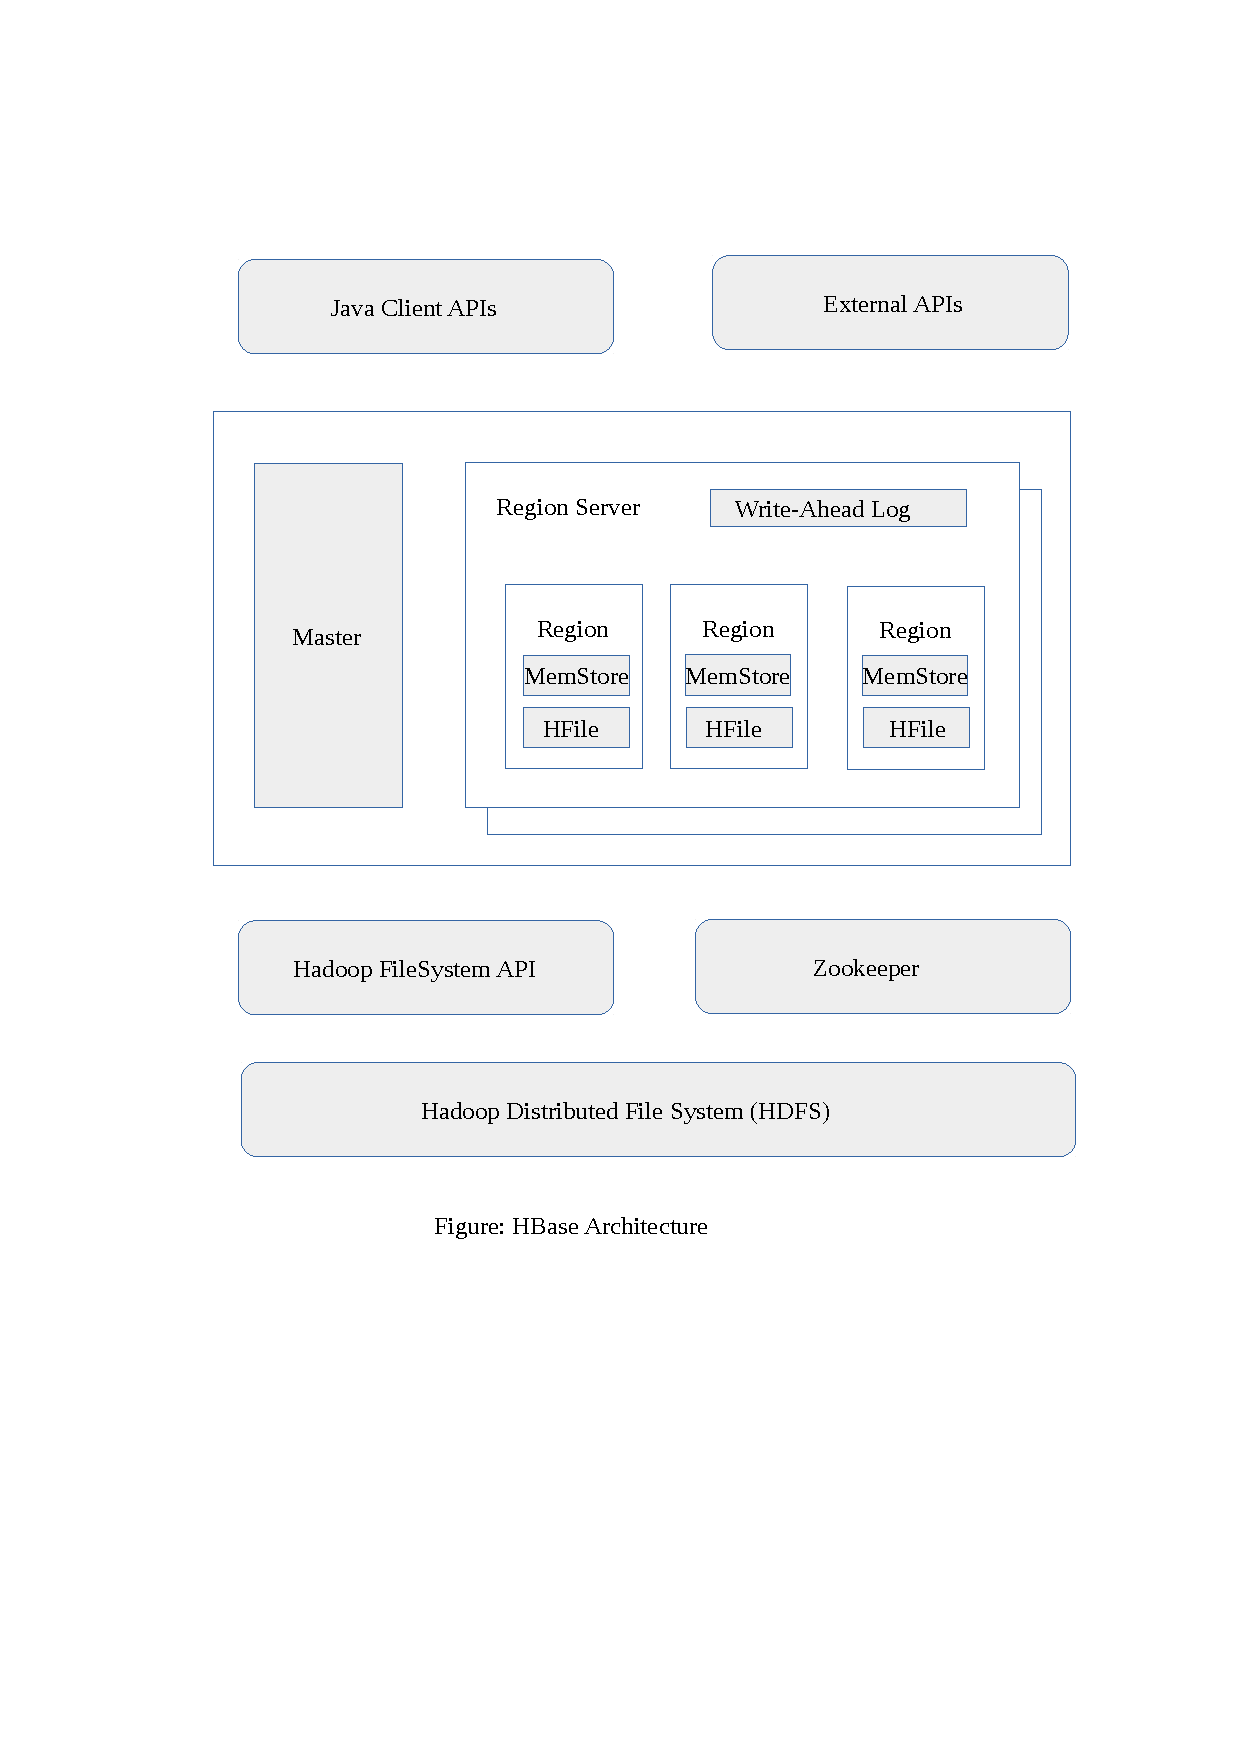
\includegraphics[width=\linewidth]{HBase_Architecture}
	\caption{HBase Architecture}
	\label{fig:hbasetable}
\end{figure}

\newpage
\section{Hadoop Distributed File System}
\label{Hadoop Distributed File System}


\newpage
\section{Coprocessor}
\label{sec:coprocessor}

HBase Coprocessor framework provides a library to run user code in the HBase Region Server. The advantage of this framework is that it decreases the communication overhead of transferring the data from HBase region server to the client, thus improving the performance by allowing the real computation to happen in the HBase region server\cite{coprocessor:coprocessor}. There are two types of coprocessor, Observer coprocessor  which acts more like relational database triggers and Endpoint coprocessor that resembles stored procedures of RDBMS\cite{coprocessor:types} 


\subsection{Observer coprocessor}
\label{sec:observercoprocessor}
Observer coprocessor as stated earlier, is more like database triggers that executes our code when certain events occur. In the figure below, we first try to explain a simple life cycle of put() operation as an example\cite{coprocessor:detail}. Observer coprocessor resides between the client and the HMaster. Observer coprocessor can be triggered after every get(), put() or delete() command. The CoprocessorHost class is responsible for observer registration and execution\cite{coprocessor:detail}.  During the life cycle of events, Observer coprocessor allows us to hook triggers in two stages. The first one is before the occurrence of the event and the other is after the completion of the event. For example, if we want to perform some computations before the occurrence of put event, we can use prePut() method to perform our custom computation. Then the life cycle of put event starts and after the life cycle of put event is completed, we can use postPut() method to perform custom computation. In the figure below, we try to explain the lifecycle of observer coprocessor when a put event is fired\cite{coprocessor:detail}.
\newline
There are four types of Observer Interfaces provided as of HBase version 1.1.3\cite{hbase:essential}.

\begin{enumerate}
    
\item RegionObserver: RegionObserver runs on all the Region of a HBase table. RegionObserver provides hook for data manipulation for events like put(), get() add delete() events. All the data manipulations are done with pre-hook and post hook\cite{hbase:essential} such as pre and post observers. For instance, preGetOp() and postGetOp() provides hook for manipulating get request. 

\item RegionServerObserver: Likewise in RegionObserver, RegionServerObserver provides a hook for data manipulation for events like merge, commits and rollback. All the data manipulation are done with pre-hook and post hook such as preMerge() and postMerge(). 

\item WALObserver: WALObserver interface provides a hook for Write-Ahead-Log(WAL)\cite{hbase:essential} related operations. This interface provides only preWALWrite() which is triggered before WALEdit is written to Write-Ahead-Log and postWALWrite() which is triggered after WALEdit is written to a Write-Ahead-Log.

\item MasterObserver: MasterObserver Interface provides a hook for data manipulation for DDL events such as table creation, table deletion or table modification\cite{cloudera:instandupg}. For instance, if the secondary indexes need to be deleted when primary table is deleted, we can use postDeleteTable(). The MasterObserver runs on the master node.

\end{enumerate}

\begin{figure}
    \centering
    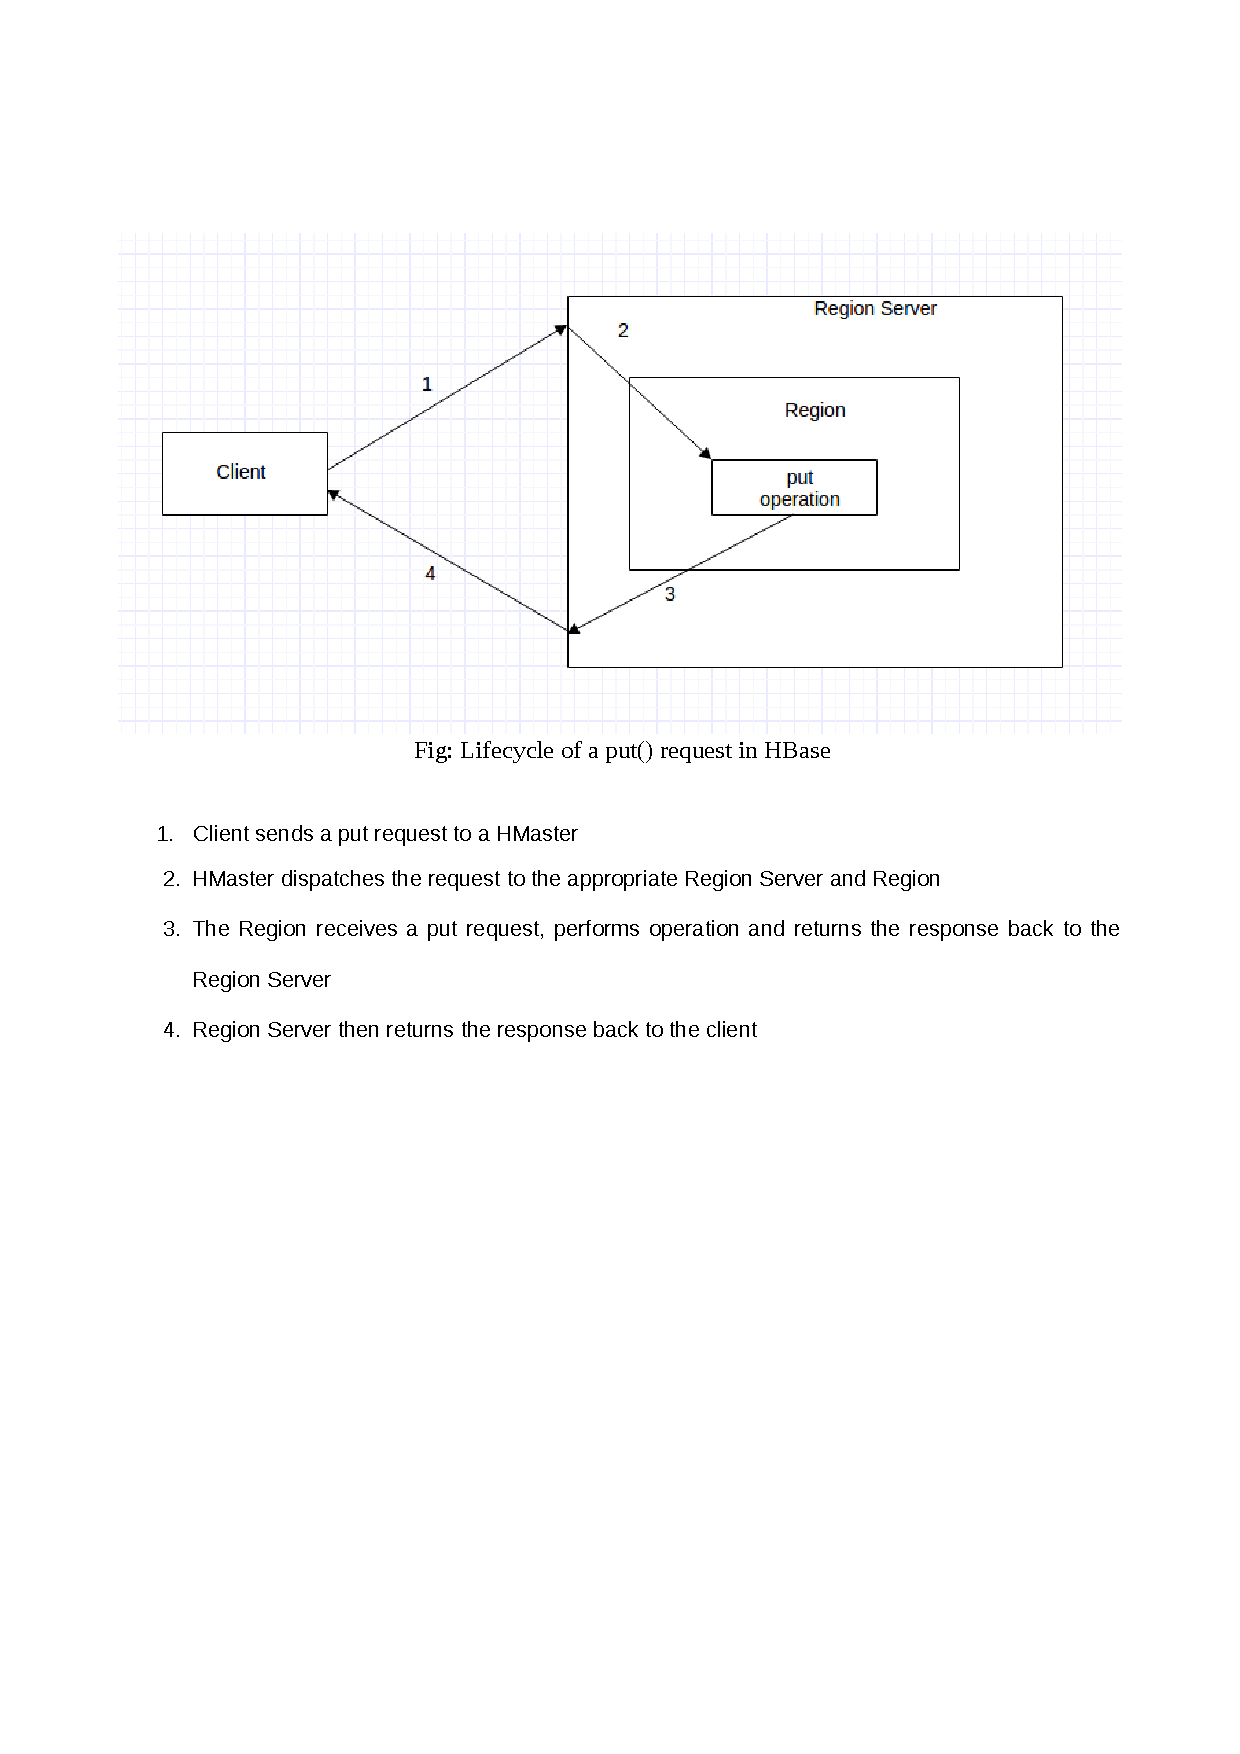
\includegraphics[width=\linewidth]{PutRequestLifeCycle}
    \caption{Life cycle of put request}
    
\end{figure}

In the figure below, We can see the life-cycle of a put request with observer coprocessor implemented.

\begin{figure}
    \centering
    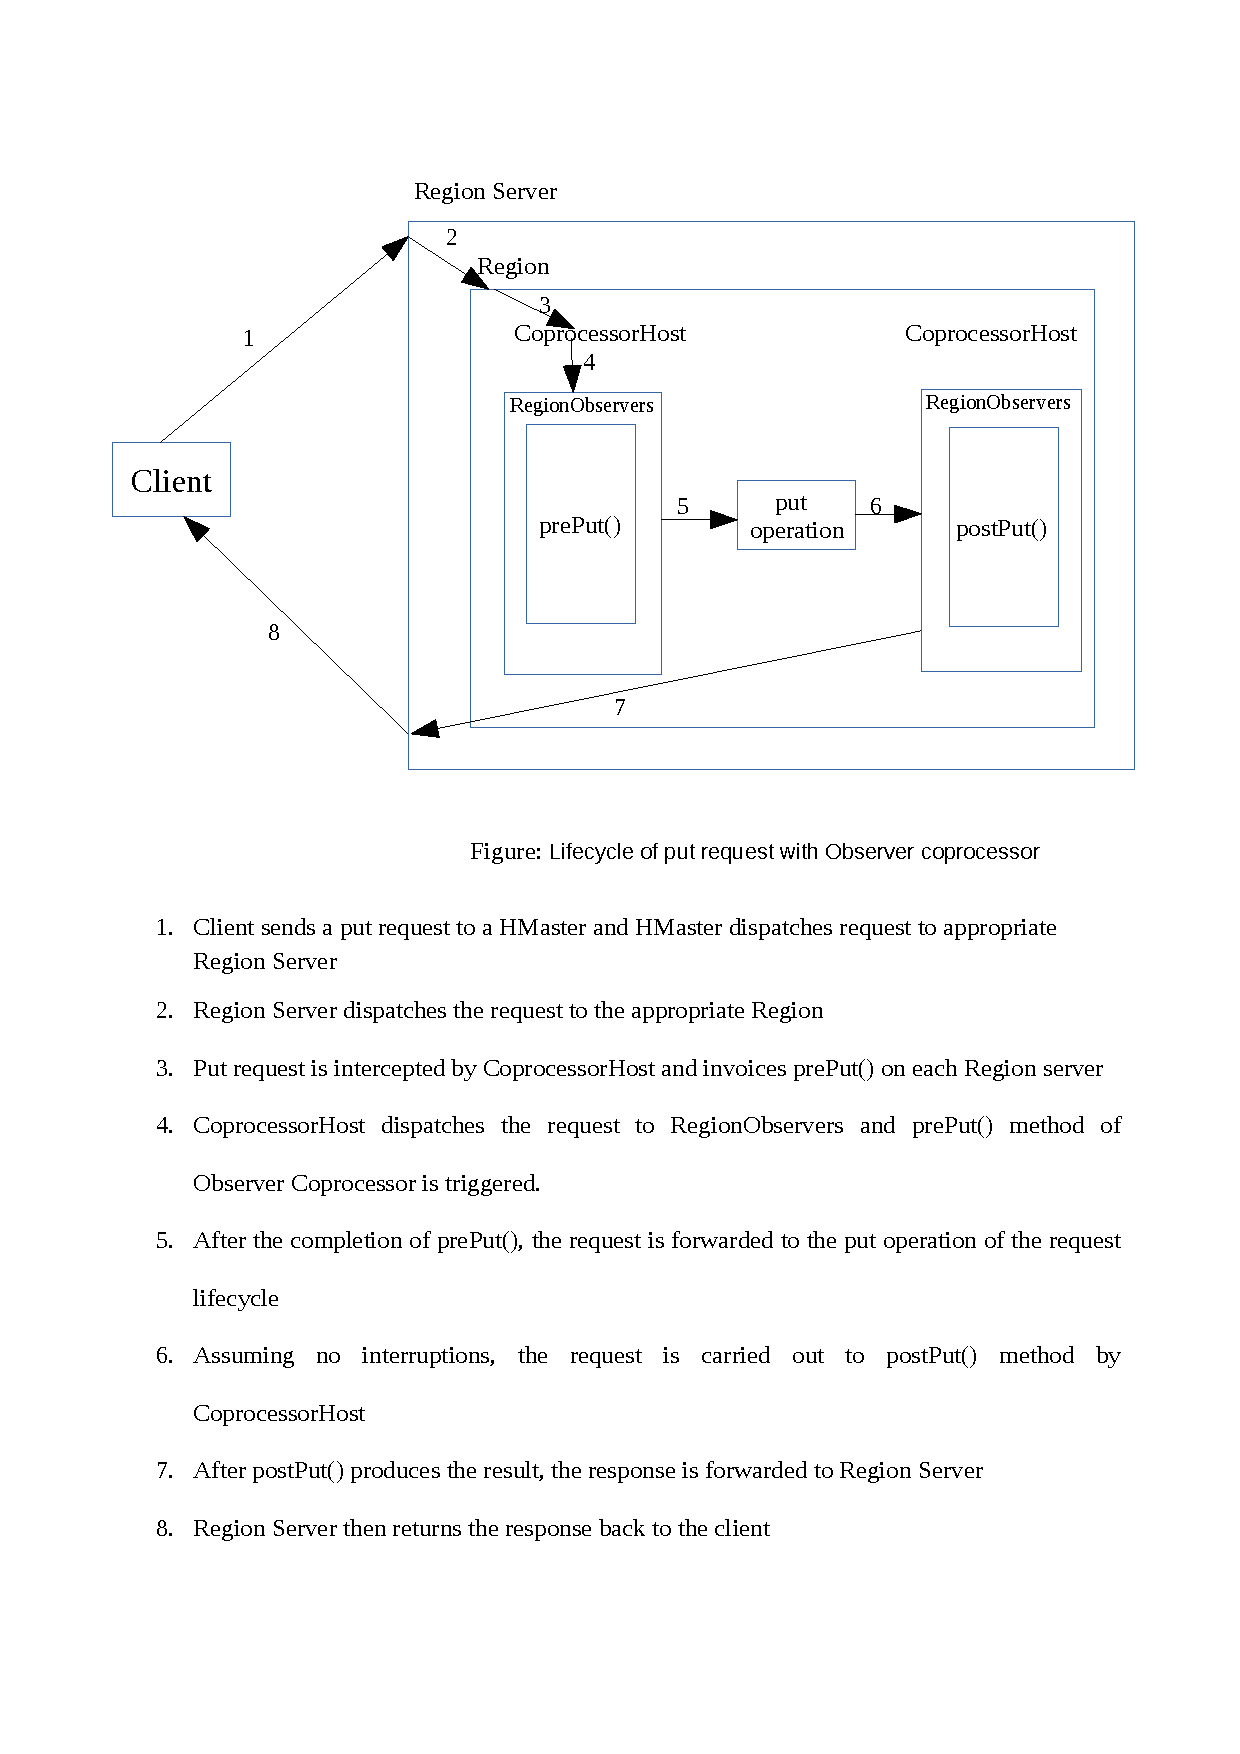
\includegraphics[width=\linewidth]{PutRequestWithObserverCoprocessor}
    \caption{Life cycle of put request with observer coprocessor}
    
\end{figure}

\newpage
\subsection{Endpoint coprocessor}

Endpoint coprocessor is similar to the Stored Procedures in RDBMS. This type of coprocessor is more useful in the scenario where the computation is needed for the whole table and are not provided by observer coprocessor\cite{hbase:coprocessors}. Invoking the endpoint coprocessor is similar to invoking any other commands in HBase from the client\textquotesingle s point of view but the result is based on the code that defines the coprocessor\cite{coprocessor:detail}. The figure below explains the Aggregation example\cite{coprocessor:detail}.

\begin{figure}
    \centering
    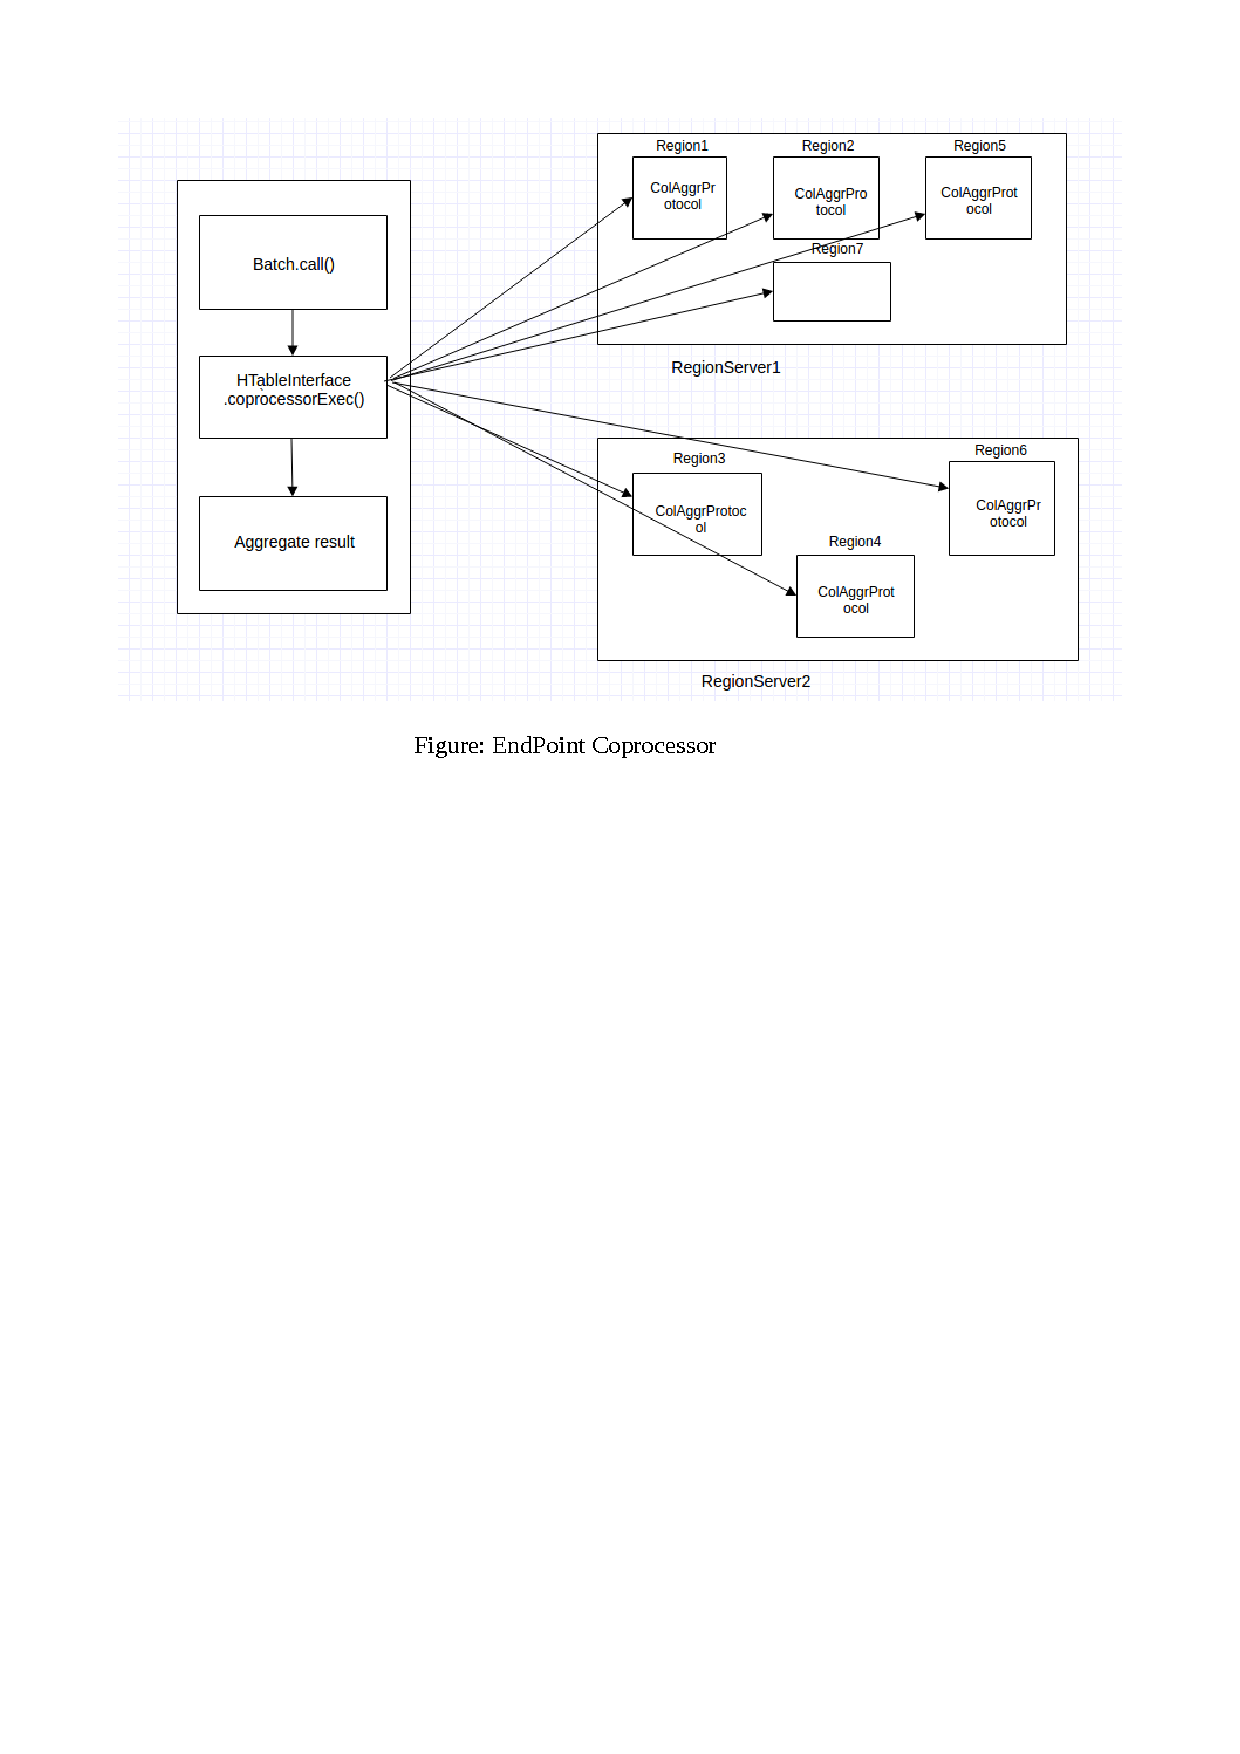
\includegraphics[width=\linewidth]{EndPointCoprocessor}
    \caption{EndPoint Coprocessor}
    
\end{figure}

When a request is invoked from a client, an instance of Batch.call() encapsulates the request invocation and the request is forwarded to coprocessorExec() method of HTableInterface. Then the coprocessorExec() handles the request invocation and distributes the request to all the Regions of the RegionServer. Assuming that no interruptions occurs and all the requests are completed, the results is then returned to client and aggregated\cite{coprocessor:detail}.


\newpage
\chapter{Implementation}
In this section, we will first discuss the prerequisite of implementation and then the proposed method for our research.

\section{Prerequisite}
Before we begin with our implementation of the coprocessor, there are few steps to load coprocessor into our HBase table. The coprocessor can be loaded to the base tables in two ways: statically and dynamically\cite{loading:coprocessors}. 

\subsection{Static Loading of coprocessor}
We have to define coprocessor properties in a $hbase$-$site.xml$ file inside a \textless property\textgreater \space element followed by \textless name\textgreater \space and a \textless value\textgreater \space sub element. The \textless name\textgreater \space sub element should have one of the followings\cite{hbase:site}:

\begin{enumerate}
    \item hbase.coprocessor.region.classes for RegionObservers and Endpoints coprocessor
    \item hbase.coprocessor.wal.classes for WALObservers
    \item hbase.coprocessor.master.classes for MasterObservers
    
\end{enumerate}

The \textless value\textgreater \space sub-element should contain the full path of the coprocessor implementation class. A typical example for static loading of coprocessor looks as,\newline \newline \textless property\textgreater \newline
\textless name\textgreater hbase.coprocessor.region.classes\textless /name\textgreater \newline
\textless value\textgreater \texttt{org.apache.hbase.HBase\_coprocessor.HBaseCoprocessor}\textless /value\textgreater \newline
\textless /property\textgreater \newline

 If we have multiple classes, then the path in \textless value\textgreater \space sub-element should be comma separated. In this setup, the framework will attempt to load all the configured classes, so we have to create a jar with dependencies, for all the classes and place the location of the jar to HBase classpath. For that, we have to export /path/to/jar in $hbase$-$env.sh$ file. A typical example for exporting classpath is given below, \newline \newline
 export \texttt{HBASE\_CLASSPATH}='/path/to/jar' \newline
 
Now if HBase is restarted without any errors, we have managed to load system coprocessor successfully. 

\subsection{Static Unloading of coprocesssor}
\begin{enumerate}
    \item Delete entry from $hbase$-$site.xml$
    \item Delete entry for $hbase$-$env.sh$
    \item Restart HBase
\end{enumerate}

\subsection{Dynamic Loading of coprocessor}
In this approach, rather than loading coprocessor to all the tables in a Region, the coprocessor is loaded to specific tables of the region. There are two implementations of loading coprocessor dynamically, from HBase shell or using Java API\cite{hbase:site}.

\subsubsection{Using HBase shell}
\begin{enumerate}
	\item disable table \newline
			\space \space hbase\textgreater disable '\textless \texttt{table\_name}\textgreater'
	\item load coprocessor using the following command \newline
	alter '\textless \texttt{table\_name}\textgreater', \newline 
	METHOD =\textgreater '\textless \texttt{table\_att}\textgreater', 'coprocessor' =\textgreater '/file/to/path\text{\textbar}\newline/source/path/to/impementation/class\text{\textbar}1001\text{\textbar}'
	\newline \newline
	A typical example looks like,\newline \newline
	alter 'BaseTableA', METHOD =\textgreater '\texttt{table\_att}', 'coprocessor' =\textgreater 'file:///home/saroj-gautam/Documents/HBase-coprocessor-0.0.1-SNAPSHOT-jar-with-dependencies.jar\text{\textbar}\texttt \newline {org.apache.hbase.HBase\_coprocessor.HBaseCoprocessor}\text{\textbar}1001\text{\textbar}'
	
	\item enable table \newline
	See if coprocessor is loaded successfully. We can see it by seeing the table properties. \newline 
	hbase\textgreater describe '\textless \texttt{table\_name}\textgreater \space should list the coprocessor under \texttt{TABLE\_ATTRIBUTES.} \newline

\end{enumerate}

In the above scenario, the coprocessor tries to read class information from \texttt{table\_att} property. There are certain arguments separated by pipe (\text{\textbar}). The first argument in the value is the file path to the jar file that contains the implementation class. The second argument contains the full classname of the implemented coprocessor. The last argument represents the execution sequence of registered observers. If this field is left blank, the framework will itself assign a default priority value\cite{hbase:site}.

\subsubsection{Using Java API}
Prior to HBase version 0.96, the coprocessors were loaded in a different way. After HBase version 0.96 and newer, HTableDescriptor class provides addCoprocessor() method that helps to load coprocessor in an easier way. A code snippet\cite{loading:coprocessors} below will give us a basic insight of how coprocessor is loaded dynamically from Java API in older versions and newer versions of HBase.
\newline \newline
\textbf{Older than 0.96} \newline
\lstset{language=Java}
\begin{lstlisting}
String path = "/path/to/jar"
admin.disableTable(<table_name>)
hTableDescriptor.setValue("COPROCESSOR$1", path + "|"
    + RegionObserverExample.class.getCanonicalName() + "|"
    + Coprocessor.PRIORITY_USER);
admin.enableTable(<table_name>)
\end{lstlisting}

\textbf{0.96 or newer} \newline
\lstset{language=Java}
\begin{lstlisting}
String path = "/path/to/jar"
admin.disableTable(<table_name>)
hTableDescriptor.addCoprocessor(<class_name>.class.getCanonicalName(),
             path, Coprocessor.PRIORITY_USER, null);
admin.enableTable(<table_name>)
\end{lstlisting}

\subsection{Dynamic Unloading of coprocessor}
Dynamic unloading of coprocessor can also be done in two ways, from shell and from Java API. 

\subsubsection{Using HBase shell}
\begin{enumerate}
    \item disable table
    hbase\textgreater disable '\textless \texttt{table\_name}\textgreater'
    \item alter table, remove coprocessor
    hbase\textgreater alter '\textless \texttt{table\_name}\textgreater', \newline
    METHOD =\textgreater '\texttt{table\_att\_unset}', NAME=\textgreater 'coprocessor\$1' =\textgreater
    \item enable table
    hbase\textgreater enable '\textless \texttt{table\_name}\textgreater'
     
\end{enumerate}

\subsubsection{Using Java API}
Using Java API, in the newer version we can use removeCoprocessor() method provided by HTableDescriptor class and in the older version, we can use setValue() to unload coprocessor.

\section{Proposed Method}
In this section, we will explain about the algorithms we've implemented to maintain incrementally materialized views for 
\begin{enumerate}
    \item Aggregation
    \item Join and Aggregation
    \item Join and Selection
\end{enumerate}

One of the most important features in our implementation is the introduction of intermediate table. We have introduced intermediate table in order to restrict the scanning of the entire base table for a simple get, put or delete operation. Scanning billions of rows for such operations can be expensive in terms of processing power and CPU usage. 

\subsubsection{Creation of Intermediate table}
\label{subsec:intermediatetable}

If there are two base tables, then we merge column families of both tables into the intermediate table. If there is only one base table, then we have the same column family in our intermediate table. The $key$ from base table becomes row key for the intermediate table, $row key$ of the base table becomes $column$ $qualifier$ in the intermediate table. So the value for key and row key from base table is now plotted in intermediate table for that particular key. So whenever there is a CRUD operation for a particular key, we can scan row for the particular key instead of scanning the whole table. The figure below explains the transformation of base table into an intermediate table in more detail. 

\begin{figure}
    \centering
    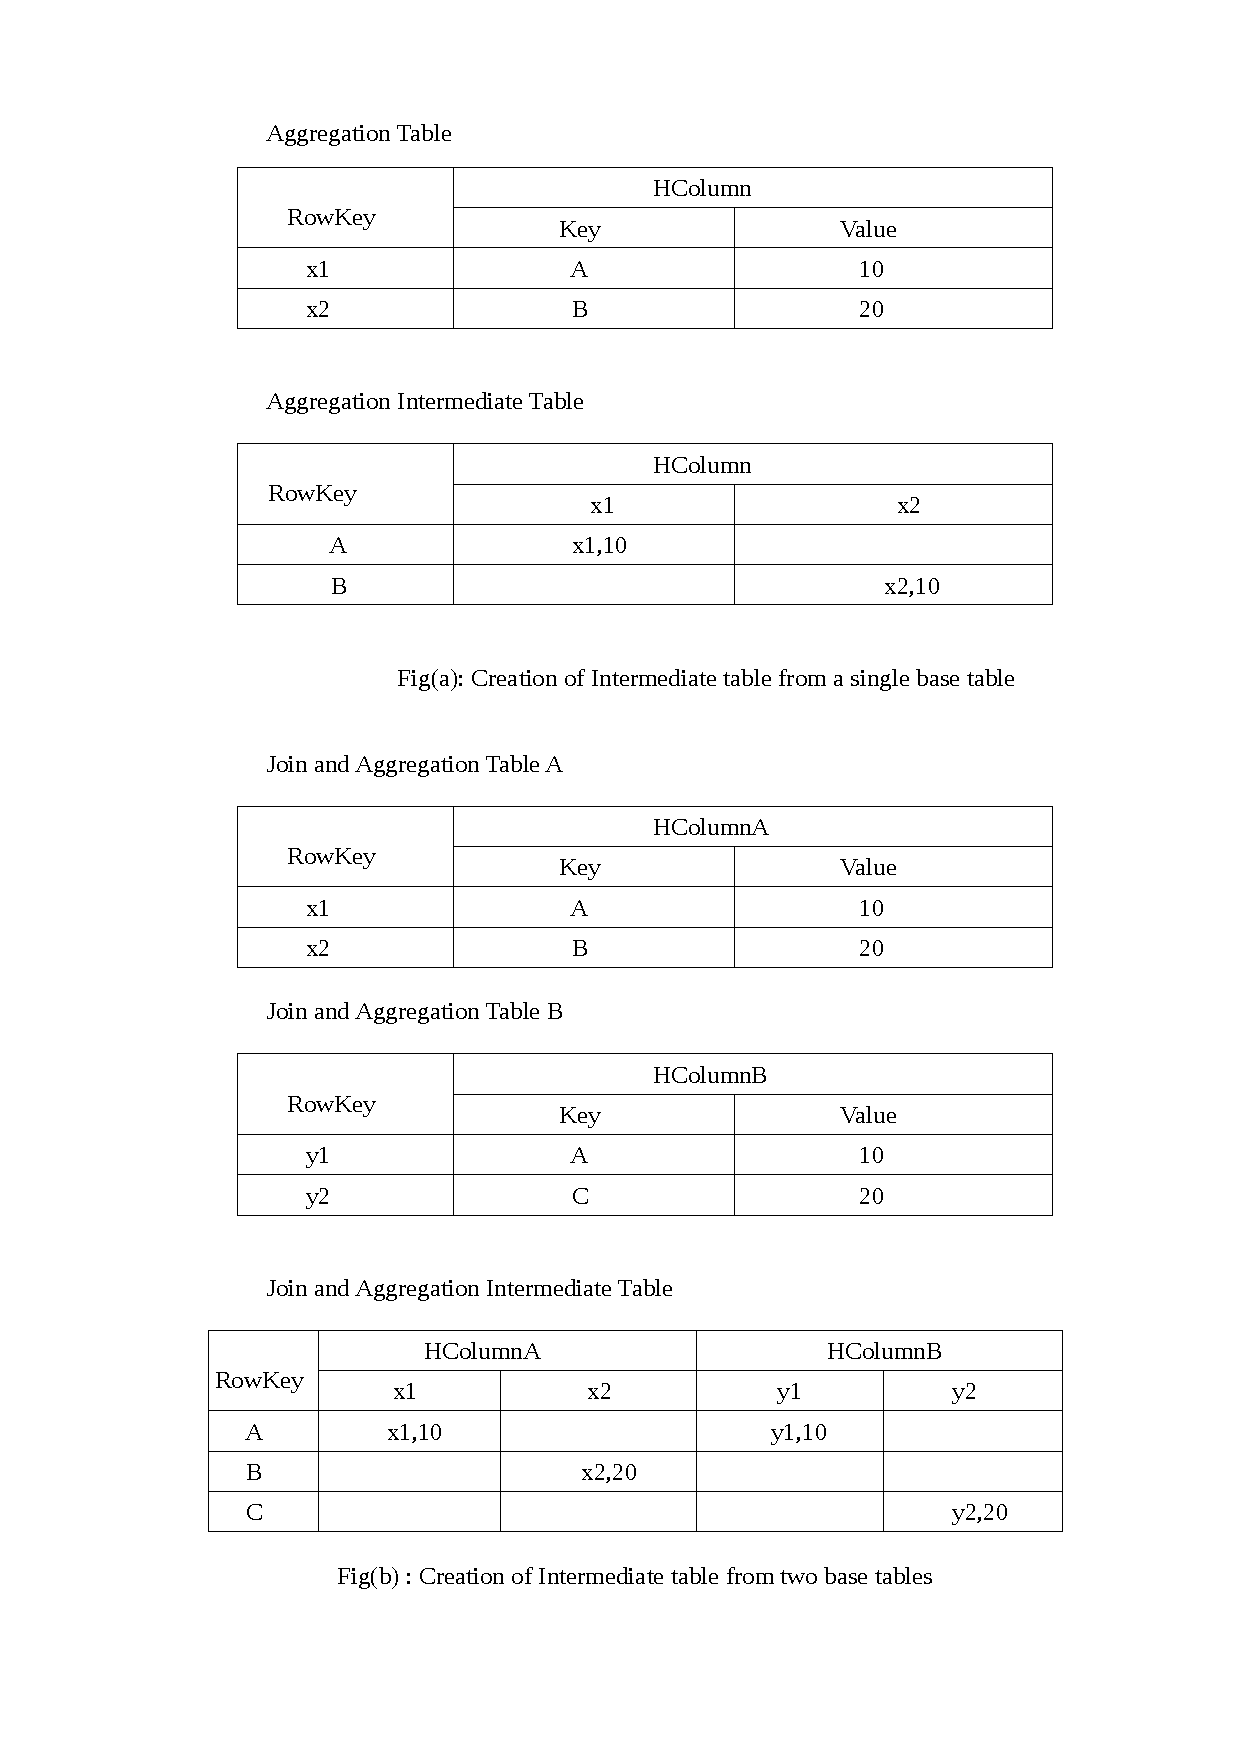
\includegraphics[width=\linewidth]{IntermediateTable}
    \caption{Intermediate Table}
    
\end{figure}

\newpage
\subsection{Aggregation}
\label{sec:aggregationImpl}

In our implementation, we've implemented basic aggregation functions like sum, count, min and max. All these operations are carried out based on a particular key. The base table contains key,value pairs. We construct an intermediate table from the base table. The reason behind constructing intermediate table is to restrict scanning of the whole base table for an update/delete trigger for a particular key in a base table. We take the unique keys and map them as a row key in the intermediate table, and accordingly the values are plotted. Once all the values are plotted in the intermediate table, we then construct view table. The view table contains aggregate functions like Sum, Count, Min and Max for each row Key i.e. for each unique keys of the base table. 

%The figure below explains how we map base table to a view table.

%\begin{figure}
%    \centering
%    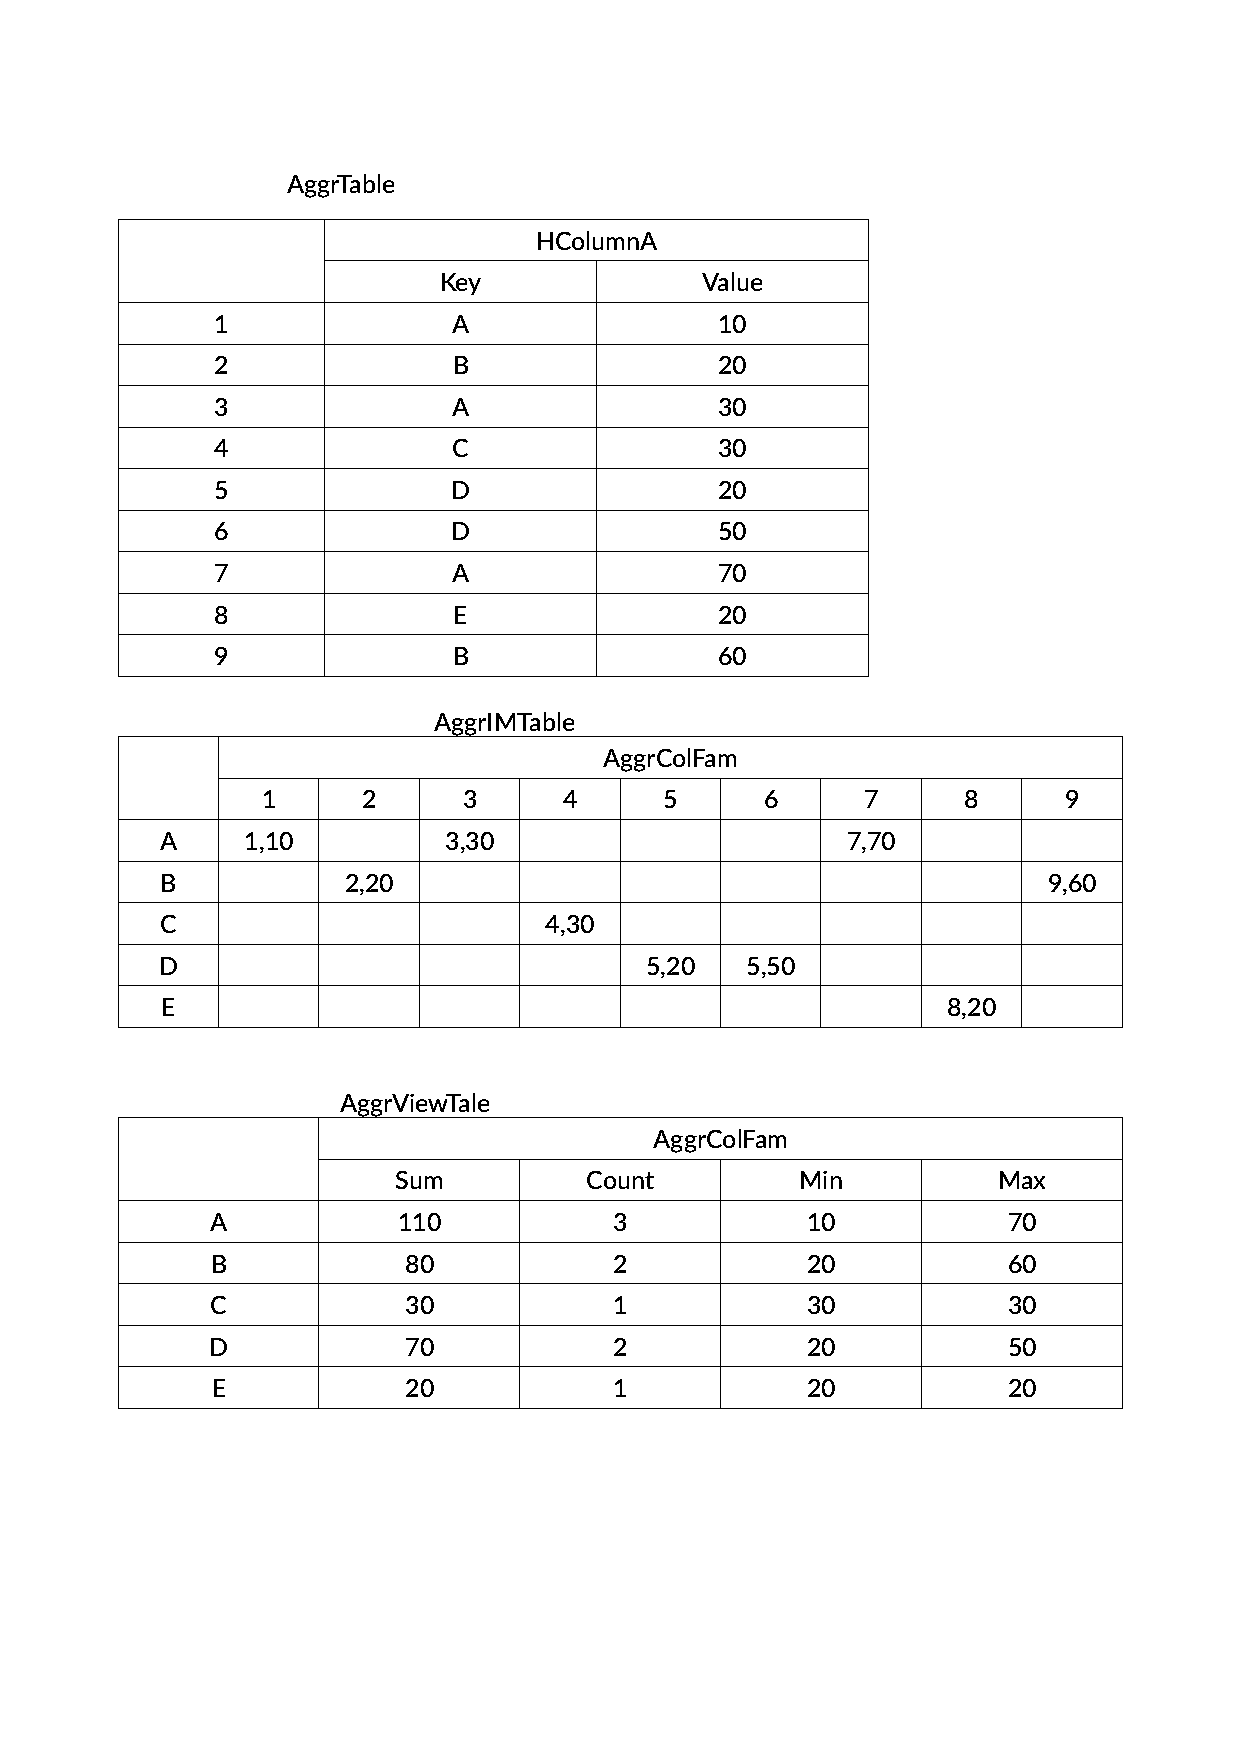
\includegraphics[width=\linewidth]{Aggregation}
%    \caption{Aggregation}
%    \label{sec:aggregation}
    
%\end{figure}
%\newpage

Once we have a base table, intermediate table and view table, and successfully loaded coprocessor on our base table, we are ready to go ahead with our implementation. There are certain scenarios where coprocessor is triggered for an update and delete operations.

\begin{enumerate}
    \item New row is inserted
    \item Existing value of a row is updated
    \item Existing key of a row is updated
    \item Existing row is deleted
\end{enumerate}

\subsubsection{New row is inserted}
Whenever a new row is inserted in a base table with (key,value) pair, the (key,value) pair has to be inserted in the base table and we have to plot the new (key,value) pair in the intermediate table and also view table has to be updated accordingly. Using prePut() and postPut() triggers from observer coprocessor, we perform all the required operations.

As we have already discussed put() request life cycle in \ref{sec:observercoprocessor}, before the (key,value) is inserted, we catch the request using prePut() method provided by the observer coprocessor. In the prePut() method, we verify the inputs and check if new row is inserted or existing row is updated. After we verify that new row is being inserted, we let the request to insert new (key,value) pairs to be inserted into the base table. After new (key,value) pair is inserted into the base table, we again catch the request in postPut() method. In postPut() method, we plot the (key,value) pair in the intermediate table and then update aggregation functions in our view table. The figure below explains the scenario when a new row is inserted. The left side tables are the default tables and right side tables explain the behavior when a new row is inserted. The text displayed in red mark the changes that are happening on base table, intermediate table and view table. 
\begin{figure}
    \centering
    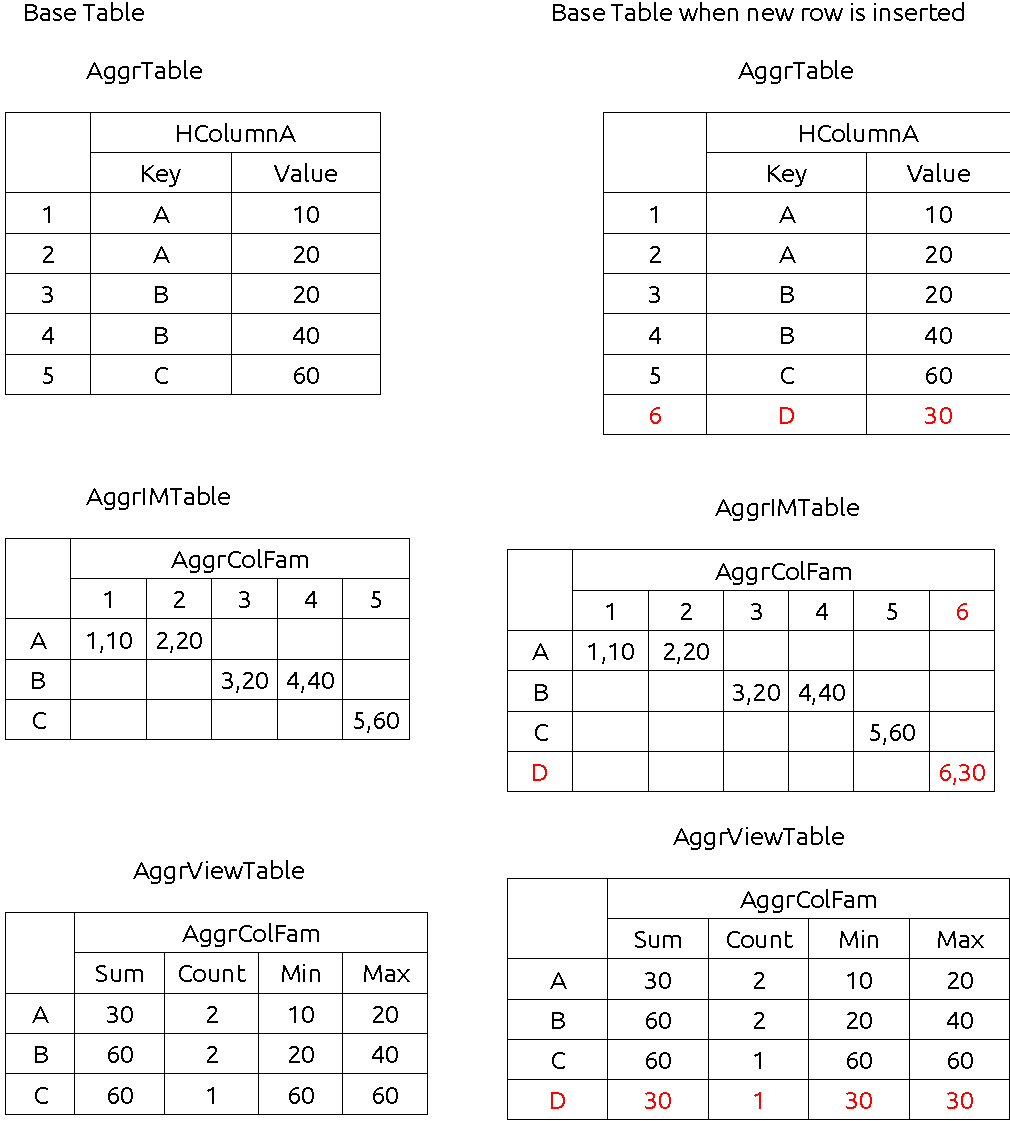
\includegraphics[width=\linewidth]{NewRowInsertAggr}
    \caption{New row insert}
    \label{sec:newrowinsertagggregation}
    
\end{figure}

\newpage
\subsubsection{Existing value of a row is updated}
Whenever an existing value of a key is updated, the base table is updated accordingly. Before the base table is updated, we catch the request via prePut() method of observer coprocessor. In the prePut() method, we get the row key for which the value is going to be updated and also we verify if the value is being updated or the key is being updated. After we verify that value is updated, then we release the request and the value is updated in the base table. After the insertion, we catch the request via postPut() method of observer coprocessor, and then plot the updated value in our intermediate table for particular row key. Since we already have  the row key, we only need to can that particular row, instead of scanning the whole table. This saves a lot of execution time and processing power. Once we plot updated value in the intermediate table, we then calculate aggregation functions for that particular row key and then update our view table accordingly.
The figure below explains the process in more detail. The updated value is marked in red on the right table, and also from the figure, we can see that we only iterate over a particular row key instead of scanning the whole base table and view table.

\begin{figure}
    \centering
    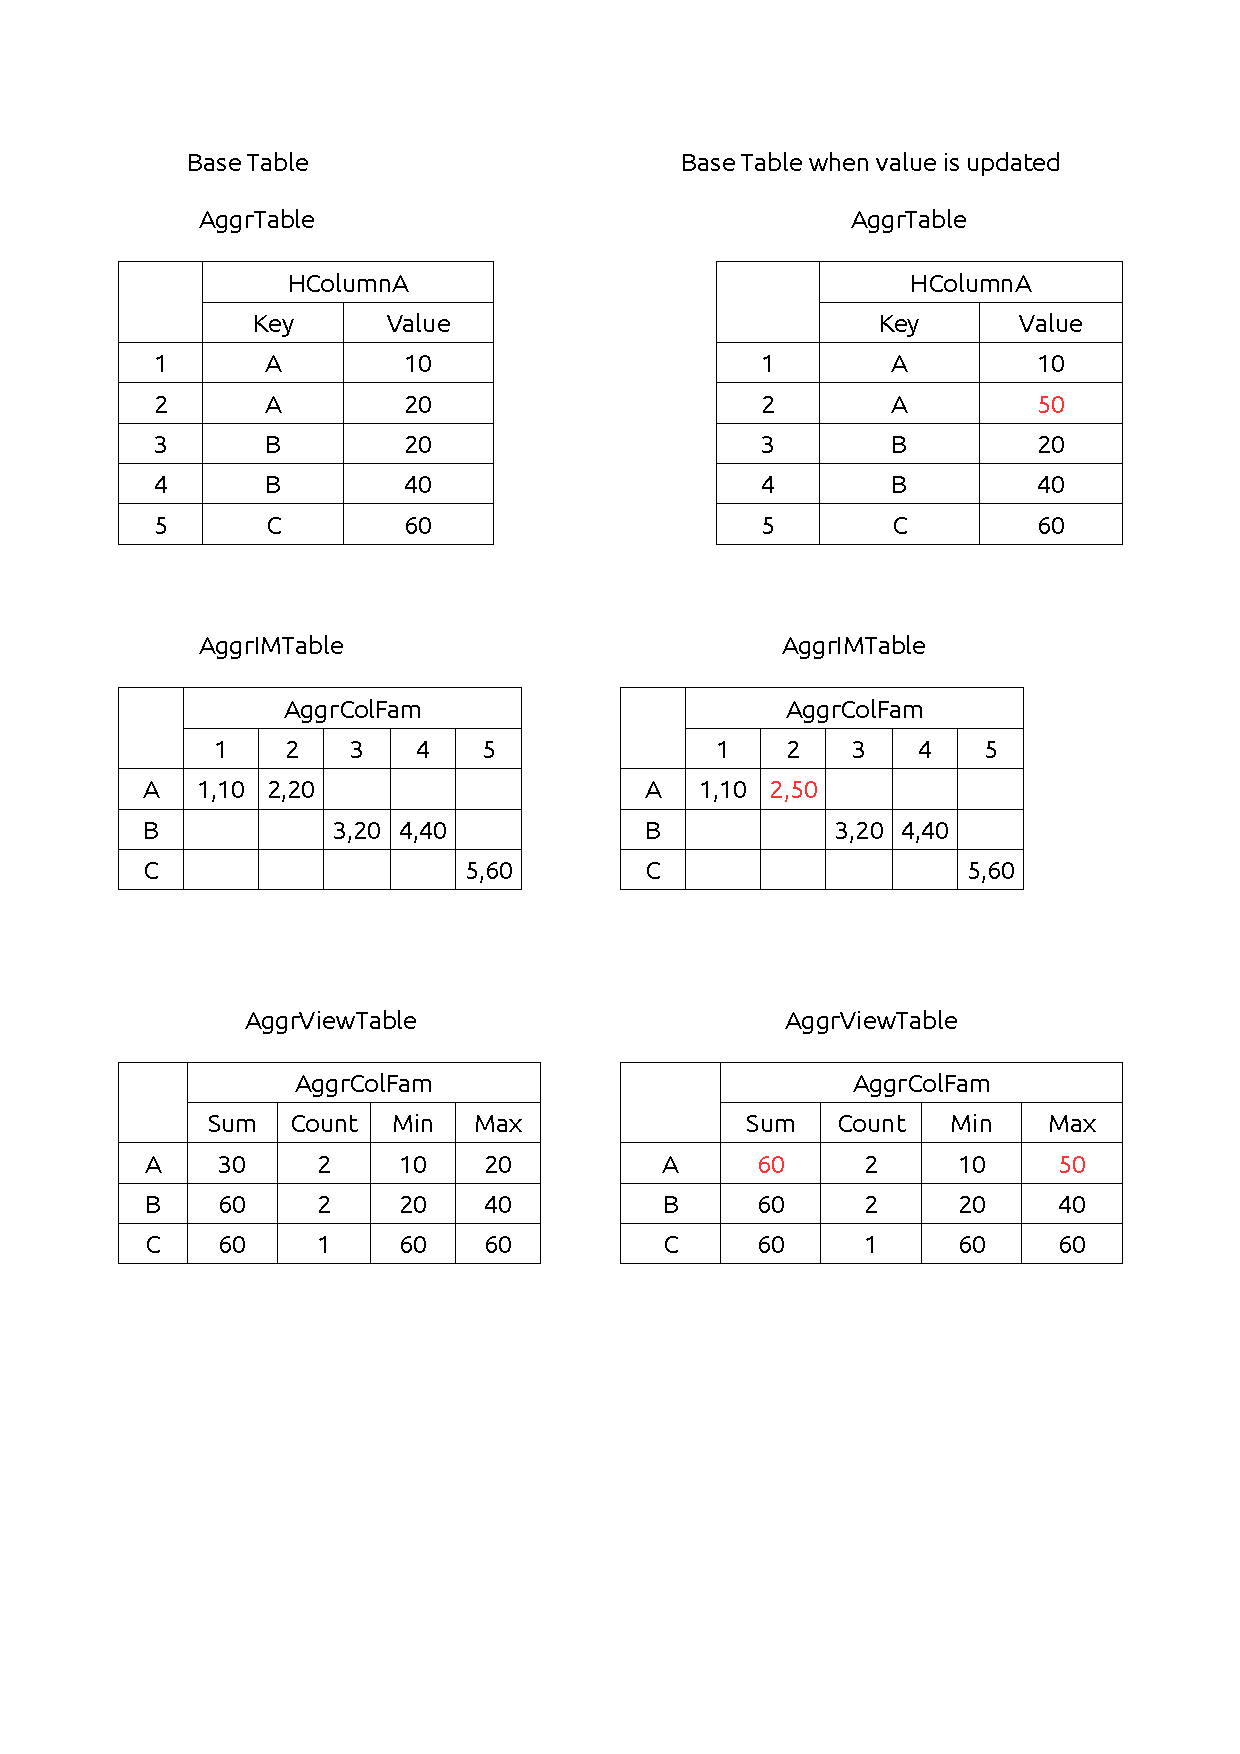
\includegraphics[width=\linewidth]{ValueUpdateAggr}
    \caption{Update value for a existing row key}
    \label{sec:updatevalueforexistingkey}
    
\end{figure}  

\newpage
\subsubsection{Existing key of a row is updated}
\label{subsubsec:keyupdate}
Whenever there is a trigger for $key$ of the particular row key to be updated, we first catch the request via prePut() method. In this scenario, we first have to find out the $key$ to be updated and delete the plotting from intermediate table. In the prePut() method, we find the (key,value) pair for a $key$ to be updated and store it somewhere in memory. Then we release the request and the $key$ is updated in the base table. In this case, now we have $old$ $key$ and the $new$ $key$. 

In the postPut() method, first we find the column to be deleted from the intermediate table. Then we delete that particular column and update our view table accordingly. After the process is complete without any interruption, the process is similar as of inserting new (key,value) pair. We plot the $new$ $key$ and $value$ in our intermediate table and update the view table accordingly. This is the most complex scenario because it might affect more than one row in our view table. In the figure below, the old key $A$ is updated to new key $B$. In the intermediate table, the plotting for old key $A$ is deleted and aggregation functions for old key $A$ are also updated in the view table. After the process is completed, new values for updated key $B$ is plotted in the intermediate table and then the view table for row key $B$ is also updated accordingly.

\begin{figure}
    \centering
    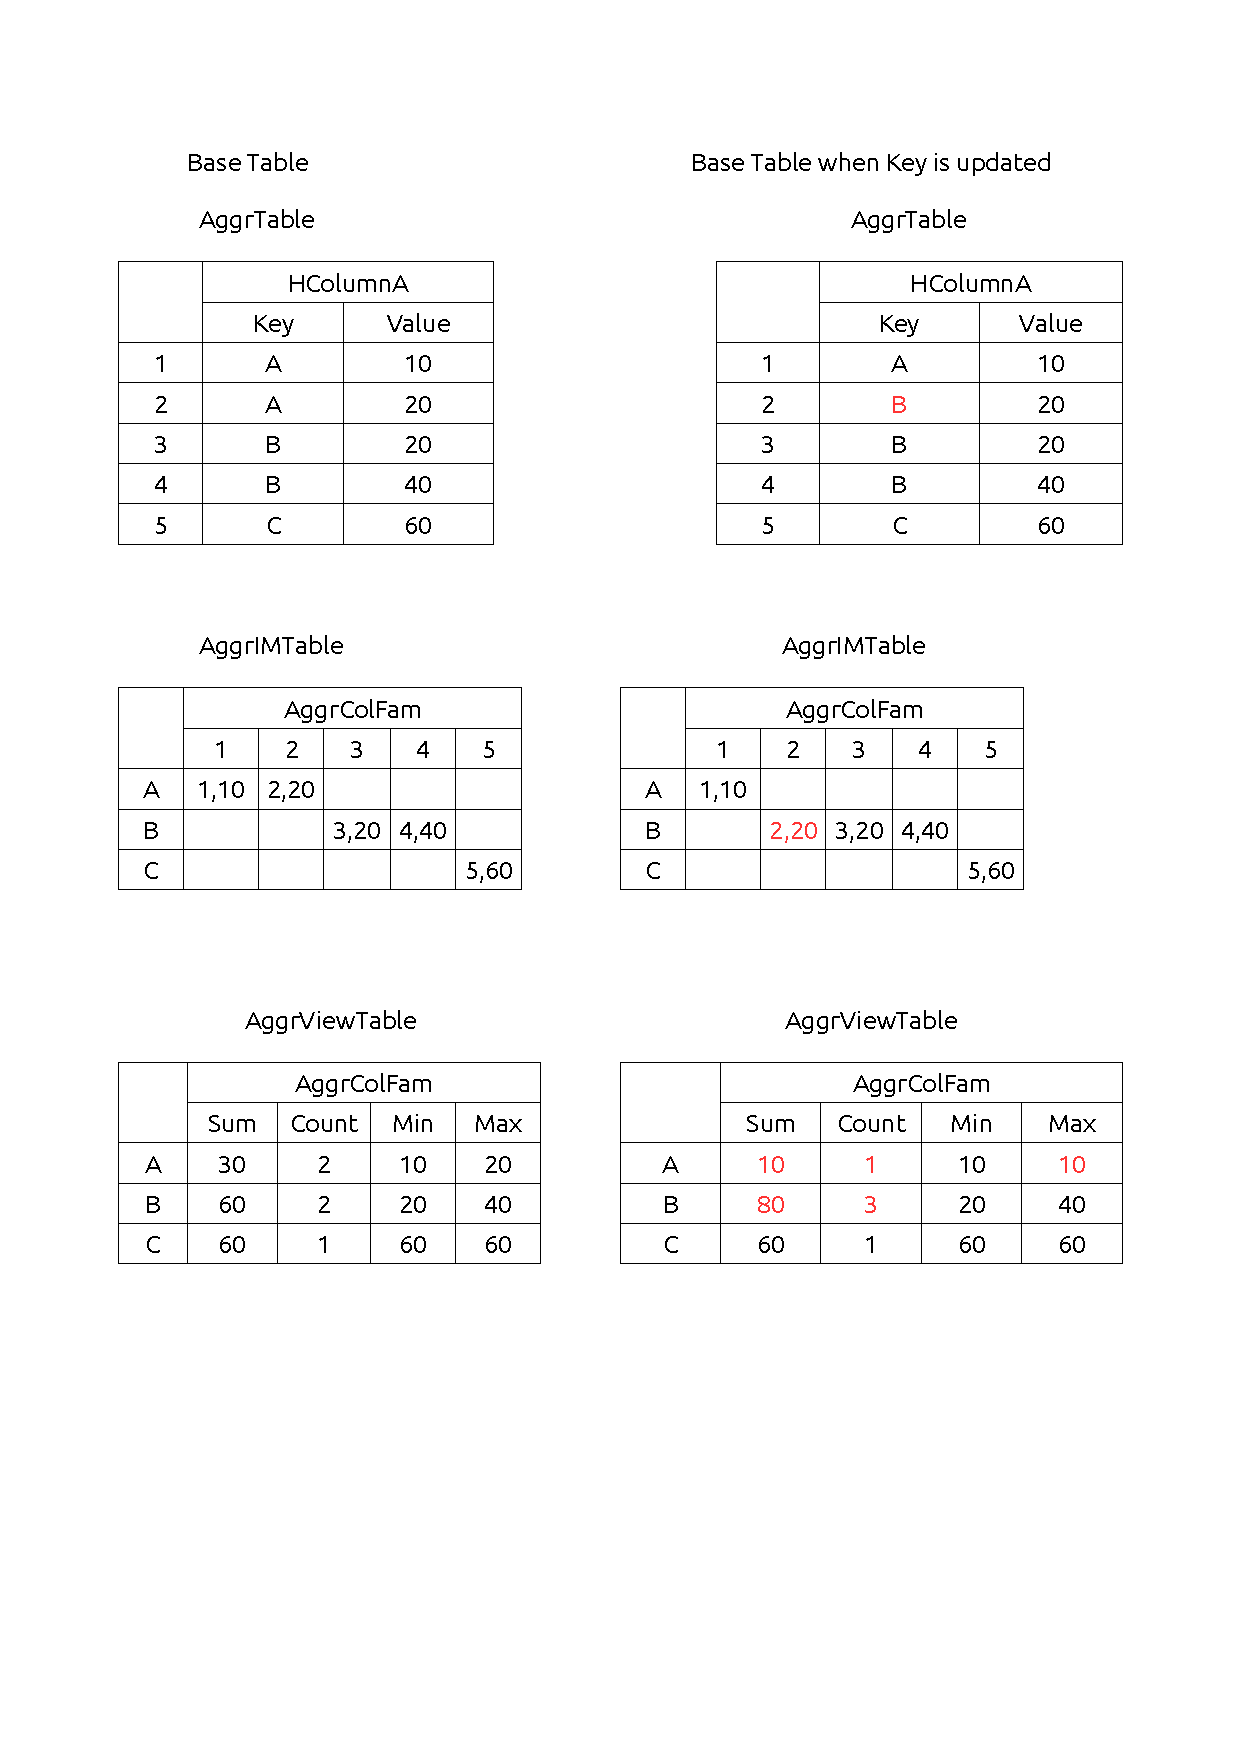
\includegraphics[width=\linewidth]{KeyUpdateAggr}
    \caption{Update Key for a existing row key}
    \label{sec:updateKeyforexistingrow}
    
\end{figure} 

\newpage
\subsubsection{Existing row is deleted}
\label{subsubsec:rowdelete}
When an existing row is deleted in the base table, in the postPut() method of observer coprocessor, we delete the plotting for that particular $key$. In this case, there are two scenarios. If the $key$ to be deleted has more than one values in the intermediate table, then we delete the particular plotting in the intermediate table and update aggregation functions for that $key$ in the view table. If the $Key$ in the intermediate table only has a single plotting, then we delete that plotting from an intermediate table and then also delete the entry for that $key$ from the view table.

In the figure below, we have a delete() call for row key $5$. The $key$ for row key $5$ is $C$. Now we delete the row key $5$ from the base table. After that, we delete the plotting for key $C$ in our intermediate table. Since the key $C$ has only one plotting, we delete entry for row key $C$ from the view table instead of recomputing aggregation functions for row key $C$. 

\begin{figure}
    \centering
    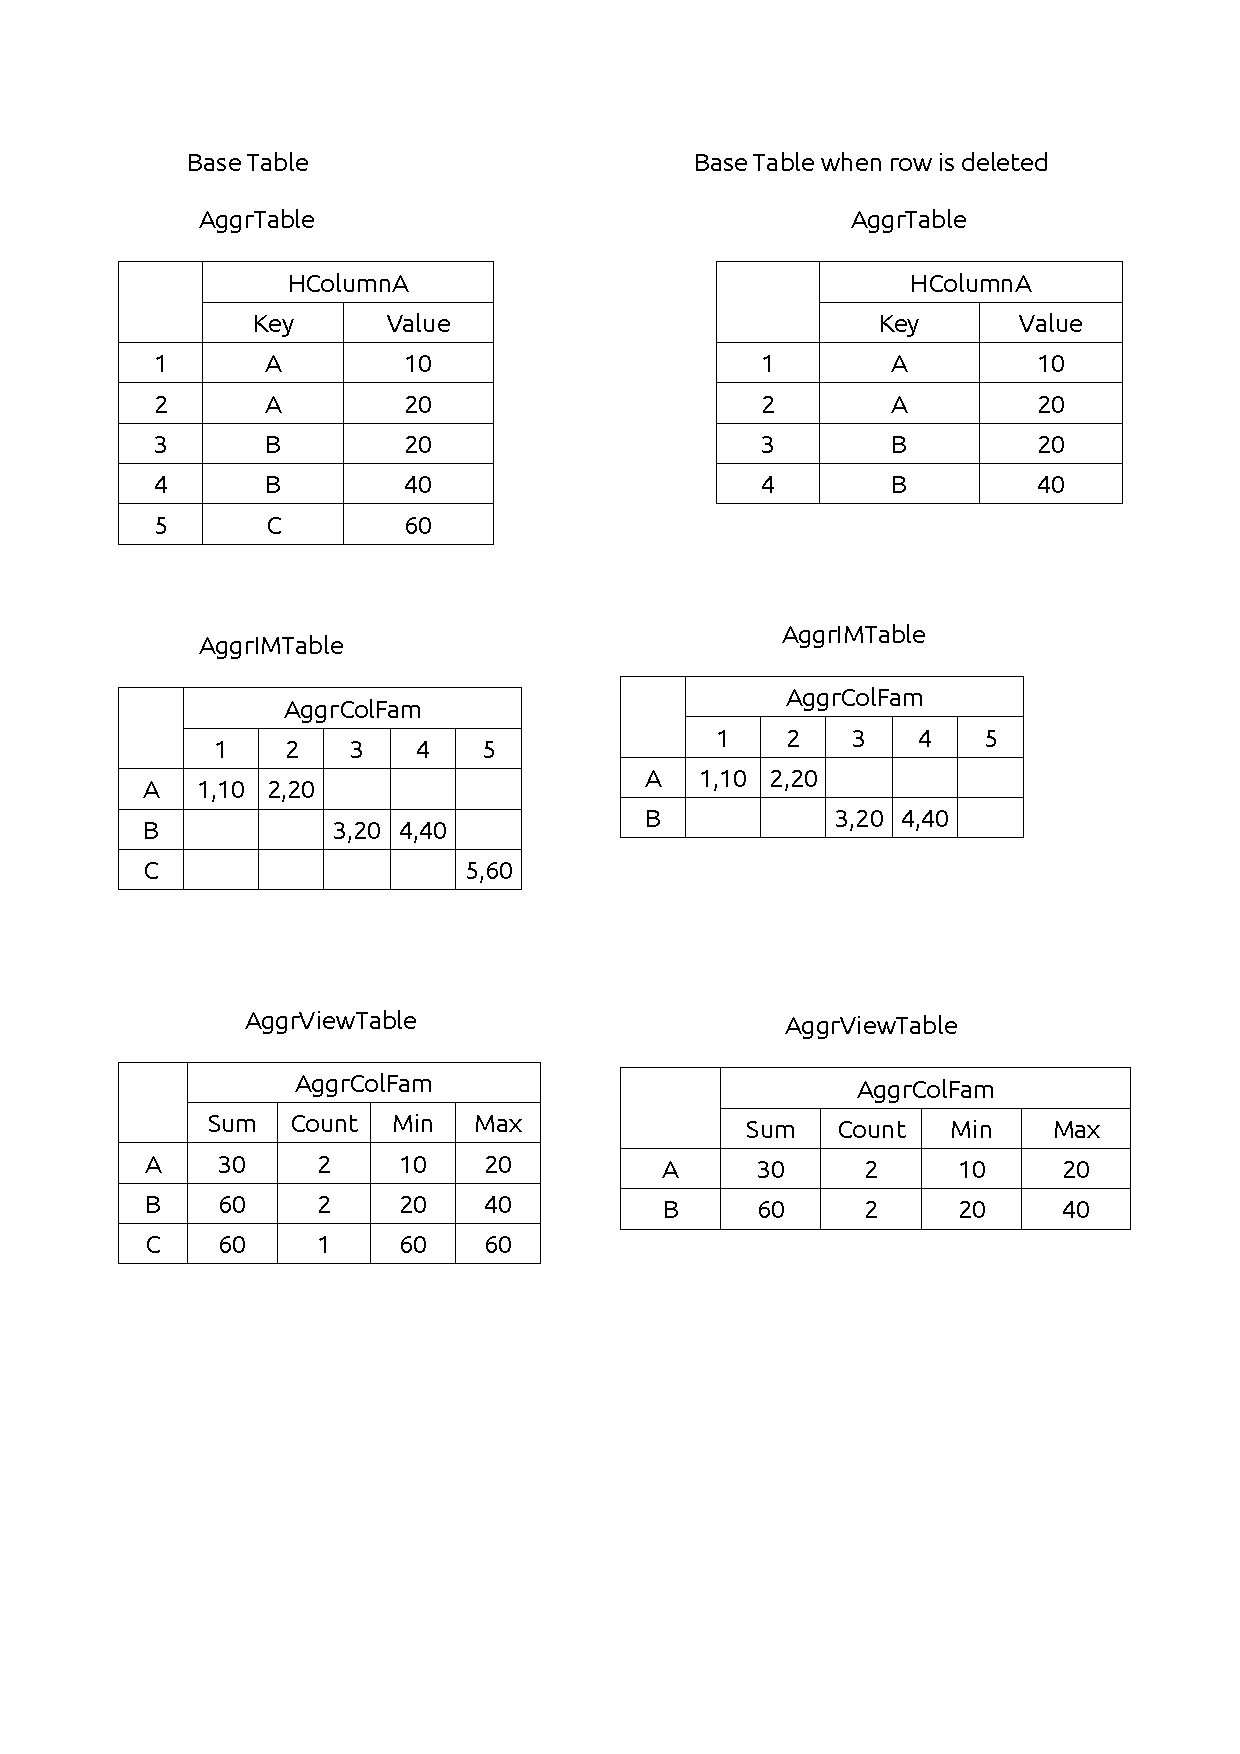
\includegraphics[width=\linewidth]{DeleteExistingRowAggr}
    \caption{Delete an existing row}
    \label{sec:deleteexistingrow}
    
\end{figure} 

\newpage
\subsection{Join and Aggregation}
\label{subsec:joinandaggregation}
In this subsection, we have implemented Join and Aggregation functionalities. For this, we have joined two base tables and in the view table, we have the sum of the values for a same $key$. We also have an intermediate table where both the base tables are merged by a particular $key$ and values are plotted in the intermediate table base on that $key$. As described in \ref{sec:aggregationImpl}, we have implemented sum for same $key$ in both the base tables. 

%The figure below explains how we map base table to a view table.

%\begin{figure}
%    \centering
%    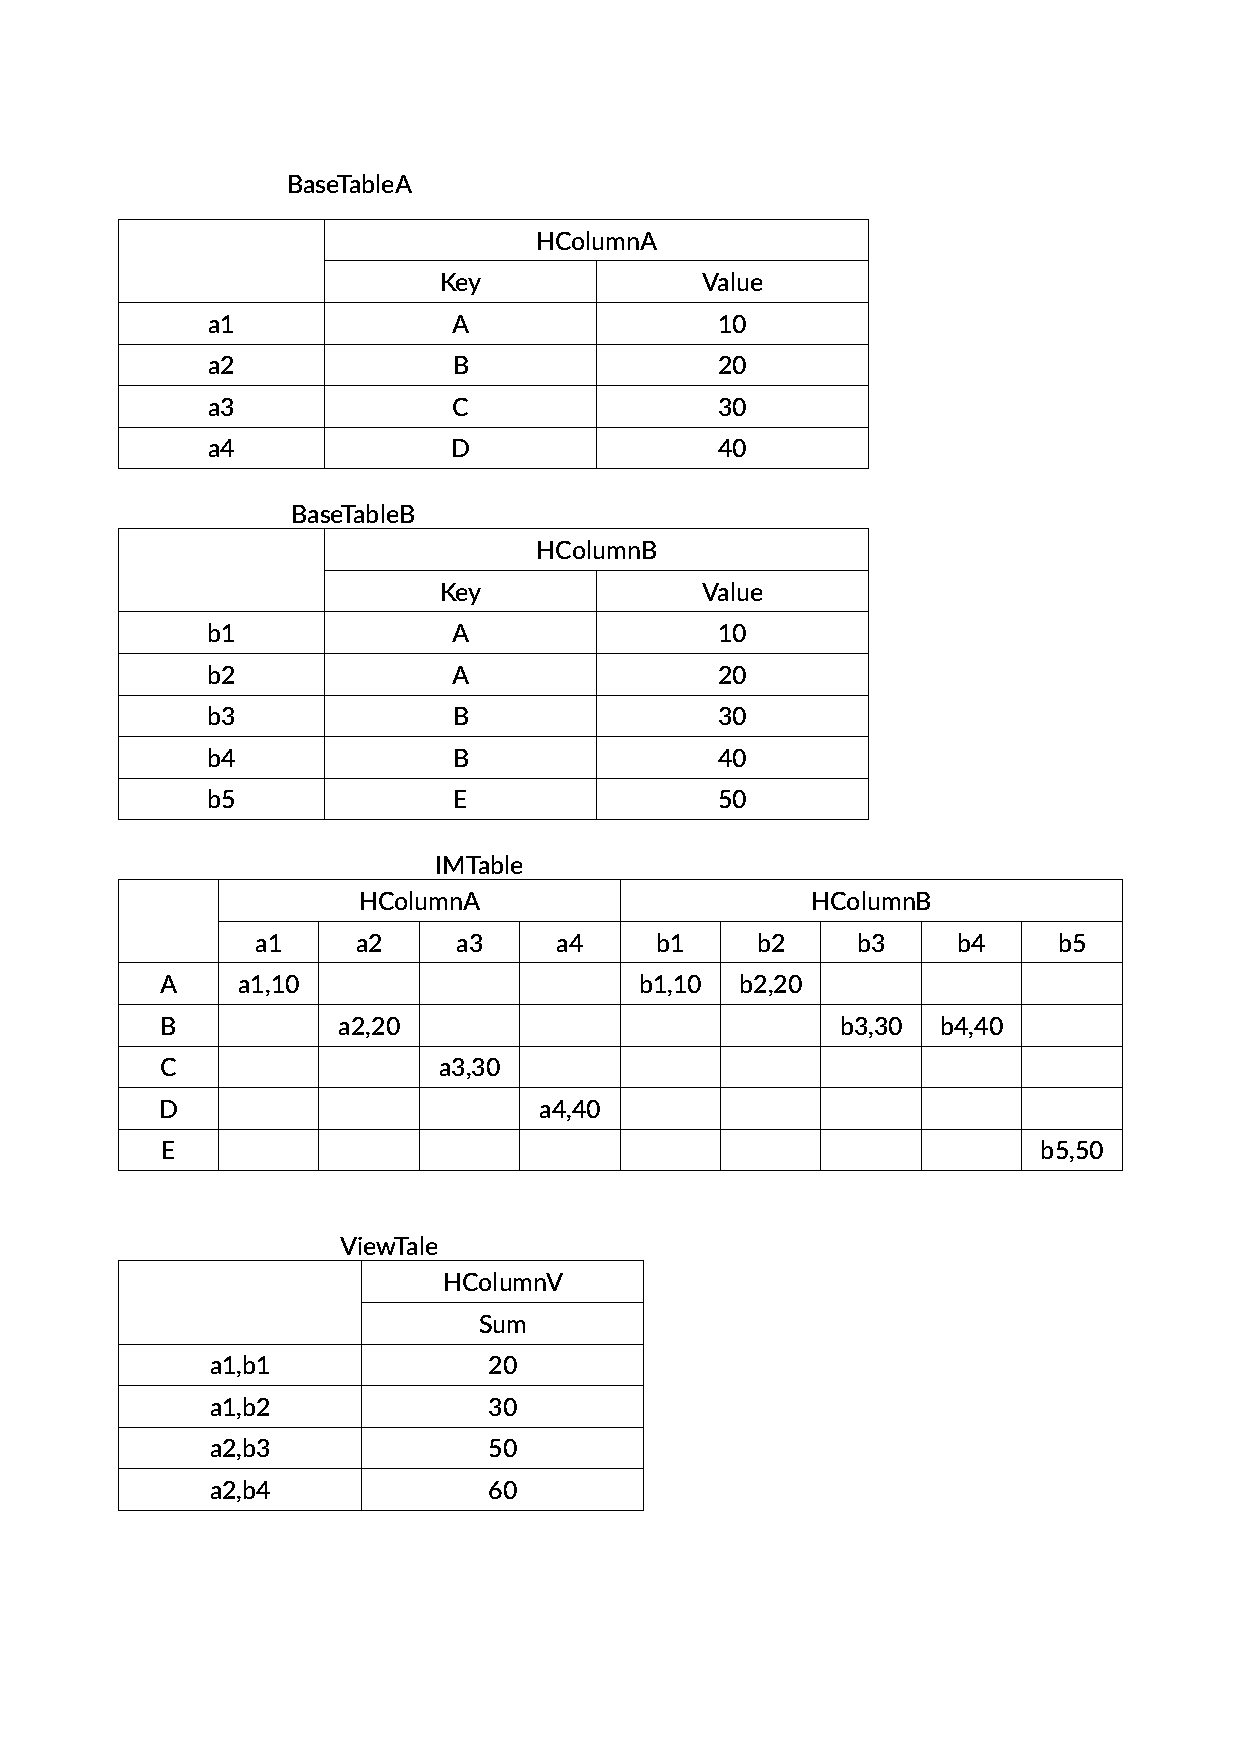
\includegraphics[width=\linewidth]{JoinAndAggregation}
%    \caption{Join and Aggregation}
%    \label{sec:joinandaggregation}
    
%\end{figure}

%\newpage
There are certain scenarios where coprocessor is triggered for an update and delete operations.

\begin{enumerate}
    \item New row is inserted
    \item Existing value of a row is updated
    \item Existing key of a row is updated
    \item Existing row is deleted
\end{enumerate}

\subsubsection{New row is inserted}
Whenever a new row is inserted in a base table with (key,value) pair, the (key,value) pair has to be inserted in the base table and we have to plot the new (key,value) pair in the intermediate table and also view table has to be updated accordingly. Here, we create an intermediate table by merging two base tables and plotting values accordingly. The algorithm for plotting values has already been discussed in sub section \ref{subsec:intermediatetable}. In the view table, we implement sum function for same $keys$ in both base tables.
The figure below describes the scenario in more detail. The updated table on the right has new values plotted in red.

\begin{figure}
    \centering
    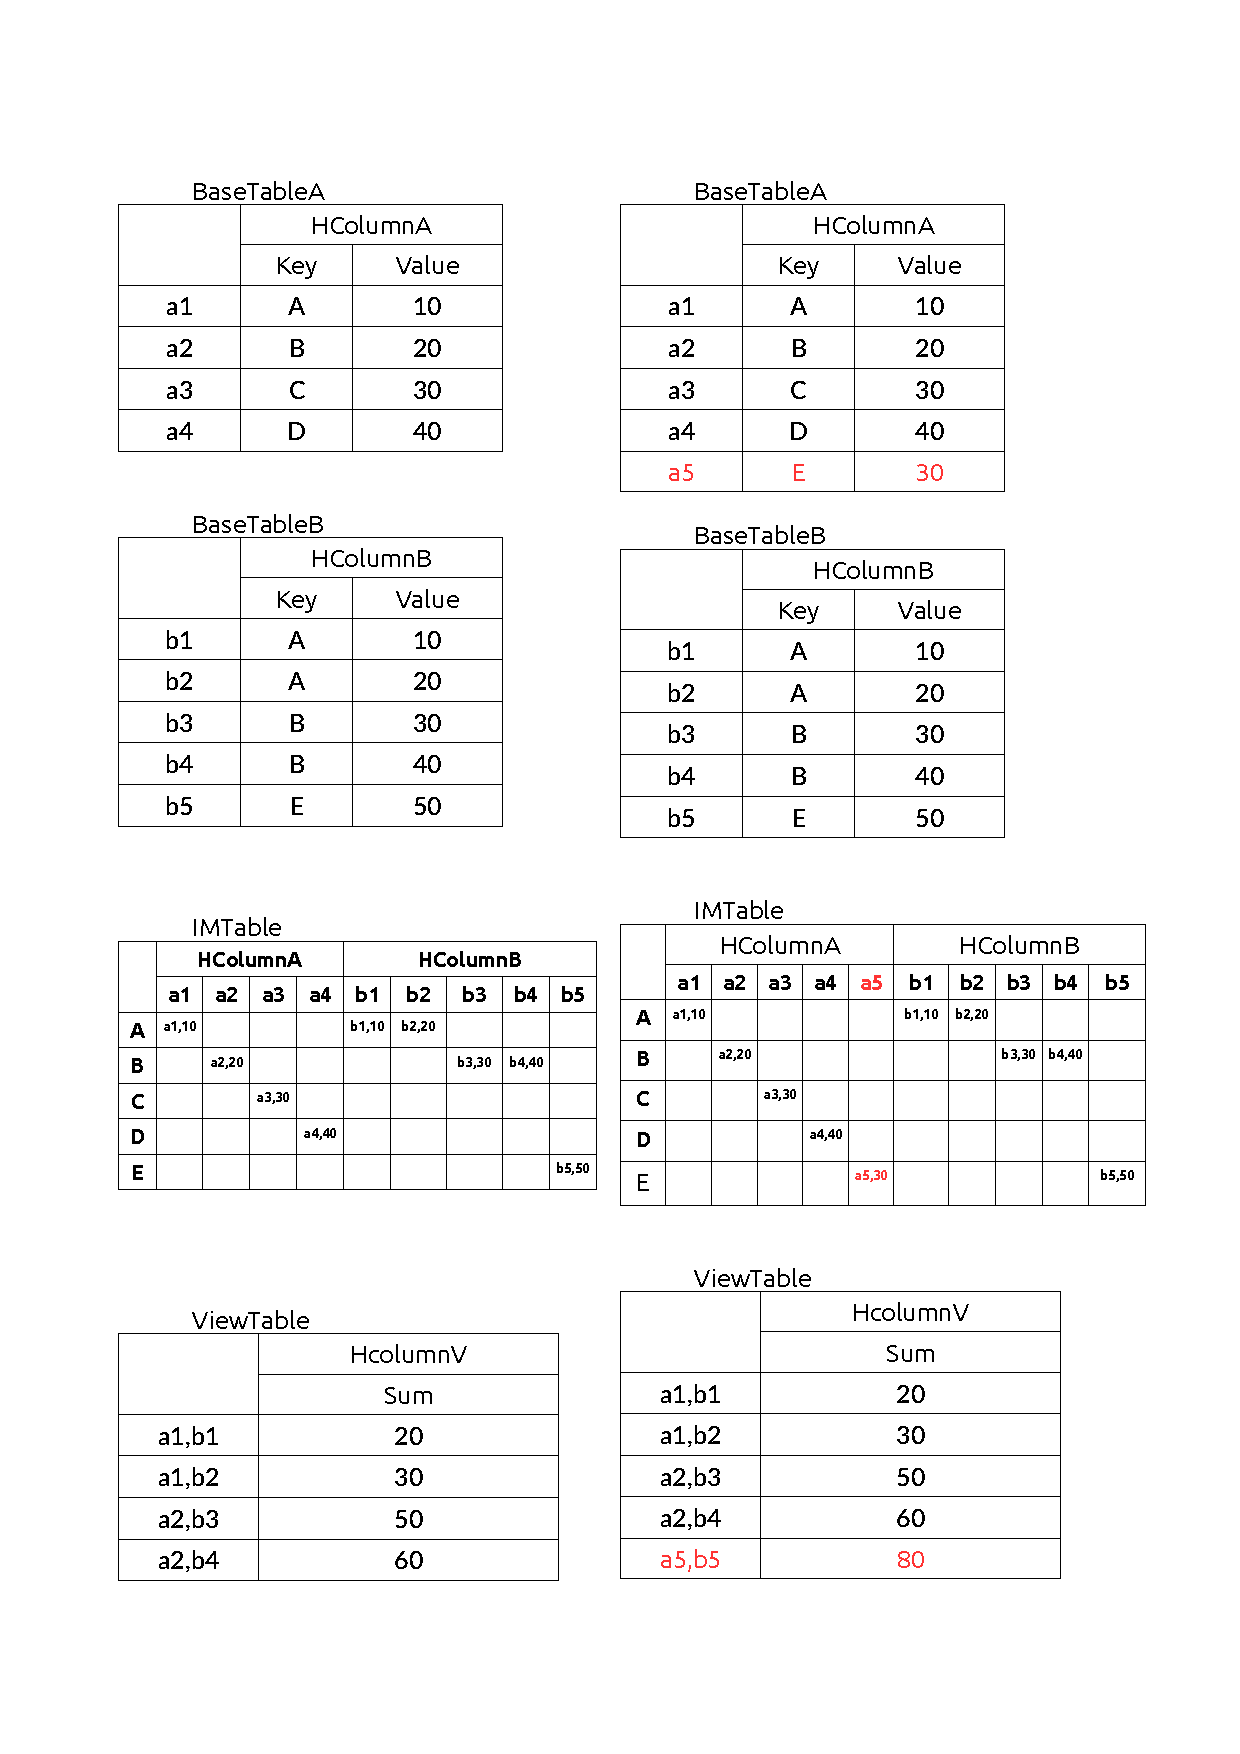
\includegraphics[width=\linewidth]{NewRowInsertJoinAggr}
    \caption{New row is inserted for Join and Aggregation}
    \label{sec:insertnewrowjoinandaggr}
    
\end{figure}

\newpage

\subsubsection{Existing value of a row is updated}
When a value of a $key$ is updated in the base table, the consistency should also be maintained in the view table. So when the base table is updated, the request is triggered by the postPut() method and intermediate table and view tables are updated accordingly.

\subsubsection{Existing key of a row is updated}
As described in \ref{subsubsec:keyupdate}, when $key$ is modified in the base table, we first have to delete an entry from the intermediate table and view table if the row exists for that particular $key$. Once delete operation is completed without interruption, then we insert the updated key in the intermediate table and view table.

\subsubsection{Existing row is deleted}
The implementation for this scenario is same as described in subsection \ref{subsubsec:rowdelete}. The entry is first deleted from the base table, and if an entry exists in the intermediate table and view table, the entries are deleted from those table accordingly.

\subsection{Join and Selection}
This approach is similar to approach described in subsection \ref{subsec:joinandaggregation}. We do not use any aggregation functions but instead just select the values and put them in the view table. As already described in \ref{subsec:joinandaggregation}, there are also four possible scenarios where we update view table incrementally.

\newpage
\chapter{Discussion and Conclusion}


		% ---------------------------------------------------------------------------
		%
		% Appendix
		%
		% ---------------------------------------------------------------------------
		
		\part*{Appendix}
		\addcontentsline{toc}{part}{Appendix}
		
		\appendix %---------------------------------------
		
		%\chapter{Components}
%\section{Detailed Validation Results}
\label{chapter:Components}

\section{VM Master}


\textbf{Interface}

\begin{enumerate}
	\item Ingoing
	\begin{itemize}
		\item $viewManagerAdded$
		\item $viewManagerAssigned$
		\item $viewManagerRemoved$
		\item $viewManagerWithdrawn$
		\item $viewManagerReassigned$
		\item $regionServerAdded$
		\item $regionServerRemoved$
		\item $callLastCommitedUpdate$
	\end{itemize}
	\item Outgoing
	\begin{itemize}
		\item $createZookeperNode$
		\item $assignViewManager$
		\item $reassignViewManager$
		\item $withdrawViewManager$
		\item $removeViewManager$
		\item $replayWriteAheadLog$

	\end{itemize}
\end{enumerate}


\textbf{Subcomponents}

\begin{enumerate}
	\item $VM\:Master\:Controller$
	\item $Event\:Processor$
	\item $Load\:Balancer$
	\item $Recover\:Manager$
	\item $Component\:Controller$
\end{enumerate}
\newpage
\begin{figure}[h!] 
  \centering
    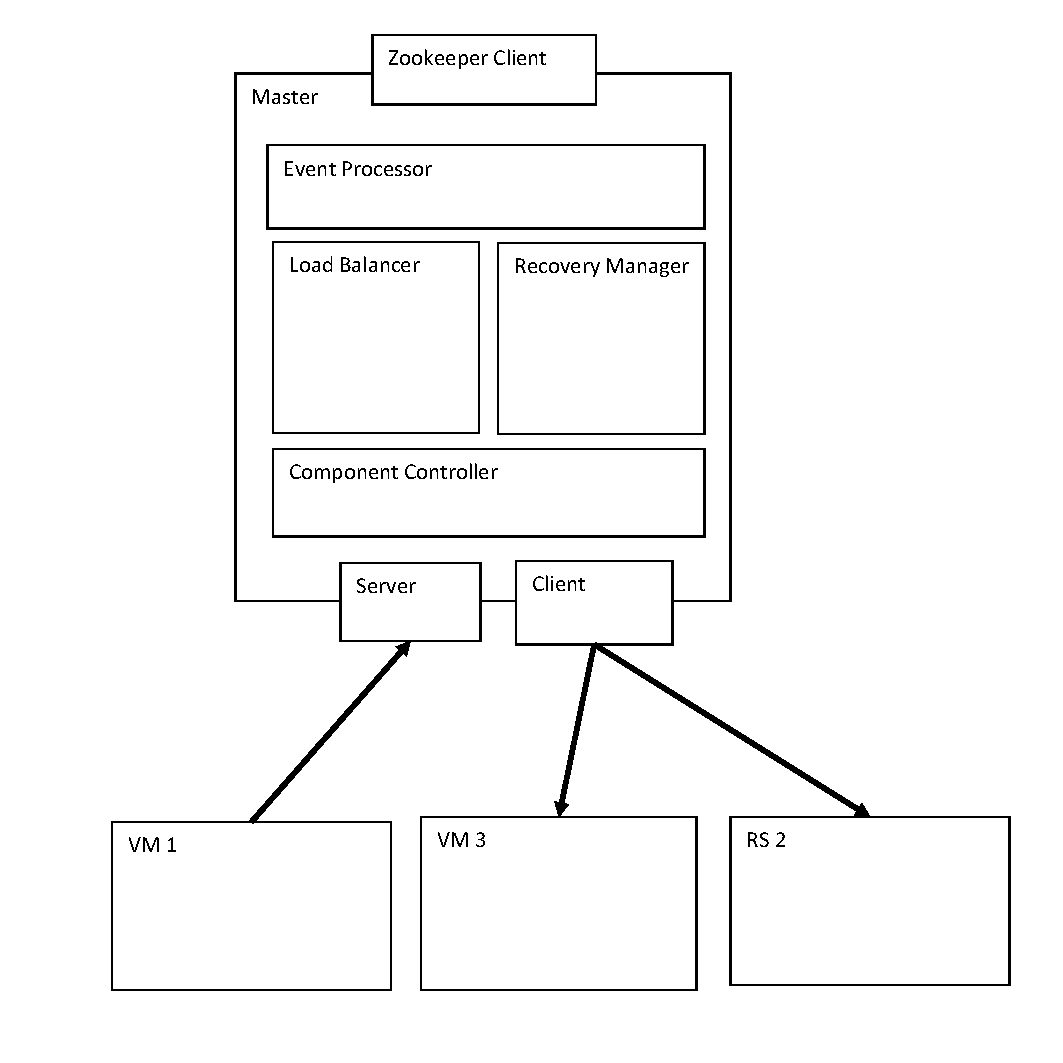
\includegraphics[scale=0.8]{figures/Master}
    \caption{Master}
    \label{fig:master}
\end{figure}

\newpage

\section{VM Region Server}

\textbf{Interface}

\begin{enumerate}
	\item Ingoing
	\begin{itemize}
		\item $put, get, delete$
		\item $assignViewManager$
		\item $withdrawViewManager$
		\item $replayWriteAheadLog$
		\item $statusReportViewManager$
	\end{itemize}
	\item Outgoing
	\begin{itemize}
		\item $createZookeeperNode$
		\item $sendUpdate$
		\item $sendStatusReport$
	\end{itemize}
\end{enumerate}


\textbf{Subcomponents}

\begin{enumerate}
	\item $HBase\:Region\:Server$
	\item $RS\:Controller$
	\item $Write\:Ahead\:Log$
	\item $WAL\:Reader$
	\item $Update\:Assigner$
	\item $Update\:Distributor$
\end{enumerate}

\newpage
\begin{figure}[h!]
  
  \centering
    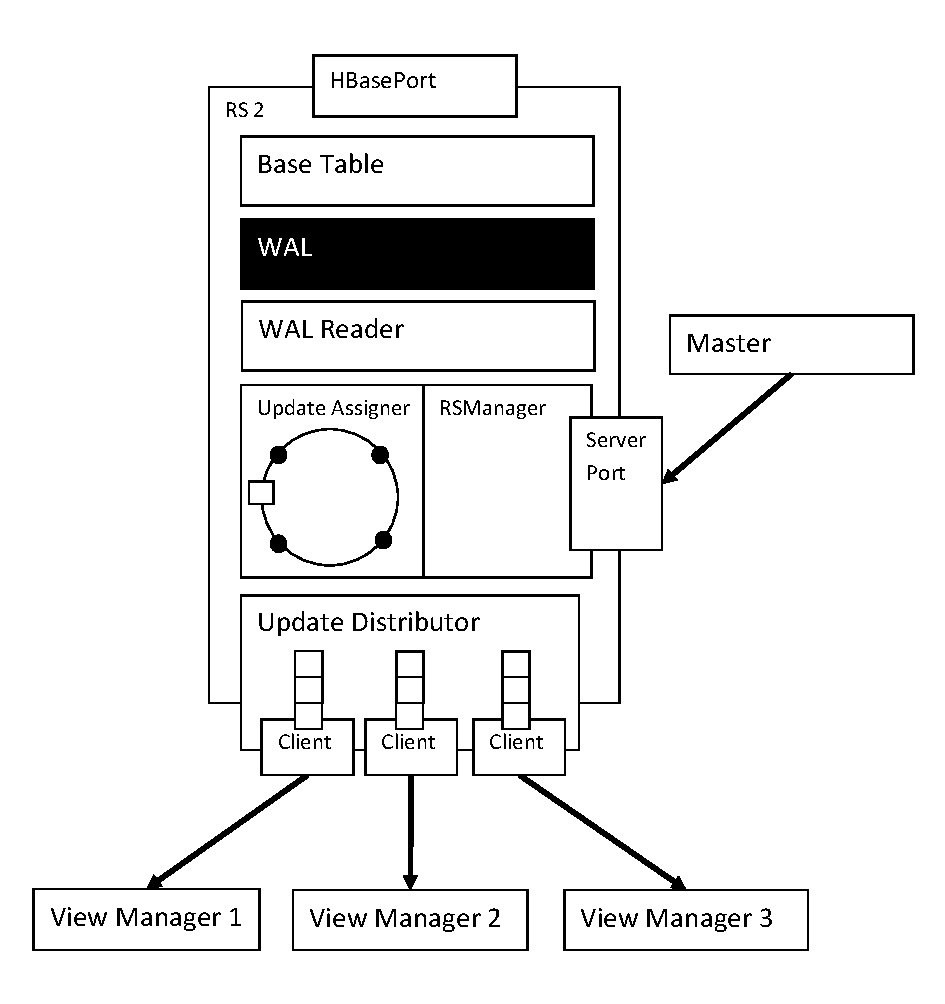
\includegraphics[scale=0.8]{figures/RegionServer}
    \caption{Region Server}
    \label{fig:regionserverAppendix}
\end{figure}
\newpage

\section{View Manager}



\textbf{Interface}

\begin{enumerate}
	\item Ingoing
	\begin{itemize}
		\item $receiveUpdate$
		\item $assignViewManager$
		\item $withdrawViewManager$
		\item $reassignViewManager$
		\item $removeViewManager$
		\item $callLastCommitedUpdate$
	\end{itemize}
	\item Outgoing
	\begin{itemize}
		\item $createZookeeperNode$
		\item $shutdownViewManager$
		\item $assignViewManager$
		\item $withdrawViewManager$
		\item $getViewDefinitions$
		\item $sendStatusReport$

	\end{itemize}
\end{enumerate}

\textbf{Subcomponents}

\begin{enumerate}
	\item $VM\:Controller$
	\item $Pre-Processor$
	\item $Processor$
	\item $Commit\:Log$
\end{enumerate}

\newpage

\begin{figure}[h!]
  
  \centering
    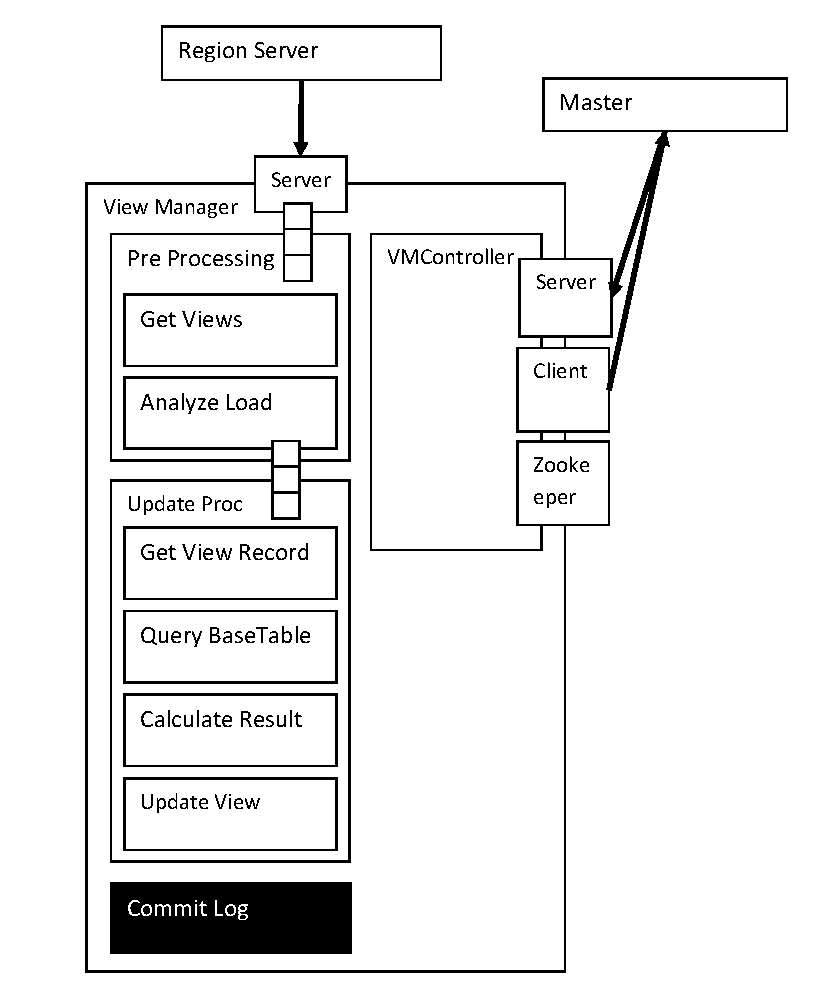
\includegraphics[width=\linewidth]{figures/ViewManager}
    \caption{View Manager}
    \label{fig:viewmanager}
\end{figure}
\newpage



\chapter{System Operations}
\label{chapter:Sytem Operations}


\section{Add View Manager}
\begin{figure}[h!]
  \centering
    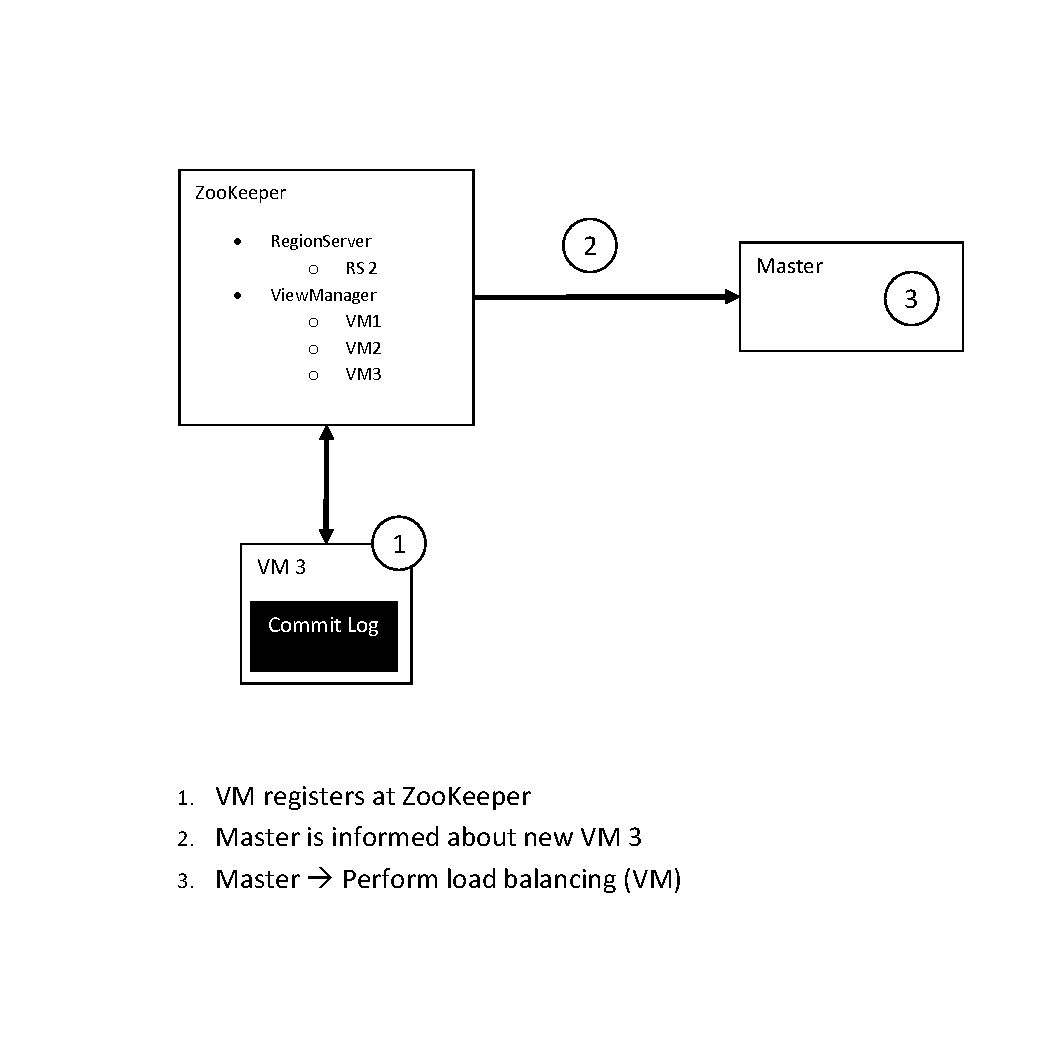
\includegraphics[scale=0.8]{figures/SO_AddViewManager}
    \caption{Add View Manager}
    \label{fig:addviewmanager}
\end{figure}
\newpage

\section{Assign View Manager}
\begin{figure}[h!]
  \centering
    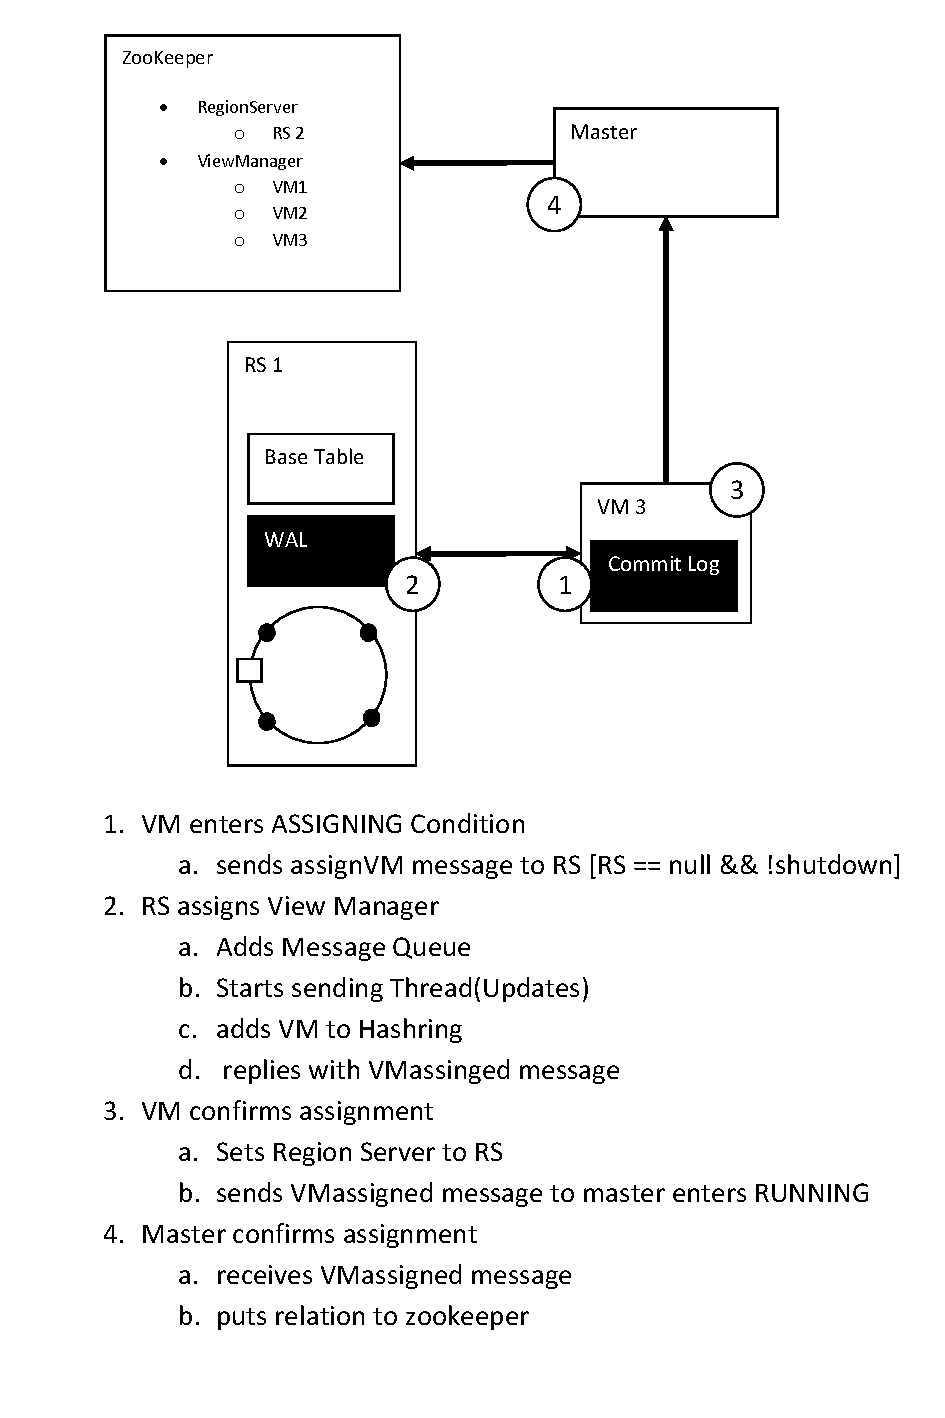
\includegraphics[scale=0.8]{figures/SO_AssignViewManager}
     \caption{Assign View Manager}
    \label{fig:assignviewmanager}
\end{figure}
\newpage

\section{Withdraw View Manager}
\begin{figure}[h!]
  \centering
    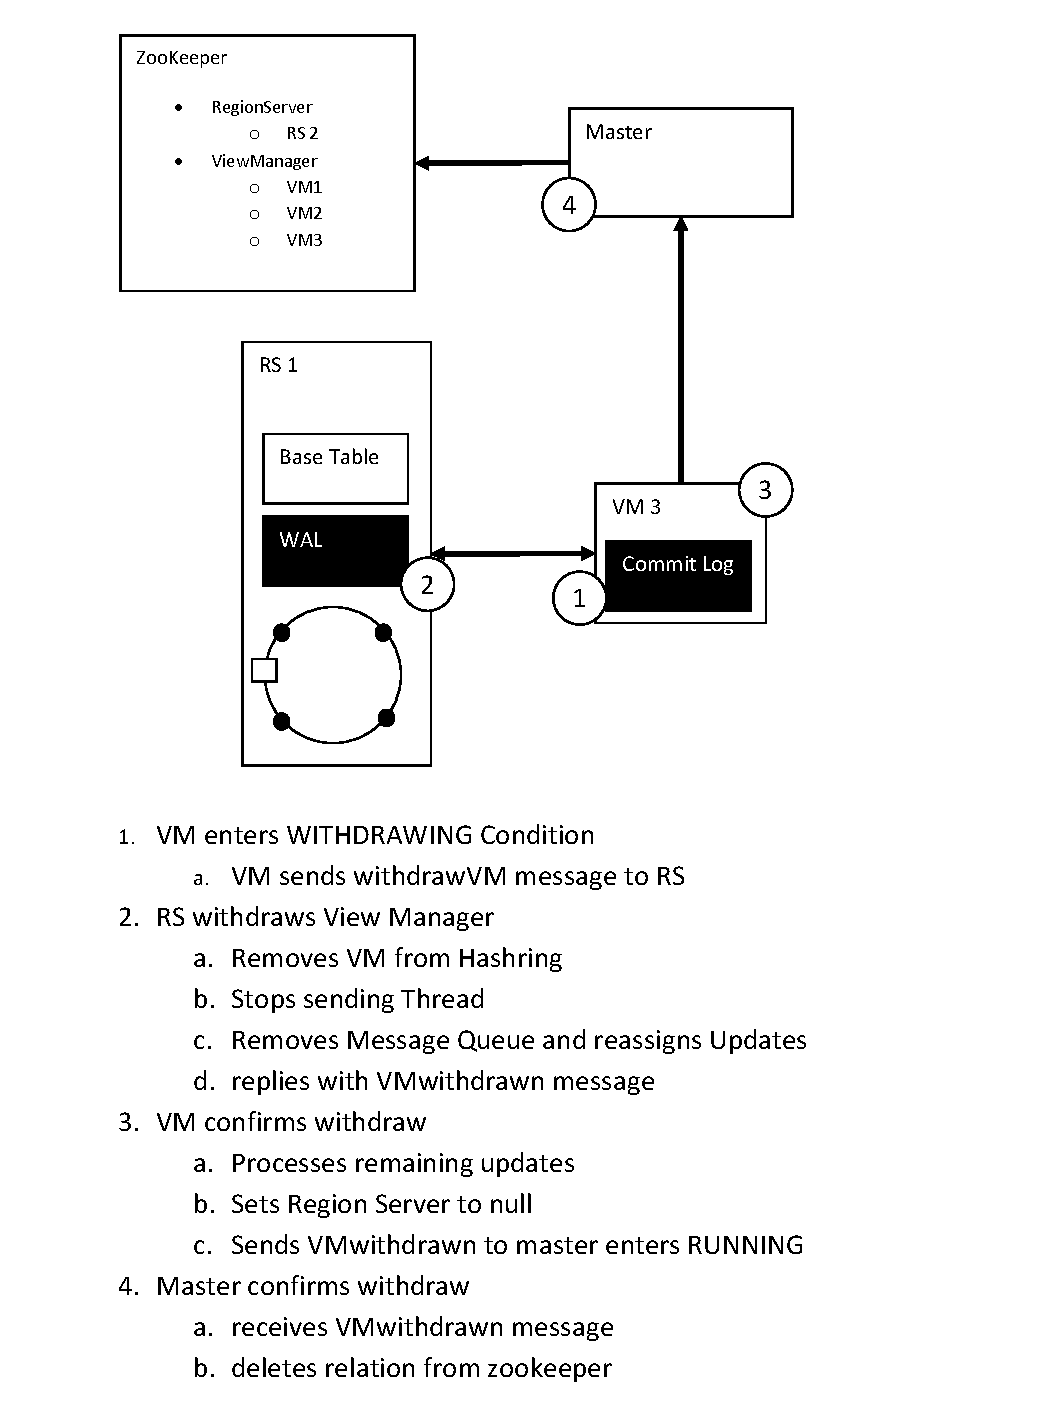
\includegraphics[scale=0.8]{figures/SO_WithdrawViewManager}
     \caption{Withdraw View Manager}
    \label{fig:withdrawviewmanager}
\end{figure}
\newpage
\section{Reassign View Manager}
\begin{figure}[h!]
  \centering
    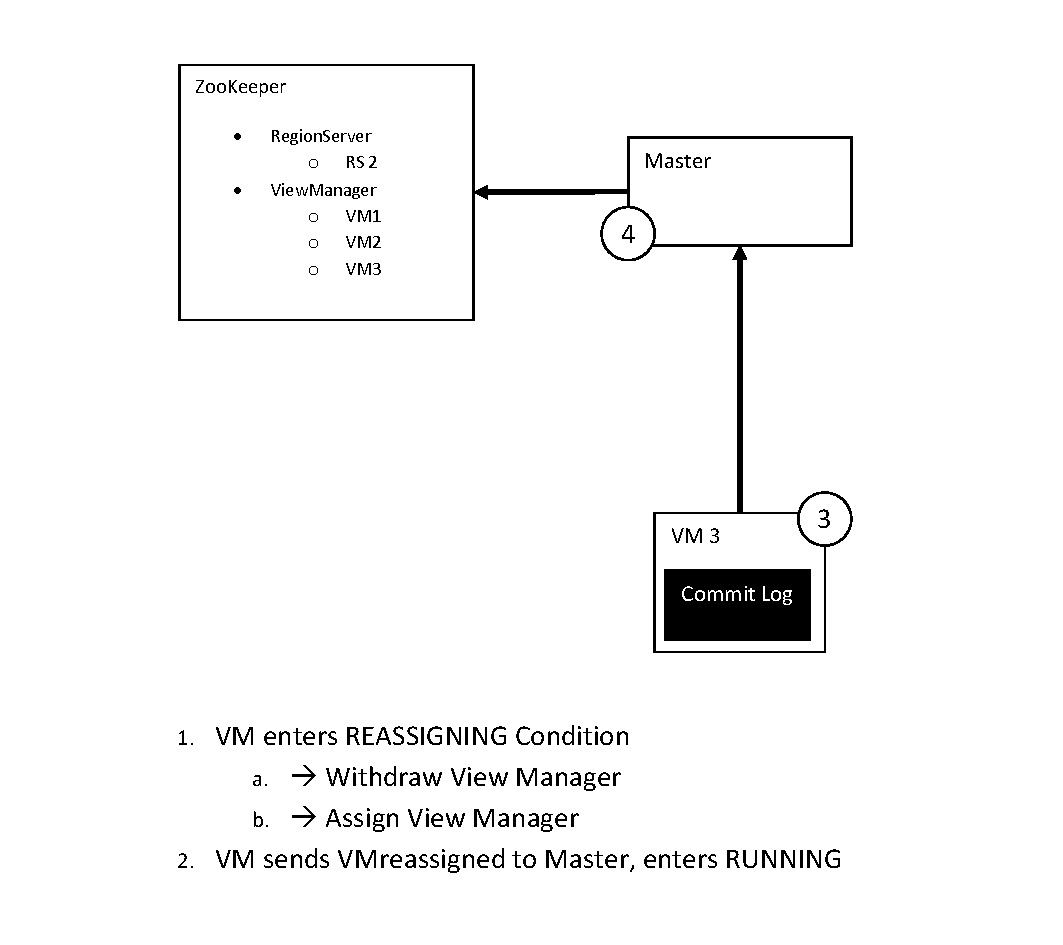
\includegraphics[scale=0.8]{figures/SO_ReassignViewManager}
     \caption{Reassign View Manager}
    \label{fig:reassignviewmanager}
\end{figure}

\newpage

\section{View Manager Crash}
\begin{figure}[h!]
  \centering
    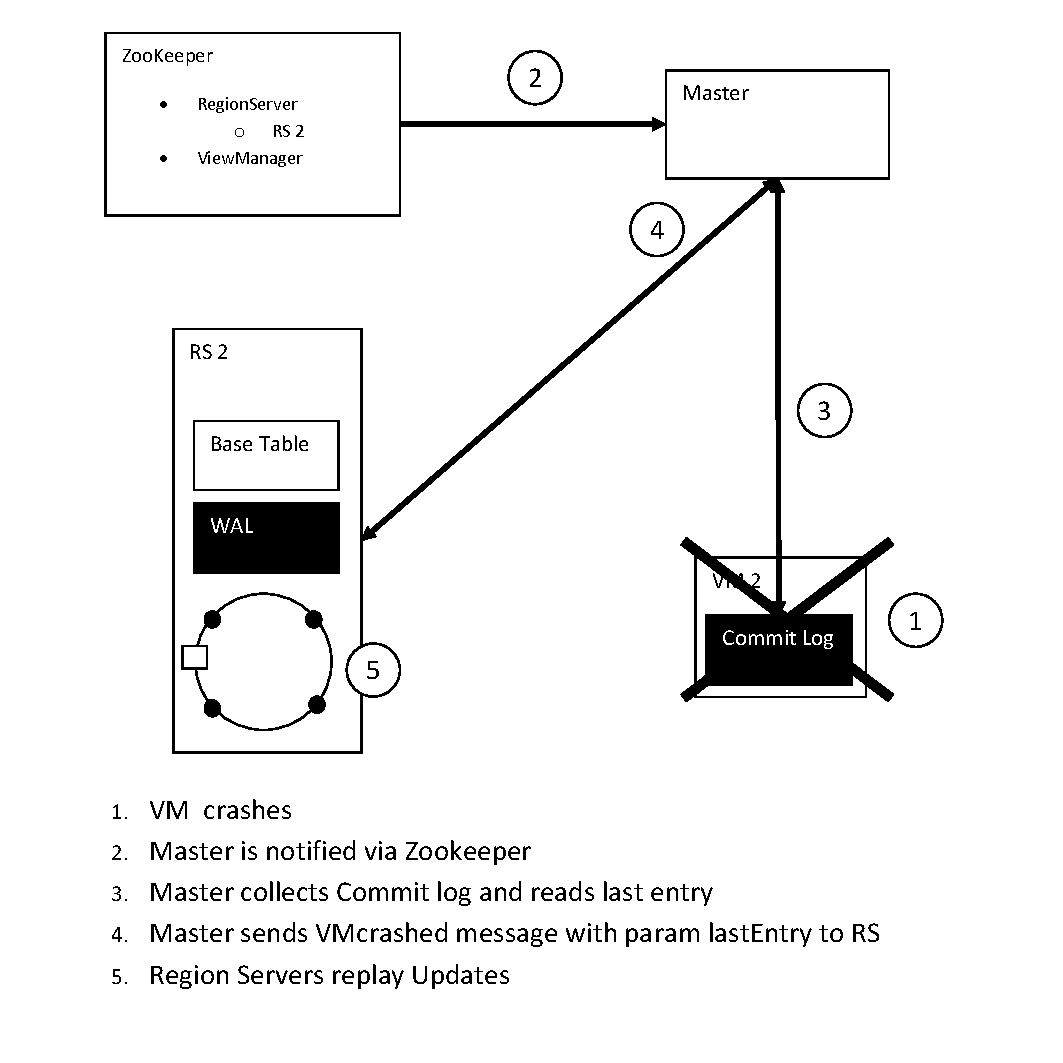
\includegraphics[scale=0.8]{figures/SO_ViewManagerCrash}
     \caption{View Manager Crash}
    \label{fig:so_viewmanagercrash}
\end{figure}
\newpage

\section{Add Region Server}
\begin{figure}[h!]
  \centering
    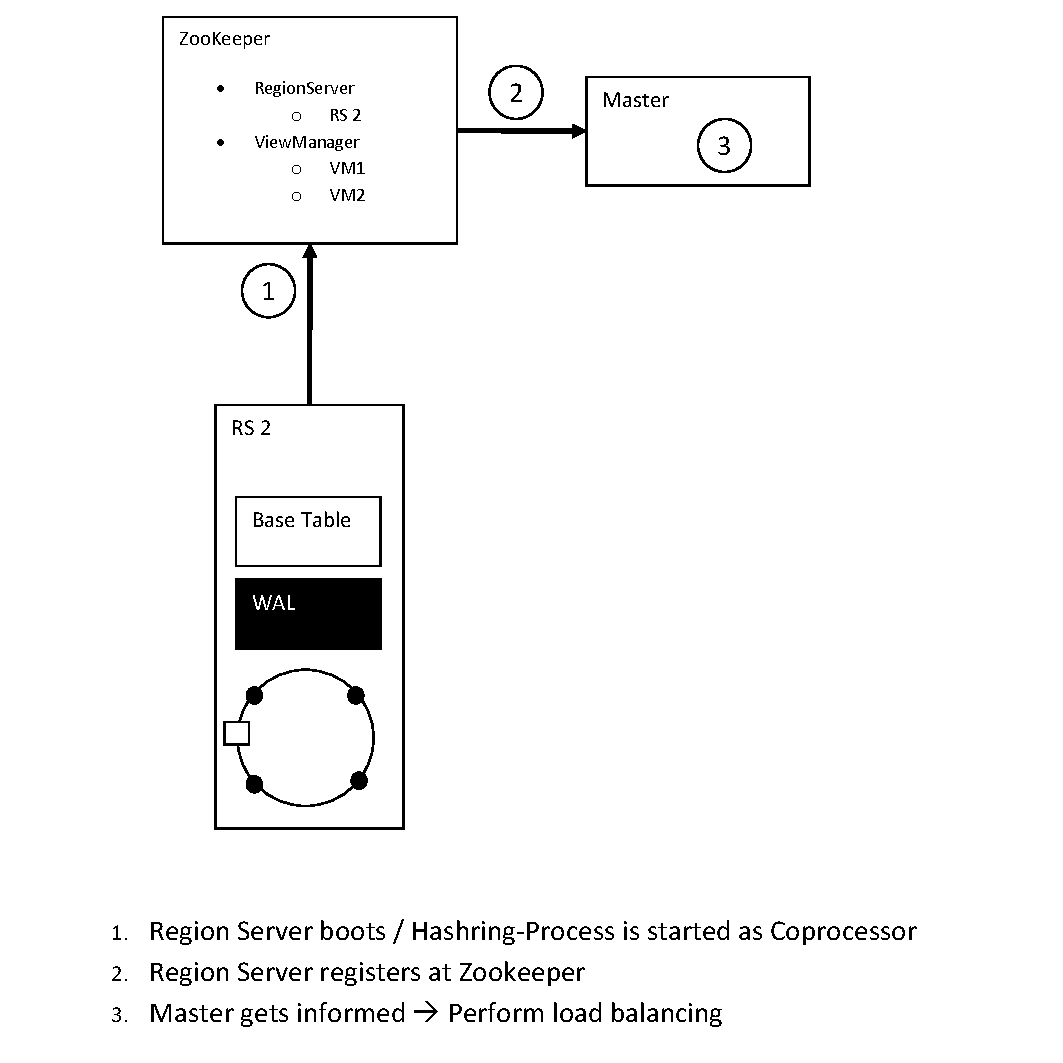
\includegraphics[scale=0.8]{figures/SO_AddRegionServer}
     \caption{Add Region Server}
    \label{fig:addregionserver}
\end{figure}
\newpage

\section{Region Server Crash}
\begin{figure}[h!]
  \centering
    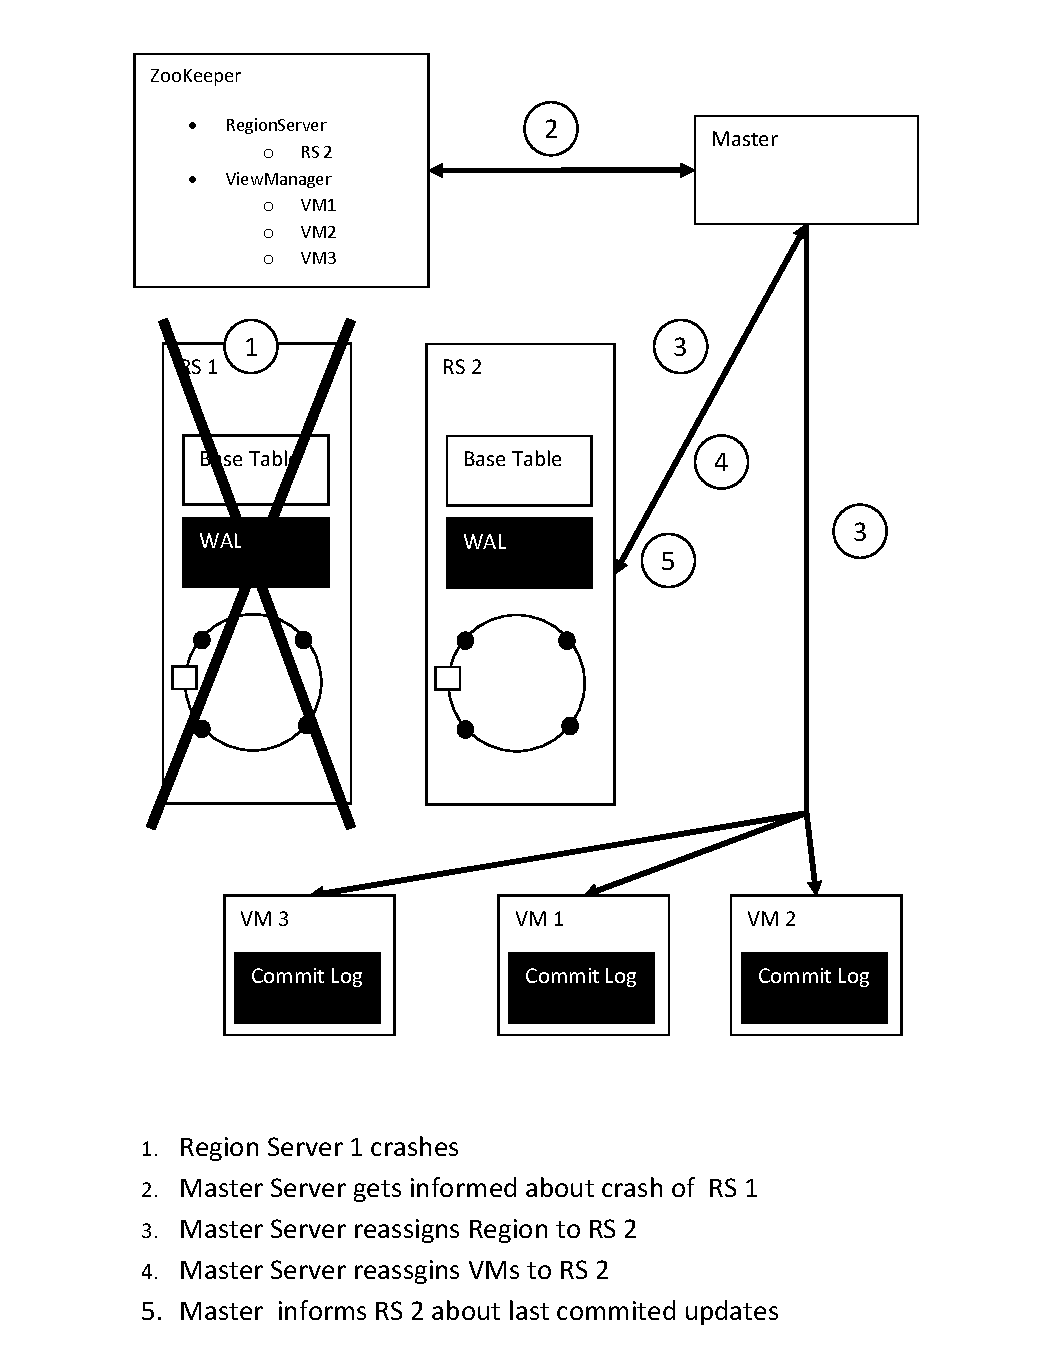
\includegraphics[scale=0.8]{figures/SO_RegionServerCrash}
     \caption{Region Server Crash}
    \label{fig:regionservercrash}
\end{figure}
\newpage

\section{Update Processing}
\begin{figure}[h!]
  
  \centering
    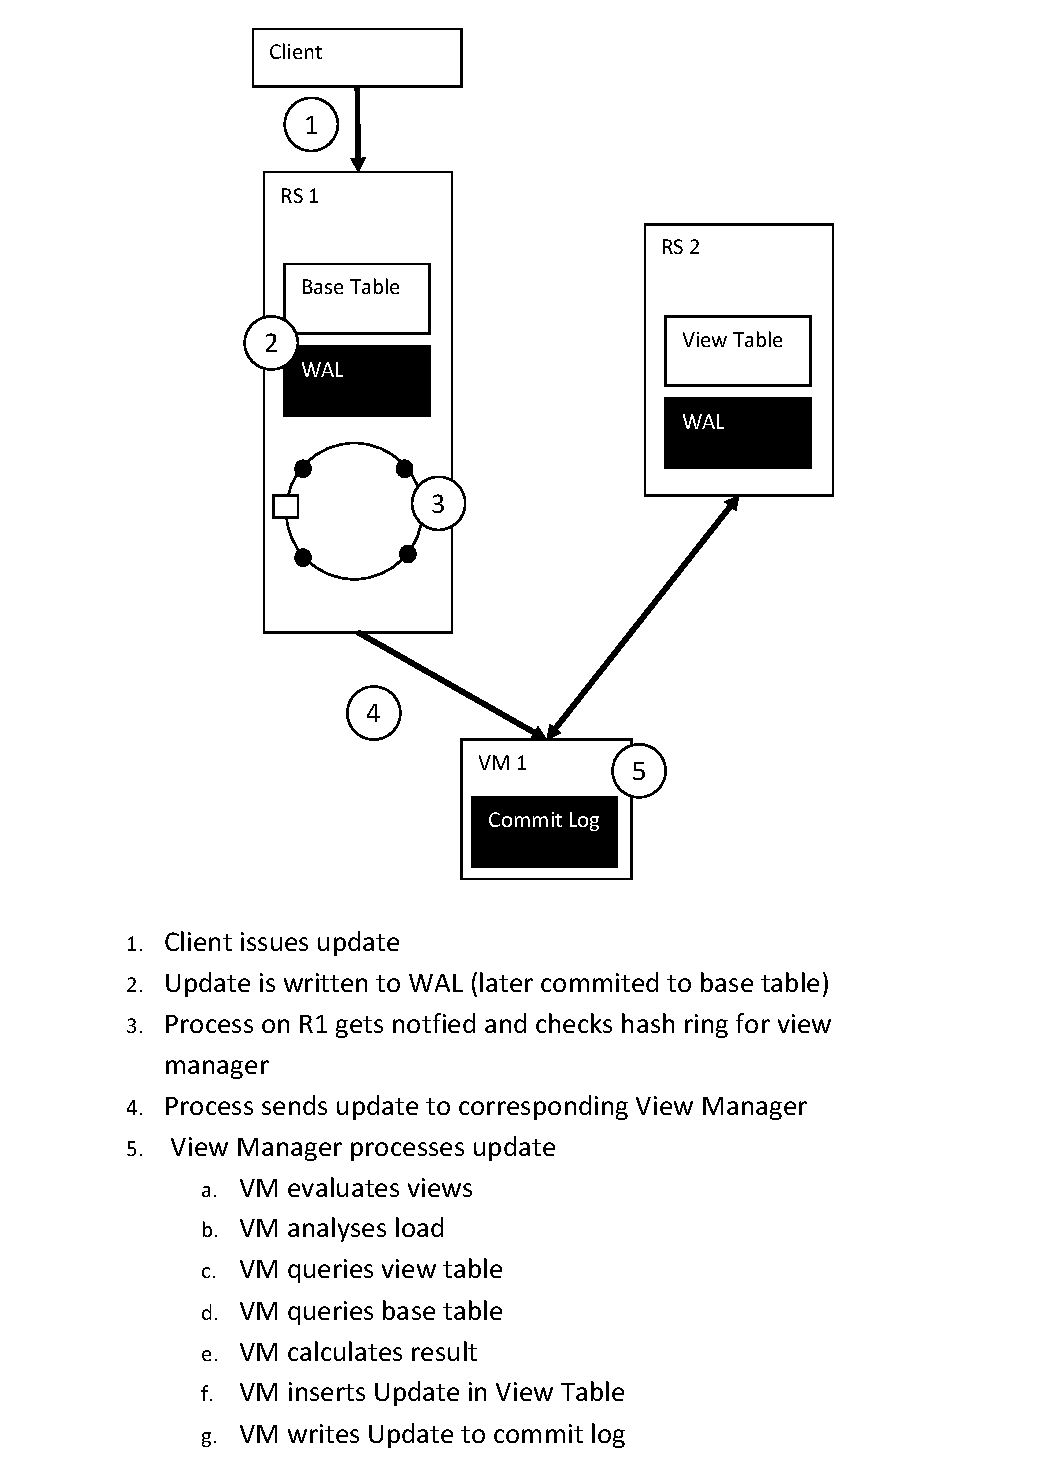
\includegraphics[scale=0.7]{figures/SO_UpdateProcessing}
    \caption{Update Path}
    \label{fig:updatepath}
\end{figure}

\newpage
\section{Status Reports}
\begin{figure}[h!]
  
  \centering
    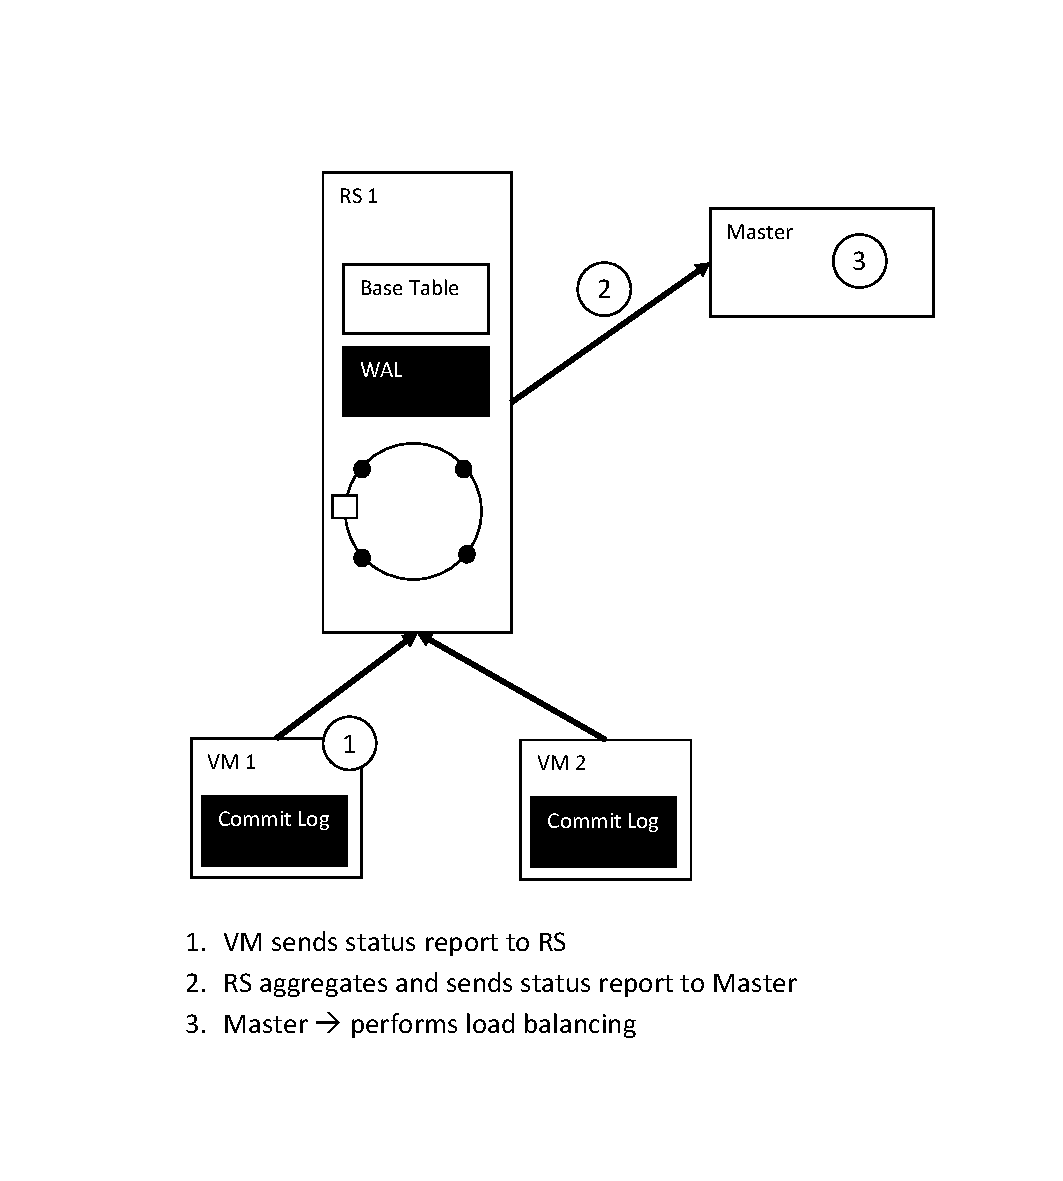
\includegraphics[width=\linewidth]{figures/SO_StatusReports}
    \caption{Status Reports}
    \label{fig:statusreports}
\end{figure}

\chapter{View Consistency}
\label{chapter:viewconsistencyappendix}


\section{Challenges to consistency}
\begin{figure}[h!]
  \centering
    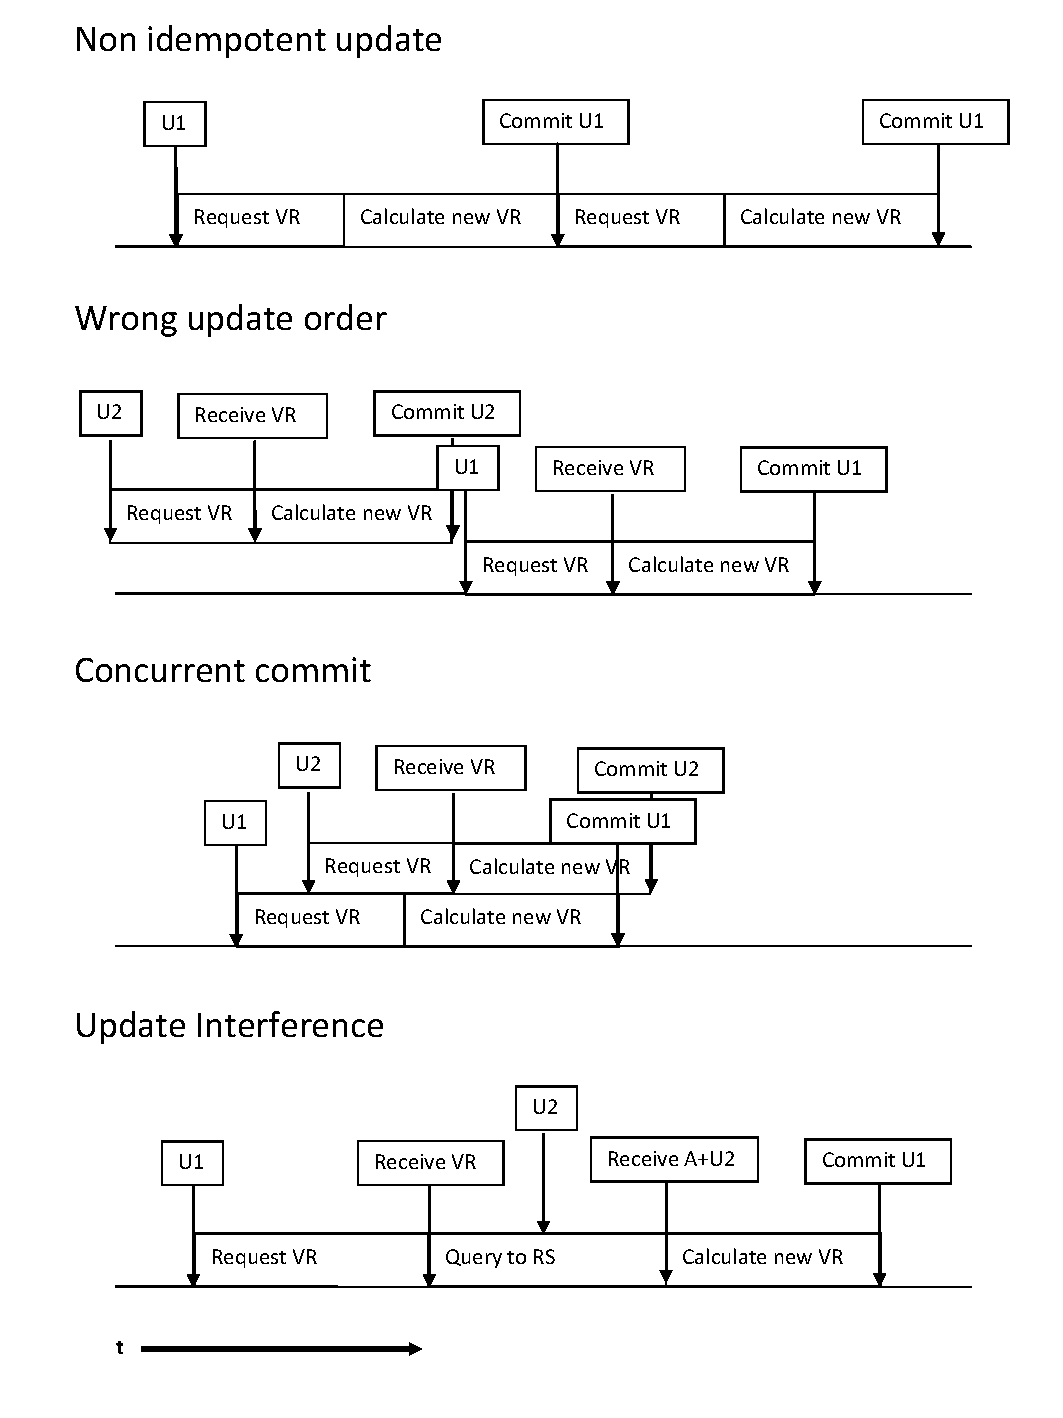
\includegraphics[scale=0.6]{figures/CO_ConsistencyProblems}
     \caption{Consistency threats}
    \label{fig:co_consistencyproblems}
\end{figure}
\newpage

\subsection{Non idempotent view updates}
\begin{figure}[h!]
  \centering
    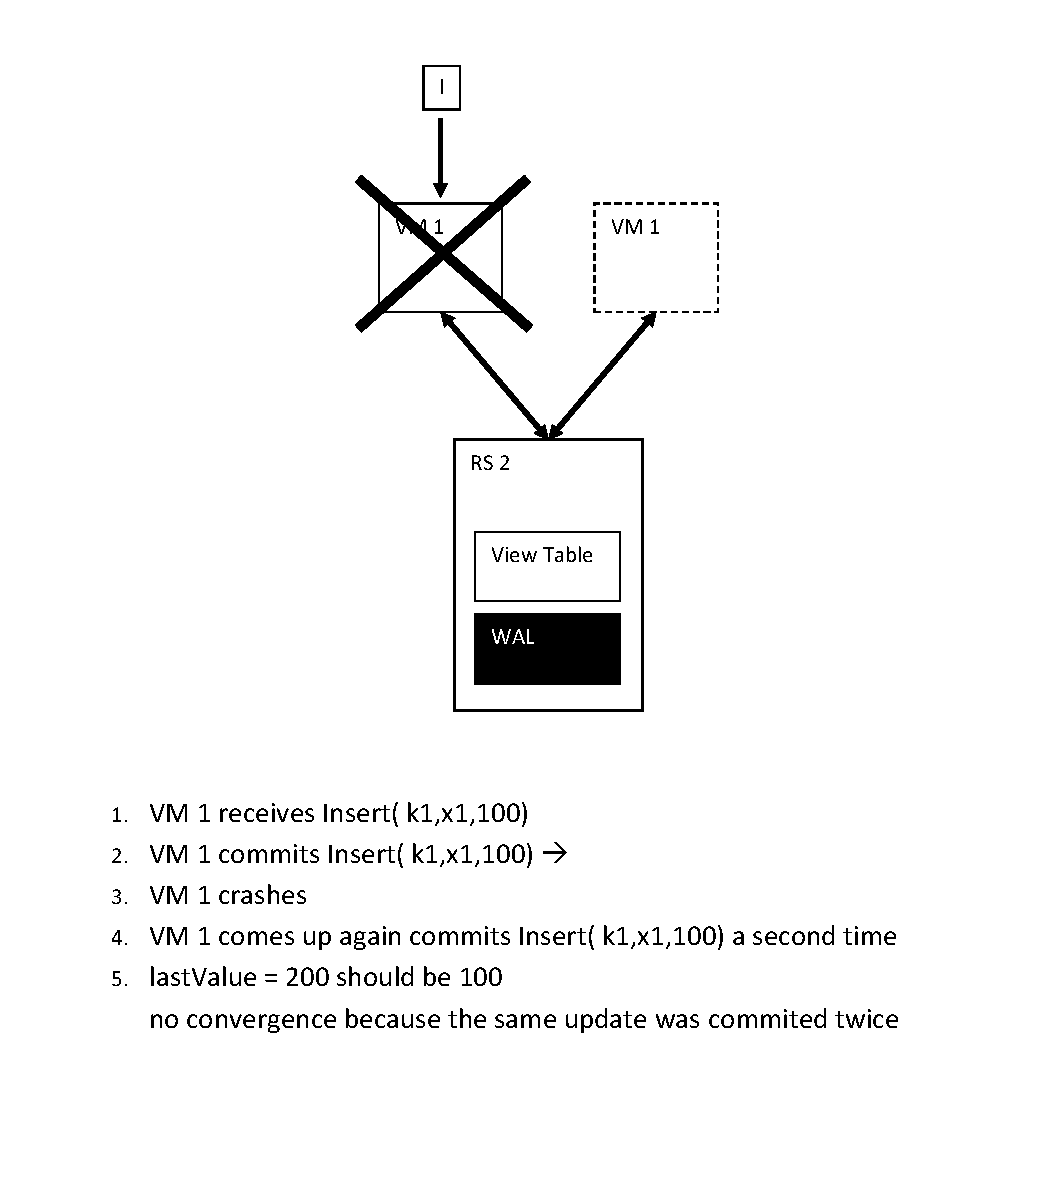
\includegraphics[scale=0.8]{figures/CO_NonIdempotentViewUpdates}
     \caption{Non idempotent view update}
    \label{fig:co_nonidempotentviewupdates}
\end{figure}

\newpage

\subsection{Wrong update order}
\begin{figure}[h!]
  \centering
    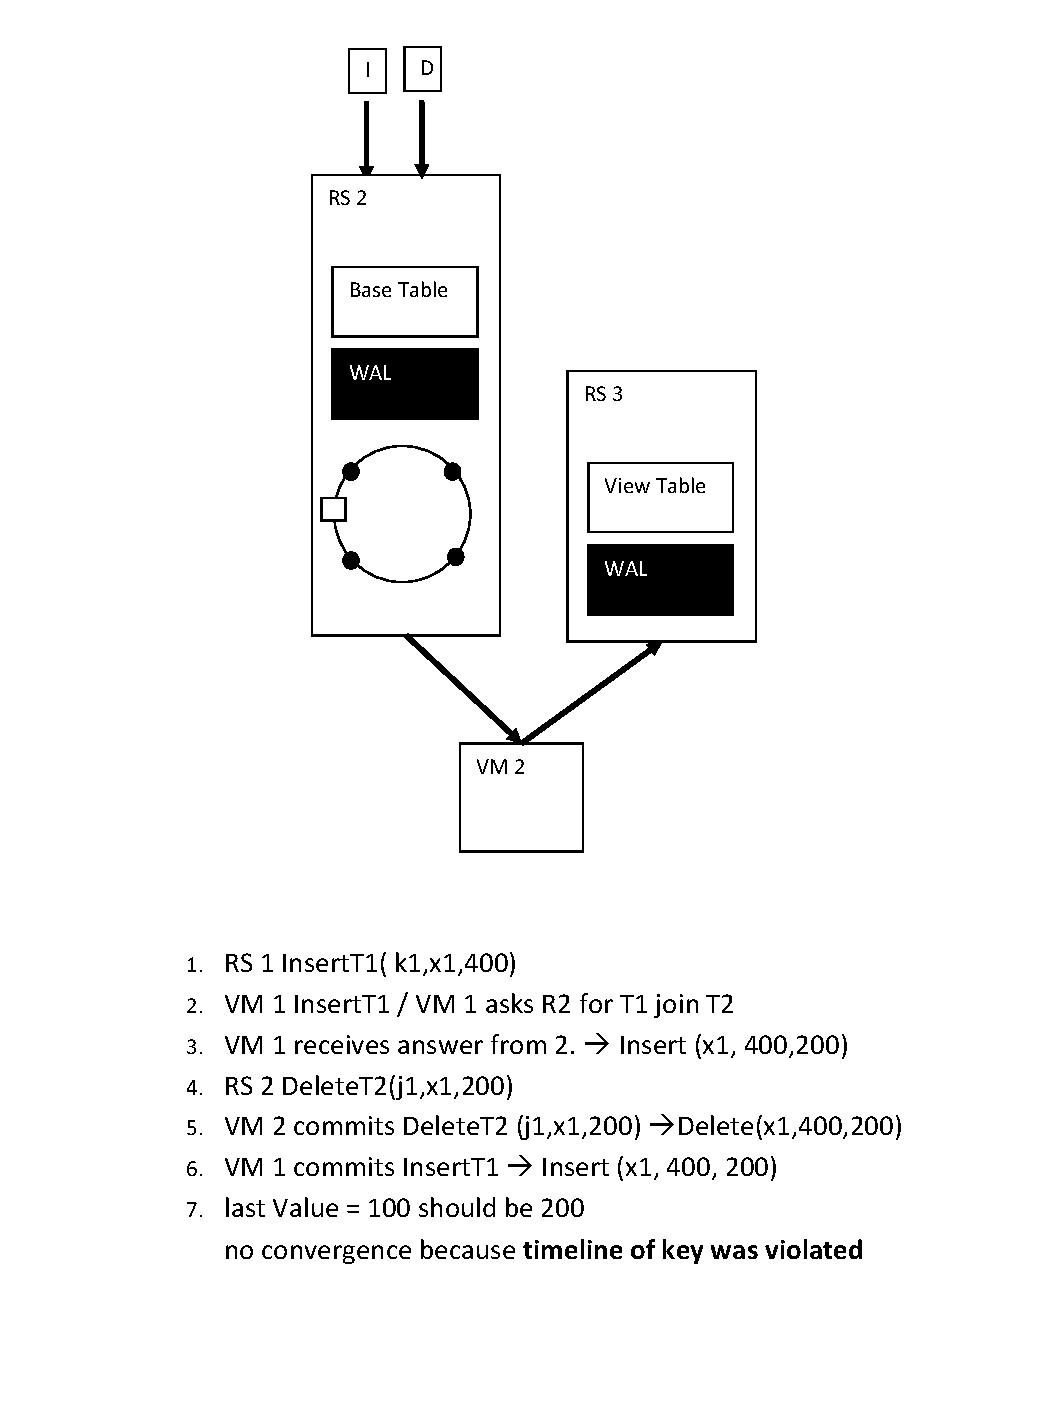
\includegraphics[scale=0.8]{figures/CO_WrongUpdateOrderJoin}
     \caption{Wrong update order join}
    \label{fig:co_wrongupdateorderjoin}
\end{figure}
\newpage
\begin{figure}[h!]
  \centering
    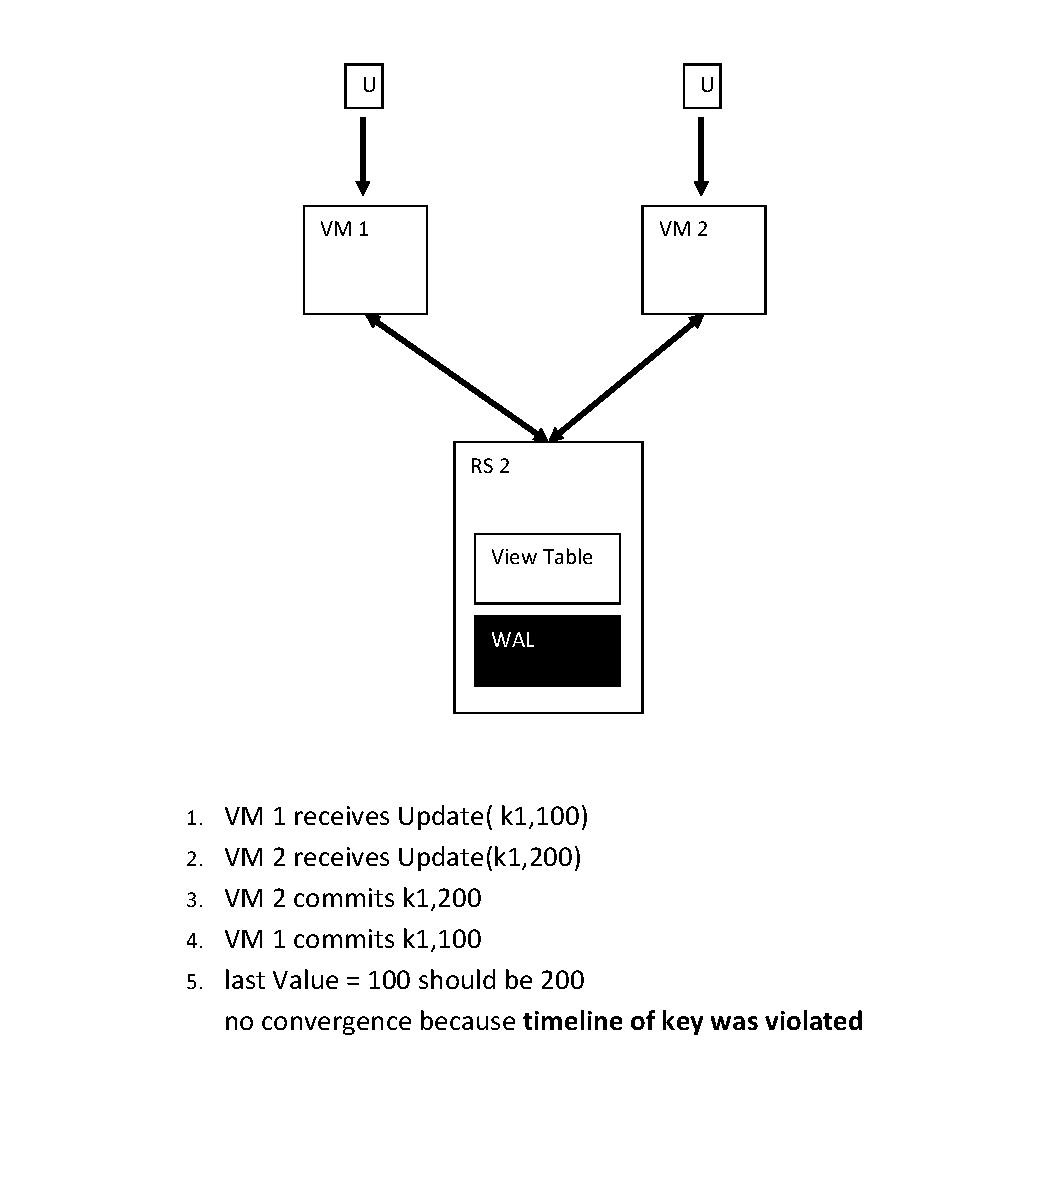
\includegraphics[scale=0.8]{figures/CO_WrongUpdateOrderSelection}
     \caption{Wrong update order Selection}
    \label{fig:co_wrongupdateorderselection}
\end{figure}
\newpage

\subsection{Concurrent commit}
\begin{figure}[h!]
  \centering
    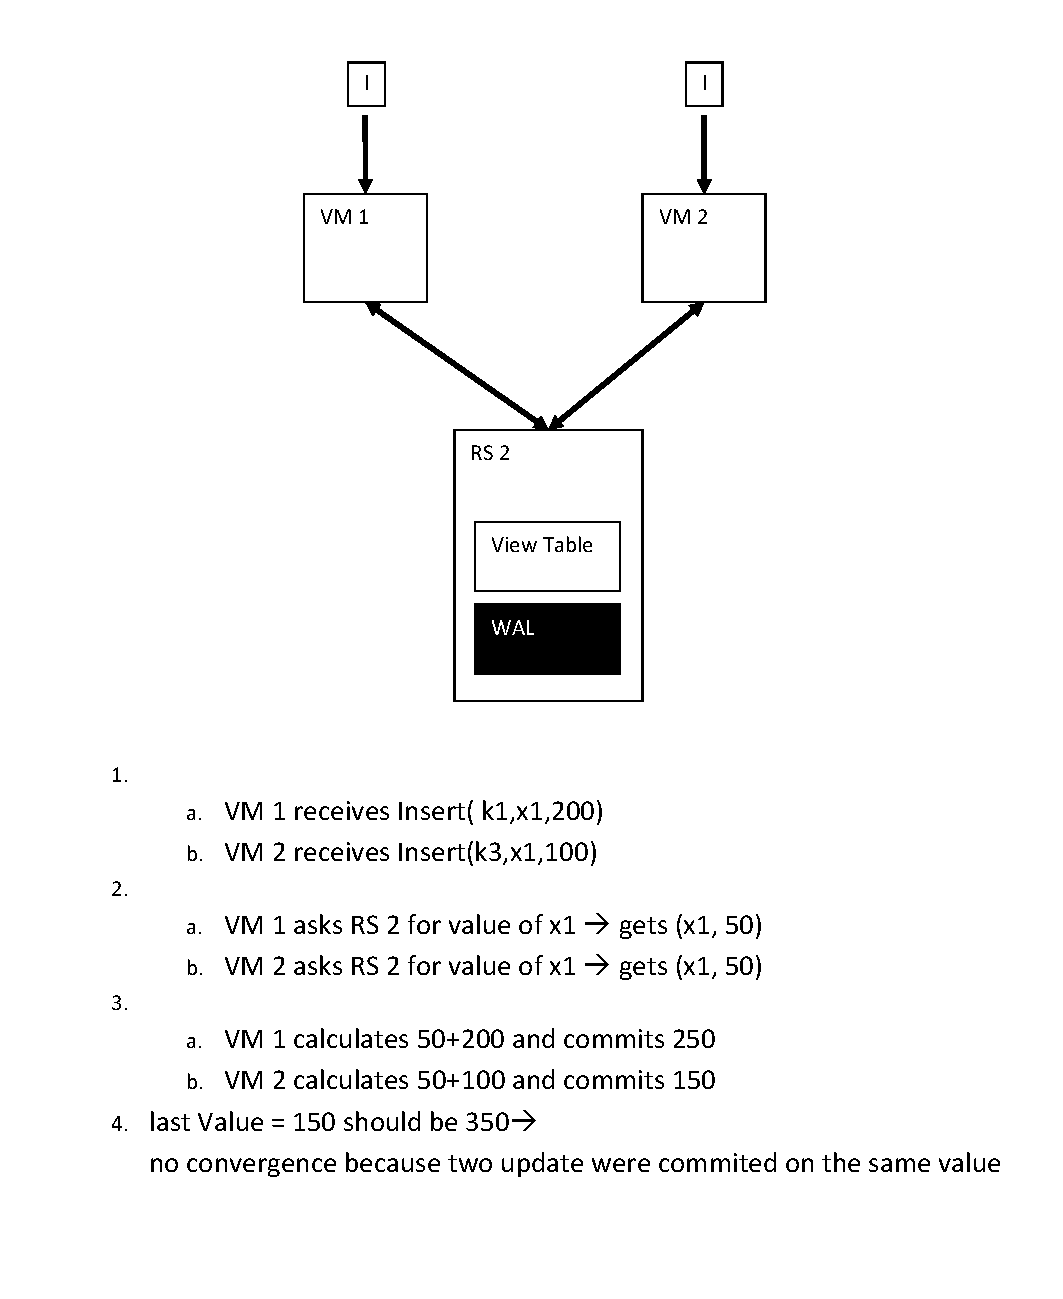
\includegraphics[scale=0.8]{figures/CO_ConcurrentCommitSum}
     \caption{Concurrent commit sum}
    \label{fig:co_concurrentcommitsum}
\end{figure}
\newpage
\begin{figure}[h!]
  \centering
    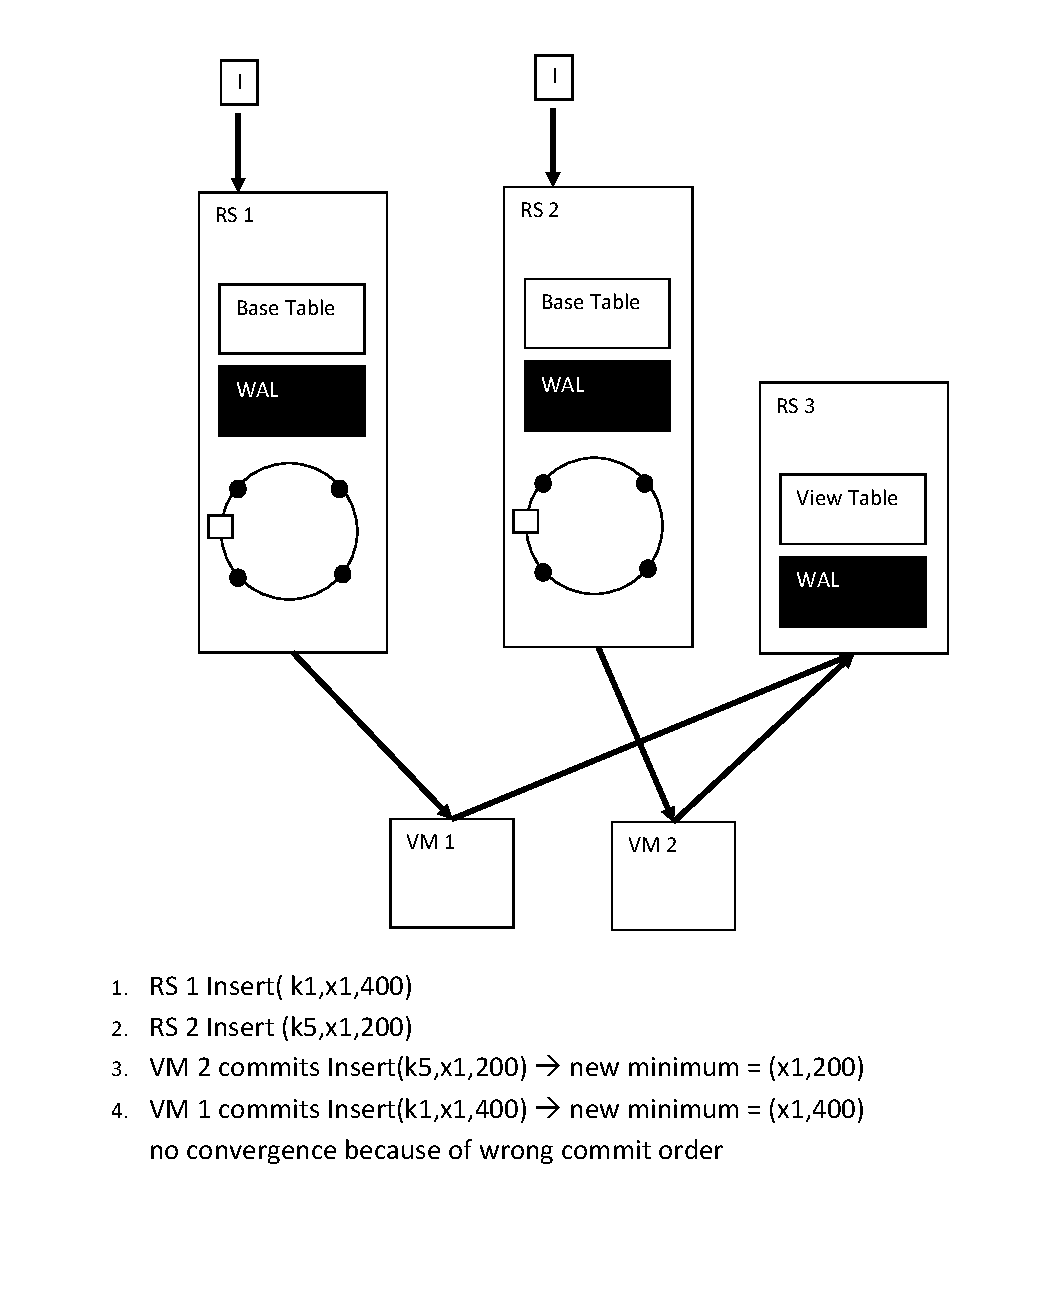
\includegraphics[scale=0.8]{figures/CO_ConcurrentCommitMin}
     \caption{Concurrent commit min}
    \label{fig:co_concurrentcommitmin}
\end{figure}
\newpage

\subsection{Update interference}
\begin{figure}[h!]
  \centering
    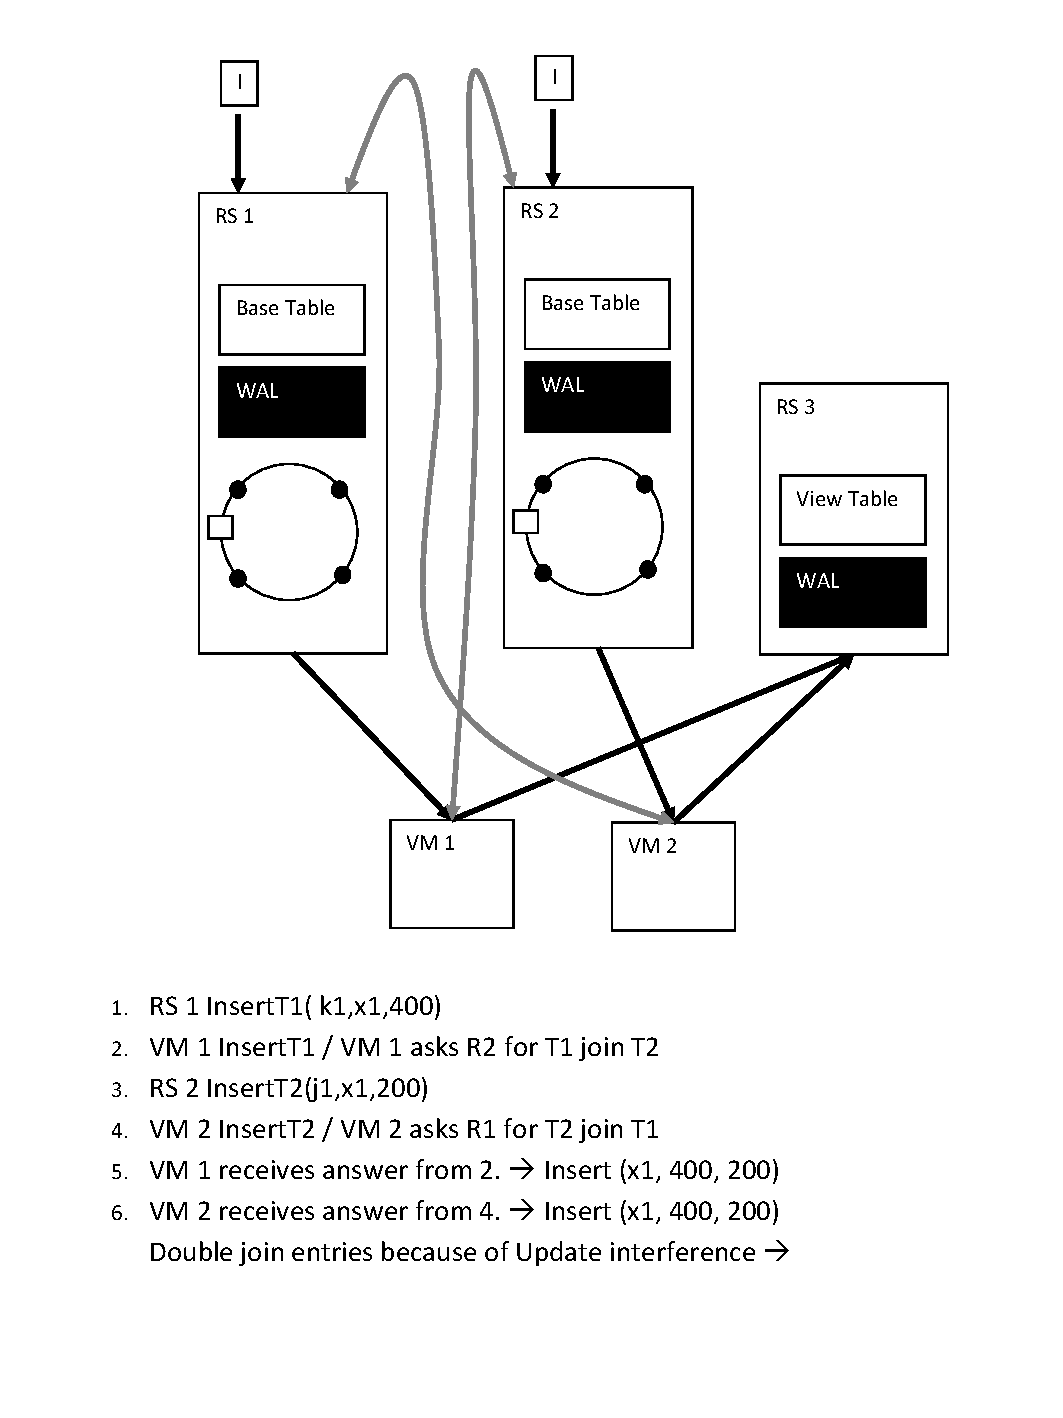
\includegraphics[scale=0.8]{figures/CO_UpdateInterferenceJoin}
     \caption{Update interference join}
    \label{fig:co_updateinterferencejoin}
\end{figure}
\newpage
\begin{figure}[h!]
  \centering
    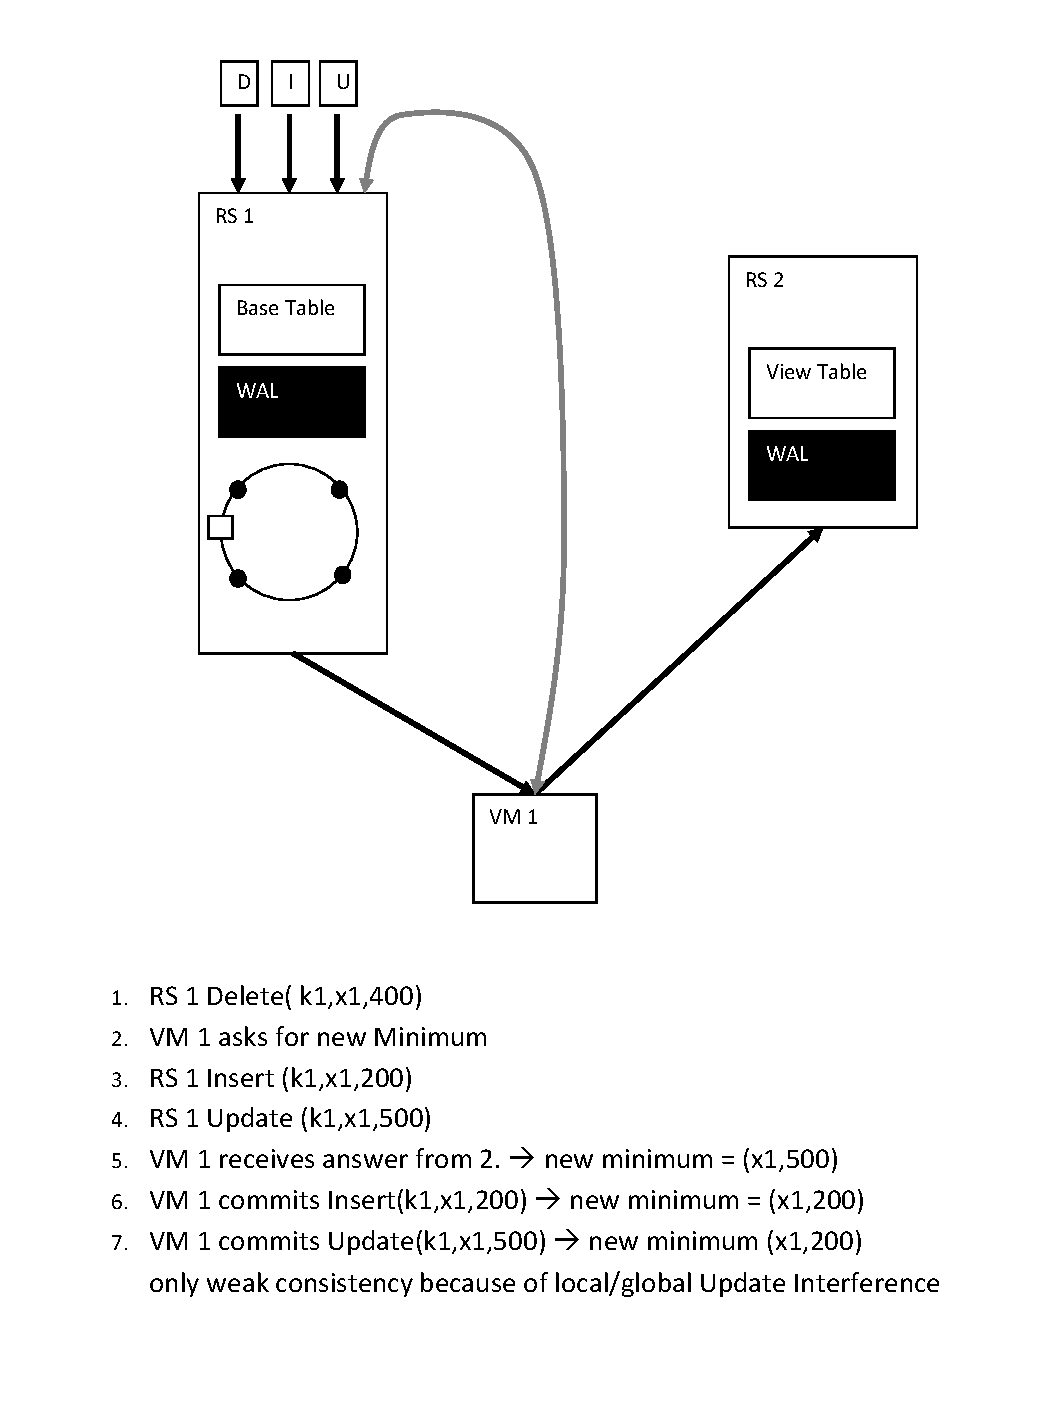
\includegraphics[scale=0.8]{figures/CO_UpdateInterferenceMin}
     \caption{Update interference min}
    \label{fig:co_updateinterferencemin}
\end{figure}
\newpage

\chapter{Load Balancing}
\label{chapter:loadbalancingappendix}


\section{Add View Manager}
\begin{figure}[h!]
  \centering
    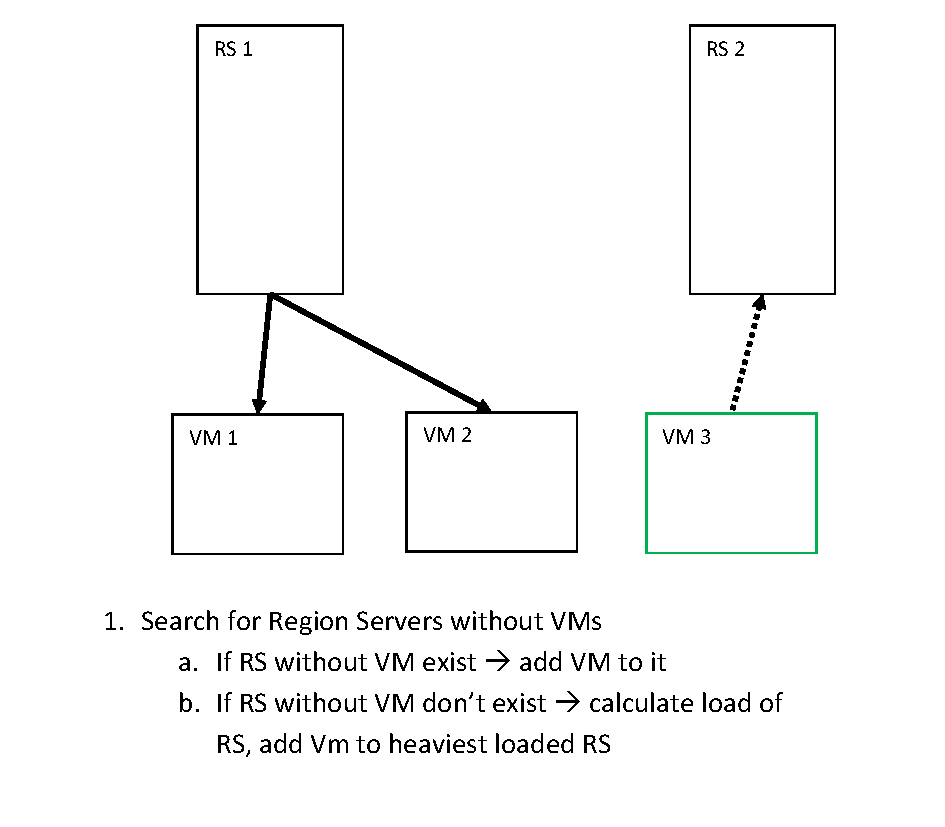
\includegraphics[scale=0.8]{figures/LB_AddViewManager}
     \caption{Add View Manager}
    \label{fig:lb_addviewmanager}
\end{figure}
\newpage

\section{Remove View Manager}
\begin{figure}[h!]
  \centering
    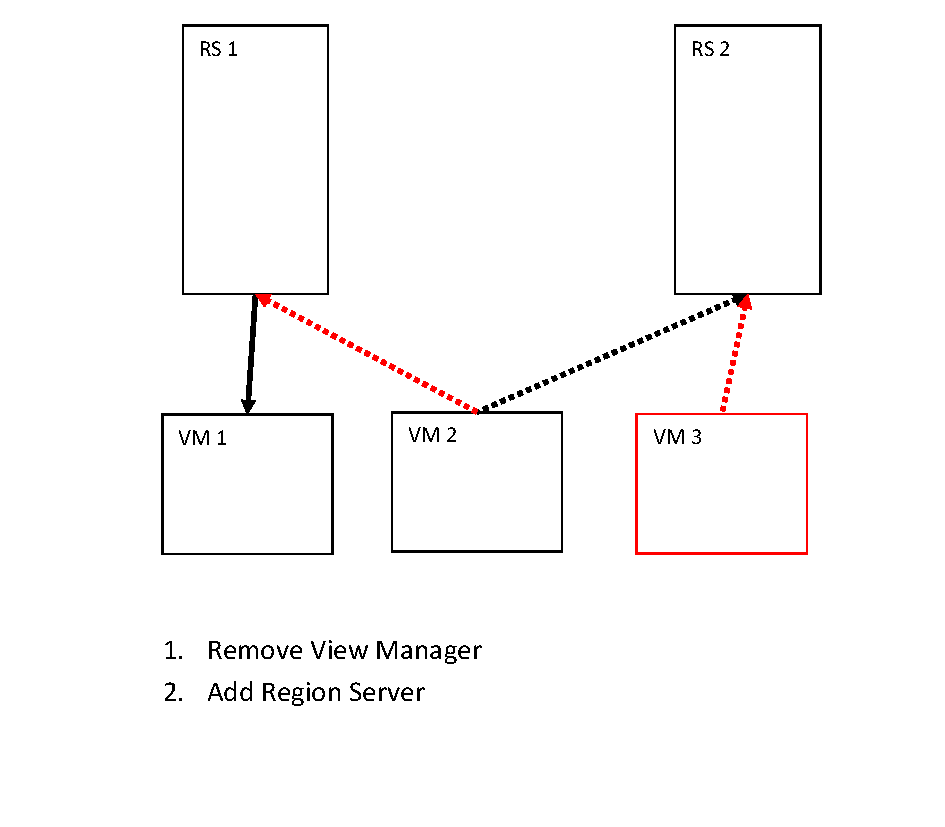
\includegraphics[scale=0.8]{figures/LB_RemoveViewManager}
     \caption{Remove View Manager}
    \label{fig:lb_removeviewmanager}
\end{figure}
\newpage

\section{Add Region Server}
\begin{figure}[h!]
  \centering
    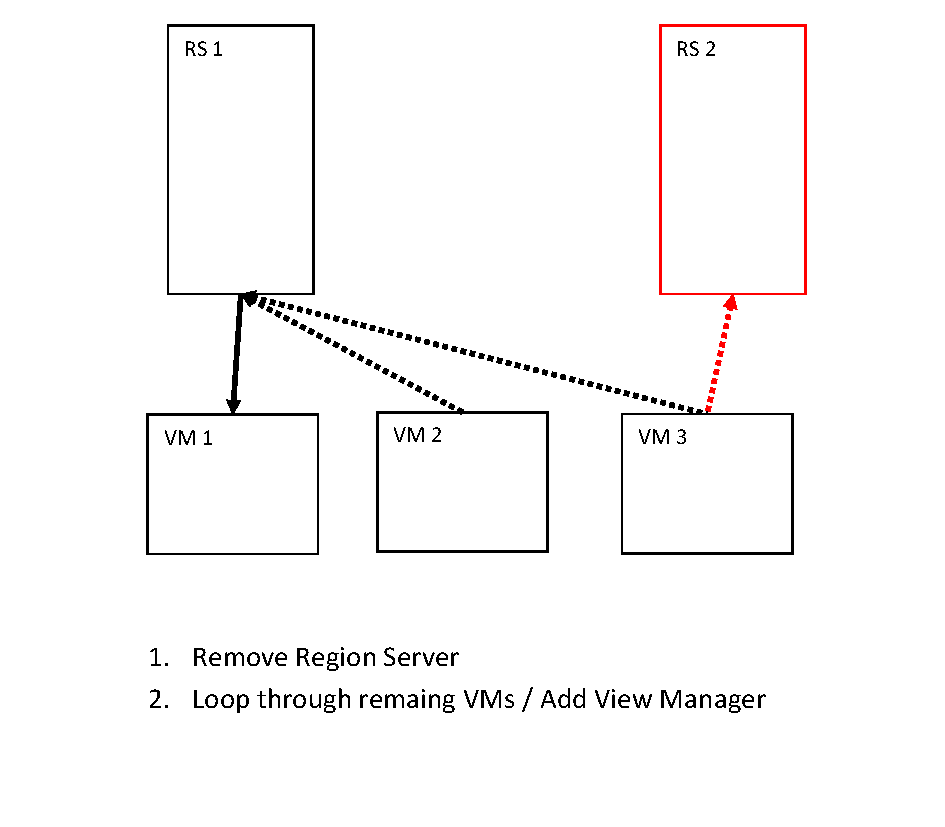
\includegraphics[scale=0.8]{figures/LB_AddRegionServer}
     \caption{Add Region Server}
    \label{fig:lb_addregionserver}
\end{figure}
\newpage

\section{Remove Region Server}
\begin{figure}[h!]
  \centering
    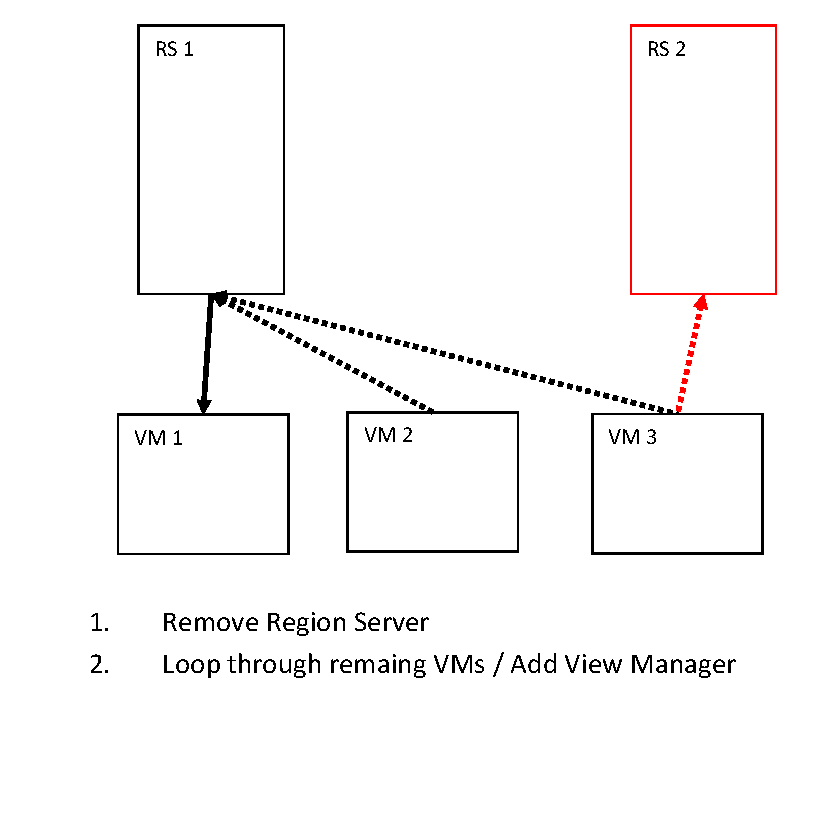
\includegraphics[scale=0.8]{figures/LB_RemoveRegionServer}
    \caption{Remove Region Server}
    \label{fig:lb_removeregionserver}
\end{figure}
\newpage




  \clearemptydoublepage
  
	\bibliography{bibliography/literature}
	
 
\end{document}

